\documentclass[twocolumn]{aastex701}

\usepackage{amsmath}
\usepackage{amssymb}
\usepackage{bm}
\usepackage{booktabs}
\usepackage{array}

\graphicspath{{figures/}}

\newcommand{\SO}{\mathrm{SO}}
\newcommand{\SE}{\mathrm{SE}}
\newcommand{\Nav}{\mathcal{N}}
\newcommand{\R}{\mathbb{R}}
\newcommand{\Exp}{\operatorname{Exp}}
\newcommand{\Log}{\operatorname{Log}}
\newcommand{\wrap}{\operatorname{wrap}_{\pi}}
\newcommand{\diag}{\operatorname{diag}}
\newcommand{\norm}[1]{\left\lVert #1 \right\rVert}

\begin{document}

\title{Adaptive Error-State Kalman Filtering for Indoor Robot Localization Using Synthetic LiDAR and Beacon Measurements}

\author{Arun Showry Busani.}
\affiliation{Georgia Institute of Technology}
\email{abusani3@gatech.edu}

\begin{abstract}
This work is on a filtering pipeline for two-dimensional indoor localization with synthetic LiDAR pose measurements and fixed radio beacons. The estimator is an error-state extended Kalman filter whose nominal state is a five-degree-of-freedom 2D NavState matrix containing heading, position, and velocity. Prediction uses noisy body-frame acceleration and yaw rate, while measurement updates use beacon ranges with either fixed or range/RSSI-adaptive covariance and synthetic LiDAR pose measurements with scan-quality-dependent covariance. Three generated indoor scenarios are evaluated: an open hallway with side rooms, a multi-room map, and a larger dense map. Across the results, dead reckoning gives a mean position RMSE of 7.398 m, fixed-covariance beacon fusion gives 0.326 m, adaptive beacon fusion gives 0.286 m, LiDAR-only fusion gives 0.0968 m, and LiDAR plus adaptive beacons gives 0.0891 m. This shows that the adaptive beacon model improves aggregate beacon-only localization relative to fixed covariance, while the synthetic LiDAR pose update is the dominant correction source in the tested scenarios.

\end{abstract}

\keywords{Localization, Kalman filtering, LiDAR, radio beacons, manifold methods, sensor fusion}

\section{Introduction}

Indoor mobile robots often operate in environments where individual sensing modalities are intermittently informative. Range-bearing or scan-based perception can be degraded by weak geometric structure, while radio or beacon measurements can be affected by range limits, wall attenuation, and changing visibility. The repository studied here isolates this sensor-fusion problem in a reproducible synthetic setting: a ground robot moves through known 2D wall-segment maps, receives noisy odometry-like prediction inputs, and fuses intermittent LiDAR-derived pose measurements with range-only beacon measurements.

The implemented problem is localization rather than SLAM. The map and beacon locations are known, and the estimator does not estimate wall geometry or beacon positions. The main question is whether a beacon range covariance adapted from robot-side measurements, specifically measured range and RSSI, improves an error-state Kalman filter relative to a fixed beacon covariance. A separate LiDAR-only and LiDAR-plus-beacon comparison quantifies the role of scan-derived pose corrections.

The state representation follows the manifold-aware structure used in modern robotics estimation libraries such as GTSAM \citep{dellaert2022gtsam,gtsamConcepts,dellaert2012gtsam,dellaertKaess2017factor}. Although the code does not call GTSAM, it uses the same conceptual separation between a nominal state on a nonlinear space and a local vector perturbation used for linearization. This is relevant because robot orientation belongs to a rotation group, and applying heading corrections by unconstrained vector addition can obscure the distinction between global state variables and local tangent coordinates. The filter therefore stores the nominal estimate as a matrix NavState and applies prediction and correction increments through a NavState exponential map.

\section{System Overview}

The repository is organized as a reproducible MATLAB pipeline. The top-level script \texttt{main.m} loads configuration, resets generated outputs, generates synthetic datasets, runs all filter configurations, and exports tables and figures. The modular scripts \texttt{generate\_dataset.m}, \texttt{run\_filters.m}, and \texttt{generate\_outputs.m} separate dataset creation, filtering, and post-processing.

\subsection{Pipeline}

For each configured scenario, \path{generate_scenario_dataset.m} creates a wall-segment map, beacon definitions, a wall-validating ground-truth trajectory, noisy prediction inputs, beacon measurements, LiDAR scans, and synthetic LiDAR pose measurements. The data is then loaded by \texttt{run\_filter\_case.m}, which evaluates five cases using the same truth and measurement files. Finally, \texttt{collect\_results\_tables.m} computes RMSE and sensor availability metrics, and \texttt{generate\_project\_figures.m} exports the result figures used in this manuscript.

\subsection{Ground Robot State}

The ground robot state is a 2D NavState matrix with heading, position, and velocity. The stored truth arrays use \texttt{truth.p} and \texttt{truth.v} as \(2 \times N\) matrices, \texttt{truth.theta} as a length-\(N\) heading sequence, and \texttt{truth.X} as \(4 \times 4 \times N\) NavState matrices. No accelerometer bias, gyroscope bias, clock state, or beacon state is estimated by the EKF.

\subsection{Environment Representation}

The environment is a known 2D floor plan represented by line-segment walls. Each wall stores endpoints, thickness, material factor, and a text label. Openings are represented by gaps between wall segments. The simulator uses wall geometry for trajectory validation, beacon attenuation, and LiDAR ray casting. The filter does not receive wall-crossing counts or hidden attenuation values.

\subsection{Beacon and LiDAR Simulation}

Beacon simulation is implemented in \texttt{simulate\_beacon\_measurements.m}. Each beacon is fixed in the map and has a range limit, penetration budget, RSSI reference, RSSI threshold, and range-noise parameters. The simulator rejects measurements when range, attenuation, RSSI, or random dropout tests fail. The filter receives only timestamp, beacon ID, measured range, RSSI, and availability.

LiDAR simulation is implemented in \texttt{simulate\_lidar\_measurements.m}. The scan model ray-casts 181 beams across a \(270^\circ\) field of view with a 12 m maximum range. The EKF does not update on raw beams. Instead, the simulator produces a synthetic pose measurement and covariance whose standard deviations depend on scan quality. 

\subsection{Estimation Backend}

The estimation backend is an error-state EKF. Prediction is driven by noisy body-frame acceleration and yaw-rate measurements. Corrections are applied using scalar beacon range residuals and three-dimensional LiDAR pose residuals. The covariance is maintained in the local tangent ordering
\begin{equation}
    \delta x =
    \begin{bmatrix}
    \delta \theta & \delta p_x & \delta p_y & \delta v_x & \delta v_y
    \end{bmatrix}^{T}.
\end{equation}
After each correction, \texttt{ekf\_tangent\_update.m} maps the translational parts of the correction into the local group frame and composes the result onto the nominal NavState using \texttt{navstate\_exp.m}.

\section{Methodology}

\subsection{State Definition}

The implemented nominal state is the 2D NavState matrix
\begin{equation}
X =
\begin{bmatrix}
R(\theta) & p & v \\
0_{1\times 2} & 1 & 0 \\
0_{1\times 2} & 0 & 1
\end{bmatrix},
\label{eq:navstate}
\end{equation}
where \(R(\theta)\in \SO(2)\), \(p=[x\ y]^T\in\R^2\), and \(v=[\dot{x}\ \dot{y}]^T\in\R^2\). This state has five degrees of freedom:
\begin{equation}
    x_{\mathrm{dof}} =
    \begin{bmatrix}
    \theta & x & y & \dot{x} & \dot{y}
    \end{bmatrix}^{T}.
\end{equation}
The covariance \(P\in\R^{5\times 5}\) is not stored over the matrix entries of \(X\). It is stored over local tangent coordinates ordered as
\begin{equation}
    \delta x =
    \begin{bmatrix}
    \delta \theta &
    \delta p_x &
    \delta p_y &
    \delta v_x &
    \delta v_y
    \end{bmatrix}^{T}.
\label{eq:error_state}
\end{equation}

The helper \texttt{make\_navstate.m} constructs Eq.~(\ref{eq:navstate}); \texttt{navstate\_components.m} extracts \(\theta\), \(p\), and \(v\). The implementation uses a 2D analog of the GTSAM NavState idea, where pose and velocity are treated as one navigation state on a smooth group-like space \citep{gtsamNavigation,gtsamNavState,forster2015imu}.

\subsection{NavState Exponential Map}

Prediction and correction increments are mapped back to the nominal state by \texttt{navstate\_exp.m}. For a local increment
\begin{equation}
    \delta =
    \begin{bmatrix}
    \phi & \rho_x & \rho_y & \nu_x & \nu_y
    \end{bmatrix}^{T},
\end{equation}
define \(\rho=[\rho_x\ \rho_y]^T\), \(\nu=[\nu_x\ \nu_y]^T\), and
\begin{equation}
    A(\phi)=1-\frac{\phi^2}{6}, \qquad
    B(\phi)=\frac{\phi}{2}-\frac{\phi^3}{24}.
\end{equation}
The code uses the third-order Taylor left-Jacobian approximation
\begin{equation}
    J(\phi)=
    \begin{bmatrix}
    A(\phi) & -B(\phi) \\
    B(\phi) & A(\phi)
    \end{bmatrix}.
\end{equation}
The returned increment is
\begin{equation}
\Exp(\delta)=
\begin{bmatrix}
R(\phi) & J(\phi)\rho & J(\phi)\nu \\
0_{1\times 2} & 1 & 0 \\
0_{1\times 2} & 0 & 1
\end{bmatrix}.
\label{eq:nav_exp}
\end{equation}
The nominal update is group composition:
\begin{equation}
    X^{+}=X\,\Exp(\delta).
\end{equation}
Consequently, heading is updated on \(\SO(2)\), and position and velocity increments are rotated by the current nominal frame through matrix multiplication.

\subsection{Prediction Model}

The prediction input generated by \path{simulate_prediction_inputs.m} is body-frame acceleration and yaw rate:
\begin{equation}
    u_k =
    \begin{bmatrix}
    a_{b,k}^{T} & \omega_k
    \end{bmatrix}^{T}.
\end{equation}
The simulator computes true body-frame acceleration from the saved truth trajectory, then adds a scenario-constant bias and white noise. The filter does not estimate these biases. The configured generation noise is \(\sigma_a=0.08~\mathrm{m/s^2}\) and \(\sigma_\omega=0.012~\mathrm{rad/s}\), with per-scenario bias standard deviations \(0.018~\mathrm{m/s^2}\) and \(0.004~\mathrm{rad/s}\). The filter prediction covariance uses the larger values \(\sigma_a=0.11~\mathrm{m/s^2}\) and \(\sigma_\omega=0.018~\mathrm{rad/s}\).

At timestep \(k\), \texttt{propagate\_navstate.m} extracts \((\theta_k,p_k,v_k)\), forms \(R_k=R(\theta_k)\), and computes
\begin{align}
    \phi_k &= \omega_k \Delta t,\\
    \rho_k &= R_k^T(v_k\Delta t)+\frac{1}{2}a_{b,k}\Delta t^2,\\
    \nu_k &= a_{b,k}\Delta t.
\end{align}
The nominal propagation is
\begin{equation}
    X_{k+1|k}=X_{k|k}\Exp
    \left(
    \begin{bmatrix}
    \phi_k & \rho_k^T & \nu_k^T
    \end{bmatrix}^{T}
    \right).
\label{eq:prediction}
\end{equation}
For small \(\phi_k\), Eq.~(\ref{eq:prediction}) reduces to the familiar planar kinematic update \(p_{k+1}\approx p_k+v_k\Delta t+\frac{1}{2}R_k a_{b,k}\Delta t^2\), \(v_{k+1}\approx v_k+R_k a_{b,k}\Delta t\), and \(\theta_{k+1}\approx \theta_k+\omega_k\Delta t\).

The covariance propagation follows the EKF form \citep{simon2006optimal,brownHwang2012random}
\begin{equation}
    P_{k+1|k}=F_k P_{k|k}F_k^T+G_k Q_u G_k^T+Q_{\mathrm{floor}},
\label{eq:cov_prediction}
\end{equation}
where
\begin{equation}
    Q_u=\diag(\sigma_a^2,\sigma_a^2,\sigma_\omega^2)
\end{equation}
and
\begin{equation}
    Q_{\mathrm{floor}}=\diag(10^{-7},10^{-6},10^{-6},10^{-5},10^{-5}).
\end{equation}
Let
\begin{equation}
    S_2=
    \begin{bmatrix}
    0 & -1\\
    1 & 0
    \end{bmatrix},
    \qquad
    c_k=R_k S_2 a_{b,k}.
\end{equation}
The implemented linearization is
\begin{equation}
F_k =
\begin{bmatrix}
1 & 0_{1\times 2} & 0_{1\times 2}\\
\frac{1}{2}c_k\Delta t^2 & I_2 & \Delta t I_2\\
c_k\Delta t & 0_{2\times 2} & I_2
\end{bmatrix},
\label{eq:F}
\end{equation}
with block rows ordered as \(\theta,p,v\), and
\begin{equation}
G_k =
\begin{bmatrix}
0_{1\times 2} & \Delta t\\
\frac{1}{2}R_k\Delta t^2 & 0_{2\times 1}\\
R_k\Delta t & 0_{2\times 1}
\end{bmatrix}.
\label{eq:G}
\end{equation}

\subsection{Beacon Simulation Model}

For beacon \(i\), the true range and simulator-side hidden attenuation are
\begin{align}
    d_{i,k} &= \norm{p_k-b_i},\\
    A_{i,k} &= \sum_{j\in\mathcal{I}_{i,k}} t_j m_j,
\end{align}
where \(b_i\) is the known beacon position, \(\mathcal{I}_{i,k}\) is the set of wall segments intersected by the robot-to-beacon line segment, \(t_j\) is wall thickness, and \(m_j\) is material factor. This attenuation is computed by \texttt{wall\_attenuation.m} and is privileged simulator knowledge.

The simulator rejects a beacon measurement if any of the following conditions holds:
\begin{align}
    d_{i,k} &> d_{\max,i},&
    A_{i,k} &> A_{\max,i},&
    \mathrm{RSSI}_{i,k} &< \mathrm{RSSI}_{\min},
\end{align}
or if a random dropout draw succeeds. Before the RSSI threshold test, the implemented signal model is
\begin{equation}
    \mathrm{RSSI}_{i,k}
    =
    r_{0,i}
    -\alpha_d d_{i,k}
    -\alpha_w A_{i,k}
    + n_{s,k},
\label{eq:rssi}
\end{equation}
where \(\alpha_d=3.0\), \(\alpha_w=34.0\), \(n_{s,k}\sim\mathcal{N}(0,\sigma_s^2)\), and \(\sigma_s=2.2\). The repository stores a \texttt{path\_loss\_exponent} field for each beacon, but the implemented RSSI model is the linear distance-and-wall model in Eq.~(\ref{eq:rssi}), not a logarithmic path-loss model. The model is therefore a controlled synthetic degradation model rather than a full radio propagation model \citep{rappaport2002wireless}.

If the measurement remains available, the simulator uses
\begin{equation}
    \sigma_{r,i,k}
    =
    \sigma_{0}
    + k_d d_{i,k}
    + k_s\max(0,r_{0,i}-\mathrm{RSSI}_{i,k})
\end{equation}
with \(\sigma_0=0.12~\mathrm{m}\), \(k_d=0.025\), and \(k_s=0.006\). The measured range is
\begin{equation}
    z_{i,k}=d_{i,k}+n_{r,k},\qquad
    n_{r,k}\sim\mathcal{N}(0,\sigma_{r,i,k}^{2}).
\end{equation}

\subsection{Beacon EKF Update}

The filter-side beacon measurement function is
\begin{equation}
    h_i(X)=\norm{p-b_i}.
\end{equation}
The implementation clamps the predicted range used in the residual and Jacobian to the configured minimum \(d_{\min}=0.20~\mathrm{m}\):
\begin{equation}
    \hat{d}_{i,k}=\max\left(\norm{\hat{p}_k-b_i},d_{\min}\right).
\end{equation}
The scalar residual is
\begin{equation}
    r_{i,k}=z_{i,k}-\hat{d}_{i,k}.
\end{equation}
For the tangent ordering in Eq.~(\ref{eq:error_state}), the implemented beacon Jacobian is
\begin{equation}
H_{i,k}=
\begin{bmatrix}
0 &
\dfrac{\hat{p}_{x,k}-b_{x,i}}{\hat{d}_{i,k}} &
\dfrac{\hat{p}_{y,k}-b_{y,i}}{\hat{d}_{i,k}} &
0 & 0
\end{bmatrix}.
\label{eq:beacon_H}
\end{equation}

The fixed-covariance beacon case uses
\begin{equation}
    R_{i,k}=0.55^2.
\end{equation}
The adaptive beacon case uses only robot-side values, measured range and RSSI:
\begin{equation}
    \hat{\sigma}_{i,k}
    =
    \sigma_0
    + k_d\max(z_{i,k},0)
    + k_s\max(0,r_{0,i}-\mathrm{RSSI}_{i,k}),
\label{eq:adaptive_sigma}
\end{equation}
followed by the lower bound \(\hat{\sigma}_{i,k}\geq 0.05~\mathrm{m}\), and \(R_{i,k}=\hat{\sigma}_{i,k}^2\). The filter does not use true attenuation, true range before noise, wall counts, or wall thickness values during the beacon update.

\subsection{LiDAR Simulation and Pose Update}

For each scan, \texttt{raycast\_map.m} casts beams at angles
\begin{equation}
    \alpha_{\ell,k}=\theta_k+\beta_{\ell},
\end{equation}
where \(\beta_{\ell}\) spans the configured \(270^\circ\) field of view. The range for beam \(\ell\) is the closest wall intersection distance within 12 m, or the maximum range if no intersection exists. Valid returns are corrupted by independent Gaussian range noise with \(\sigma=0.035~\mathrm{m}\); invalid returns are stored at max range.

The scan quality score is computed from valid return fraction \(f_v\), capped normalized range spread \(s_r\), and near-wall fraction \(f_n\):
\begin{align}
    q_k=\operatorname{clamp}\big(
    &0.10+0.50f_v+0.25s_r+0.15f_n,\nonumber\\
    &0.05,\ 0.98
    \big).
\end{align}
For the open-hallway scenario, the code subtracts 0.18 from this score when the range spread is less than 0.16, modeling reduced geometric diversity in hallway-like scans.

At the LiDAR pose-update rate, the simulator forms
\begin{equation}
    z_{\ell,k} =
    \begin{bmatrix}
    x_k & y_k & \theta_k
    \end{bmatrix}^{T}
    + n_{\ell,k},
\end{equation}
when the quality and valid-return tests pass and no random dropout occurs. The covariance is
\begin{equation}
R_{\ell,k}=\diag
\left(
\sigma_{xy,k}^{2},\sigma_{xy,k}^{2},\sigma_{\theta,k}^{2}
\right),
\end{equation}
with
\begin{align}
    \sigma_{xy,k} &= 0.08+0.55(1-q_k)^2,\\
    \sigma_{\theta,k} &= 1.2^\circ+7.0^\circ(1-q_k)^2.
\end{align}
The EKF measurement model is
\begin{equation}
    h_{\ell}(X)=
    \begin{bmatrix}
    p_x & p_y & \theta
    \end{bmatrix}^{T},
\end{equation}
with residual
\begin{equation}
    r_{\ell,k}=
    \begin{bmatrix}
    z_x-\hat{p}_x\\
    z_y-\hat{p}_y\\
    \wrap(z_\theta-\hat{\theta})
    \end{bmatrix}
\end{equation}
and Jacobian
\begin{equation}
H_{\ell}=
\begin{bmatrix}
0 & 1 & 0 & 0 & 0\\
0 & 0 & 1 & 0 & 0\\
1 & 0 & 0 & 0 & 0
\end{bmatrix}.
\label{eq:lidar_H}
\end{equation}
This synthetic pose-measurement interface is a deliberate simplification consistent with probabilistic range-sensor modeling practice \citep{thrun2005probabilistic,dellaertHutchinson2023robotics}; no scan matching is implemented.

\subsection{EKF Correction}

Both beacon and LiDAR updates call \texttt{ekf\_tangent\_update.m}. For residual \(r_k\), Jacobian \(H_k\), and measurement covariance \(R_k\), the innovation covariance and Kalman gain are
\begin{align}
    S_k &= H_kP_{k|k-1}H_k^T+R_k,\\
    K_k &= P_{k|k-1}H_k^T S_k^{-1}.
\end{align}
The tangent correction is
\begin{equation}
    \delta x_k=K_k r_k.
\end{equation}
If \(\norm{\delta x_k}>4.0\), the code scales the correction to norm 4.0 before applying it. Let \(\delta p_k\) and \(\delta v_k\) denote the world-frame translational components of \(\delta x_k\). Before composition, the code converts those components into the local nominal frame:
\begin{equation}
    \delta_{\mathrm{group},k}=
    \begin{bmatrix}
    \delta \theta_k\\
    \hat{R}_k^T\delta p_k\\
    \hat{R}_k^T\delta v_k
    \end{bmatrix}.
\end{equation}
The nominal state update is
\begin{equation}
    X_{k|k}=X_{k|k-1}\Exp(\delta_{\mathrm{group},k}).
\end{equation}
The covariance uses the Joseph form
\begin{equation}
P_{k|k}
=
(I-K_kH_k)P_{k|k-1}(I-K_kH_k)^T
+K_kR_kK_k^T,
\end{equation}
followed by explicit symmetrization. The normalized innovation squared stored in the innovation history is
\begin{equation}
    \mathrm{NIS}_k=r_k^T S_k^{-1}r_k.
\end{equation}

\section{Simulation Setup}

All scenarios use fixed random seeds from \texttt{config\_random.m}: the global seed is 6505 and the first three scenario seeds are 650501, 650502, and 650503. The prediction rate is 50 Hz, the beacon update rate is 10 Hz, LiDAR scans are generated at 5 Hz, and LiDAR pose updates are generated at 2.5 Hz.

\begin{table*}
\centering
\caption{Scenario definitions from \texttt{config\_maps.m}.}
\label{tab:scenarios}
\begin{tabular}{llrrrr}
\toprule
Scenario & Name & Bounds (m) & Duration (s) & Beacons & Dropout scale\\
\midrule
1 & Open hallway with side rooms & \(0\leq x\leq32,\ 0\leq y\leq18\) & 58 & 6 & 1.00\\
2 & Multi-room indoor map & \(0\leq x\leq30,\ 0\leq y\leq20\) & 64 & 7 & 1.15\\
3 & Large dense indoor map & \(0\leq x\leq42,\ 0\leq y\leq26\) & 76 & 9 & 1.30\\
\bottomrule
\end{tabular}
\end{table*}

\begin{figure*}
\centering
\begin{tabular}{ccc}
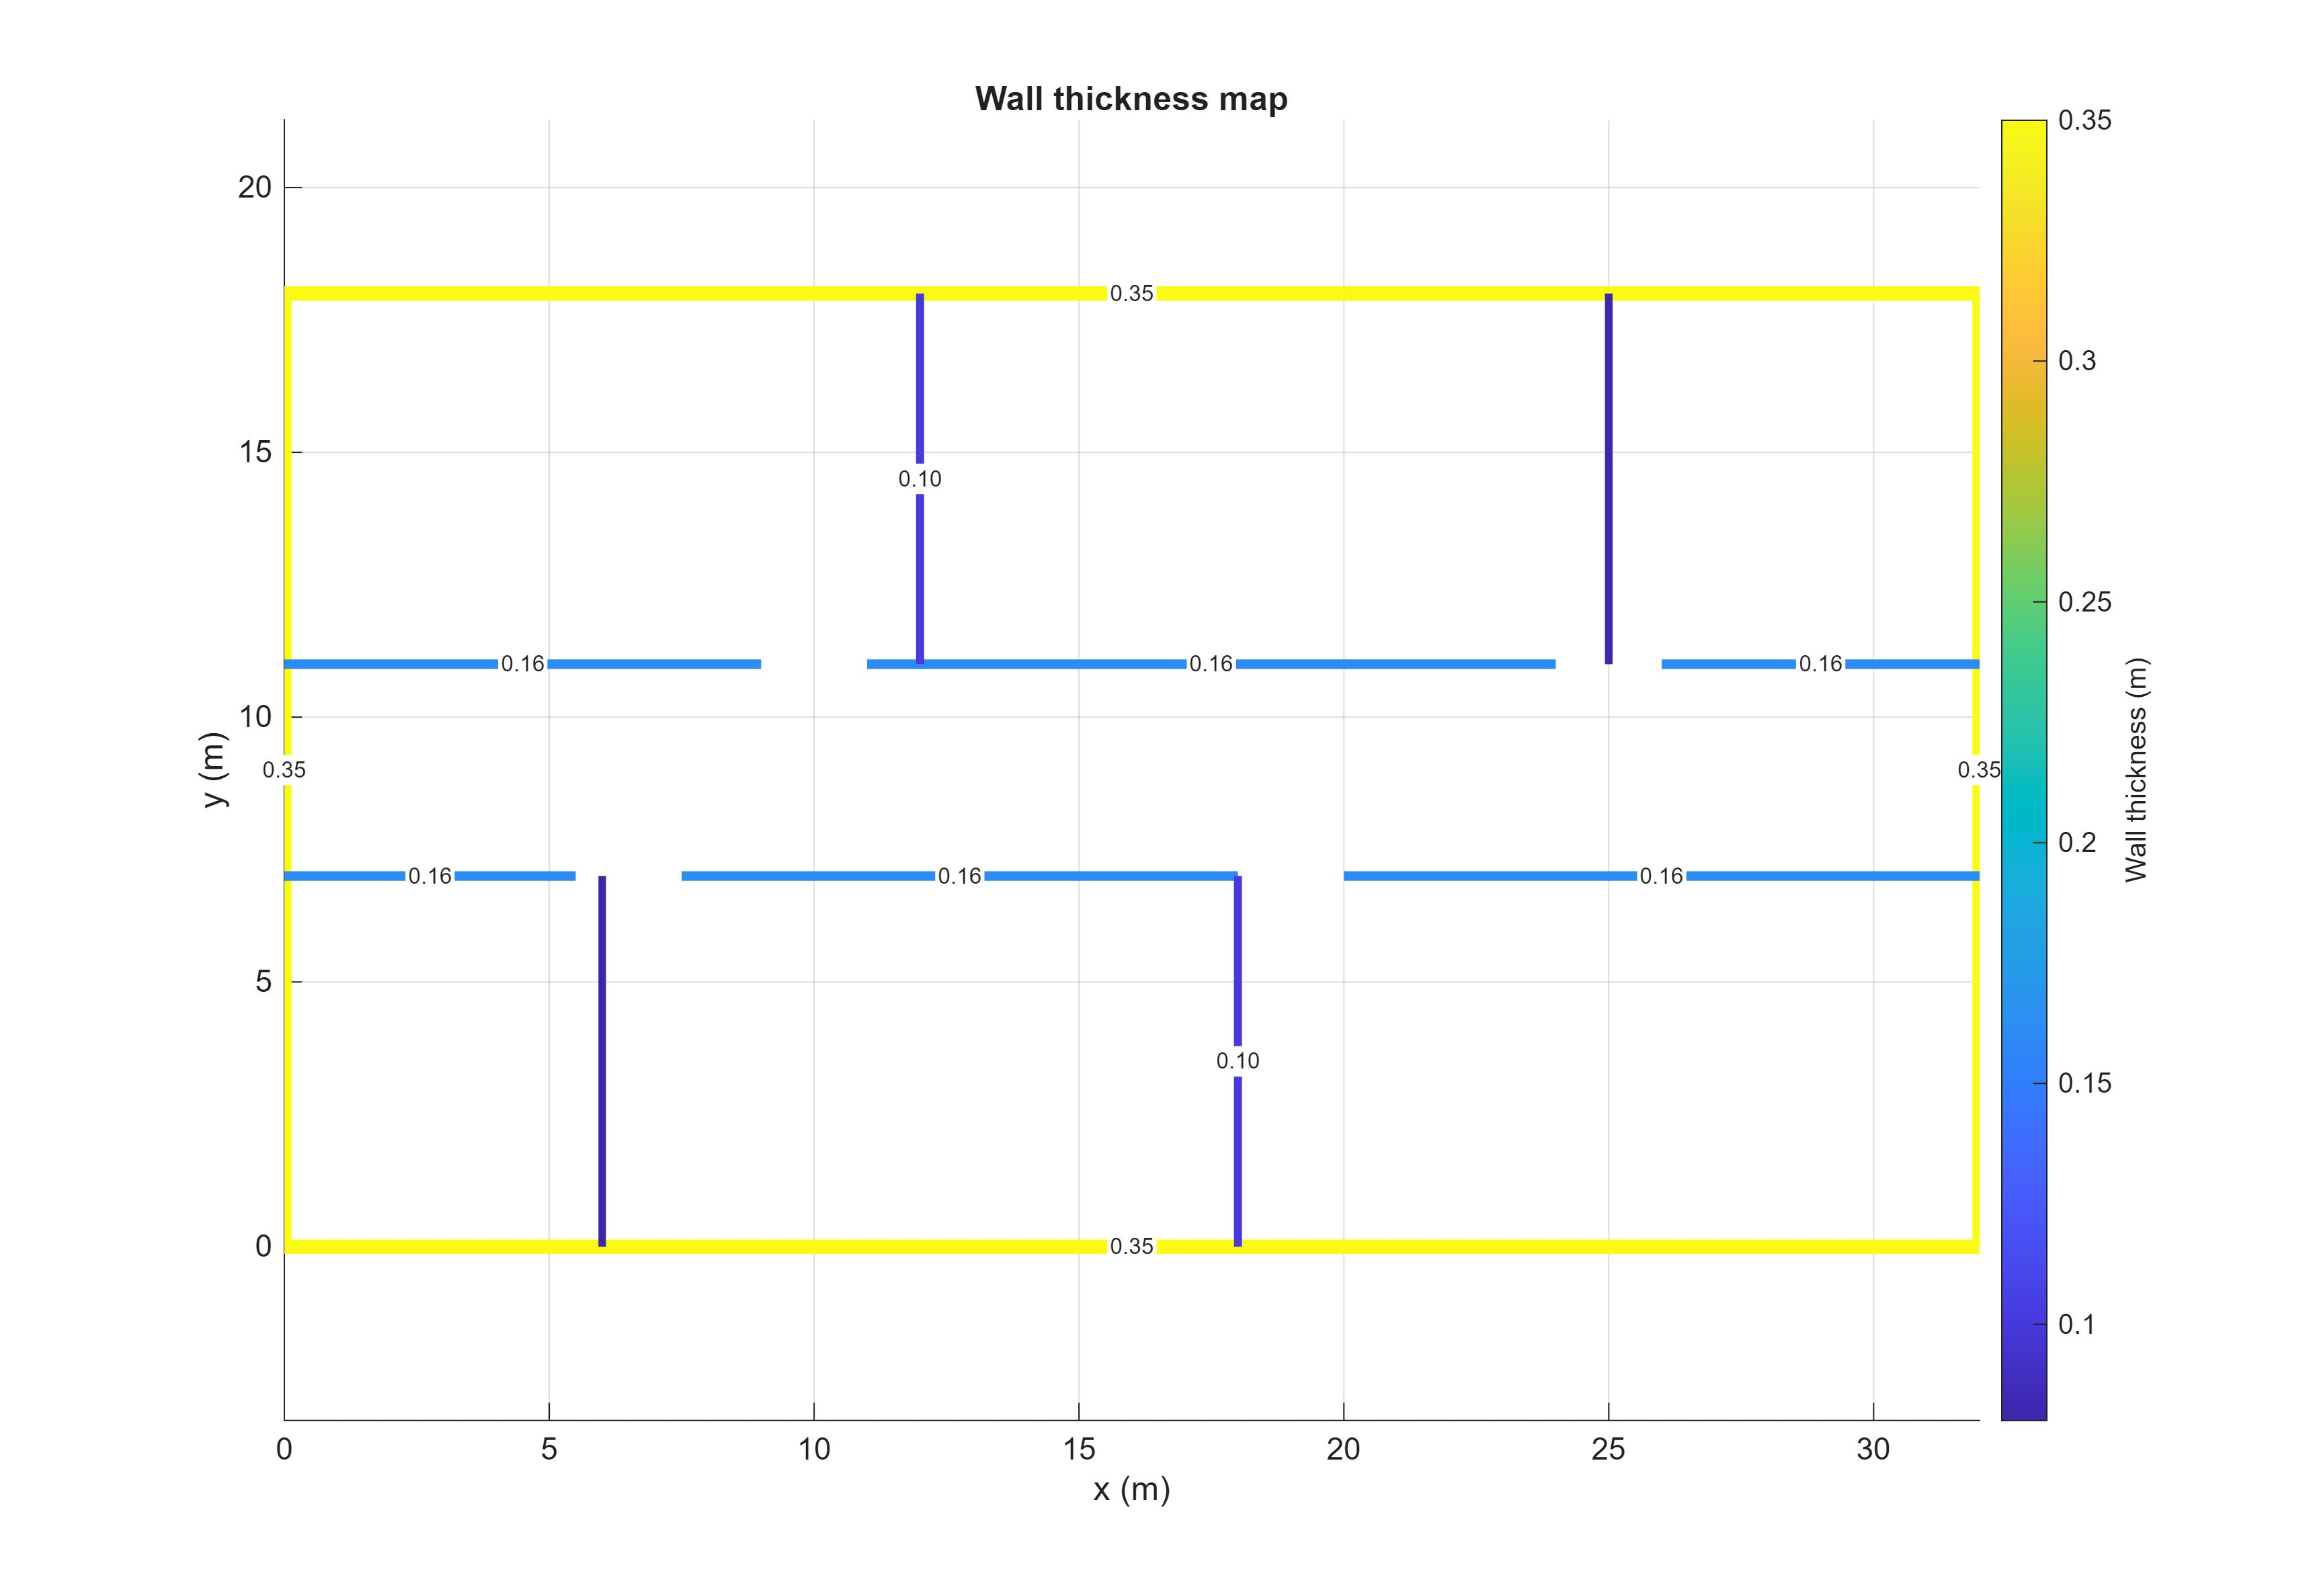
\includegraphics[width=0.30\textwidth]{scenario_001_fig_map_wall_thickness.png} &
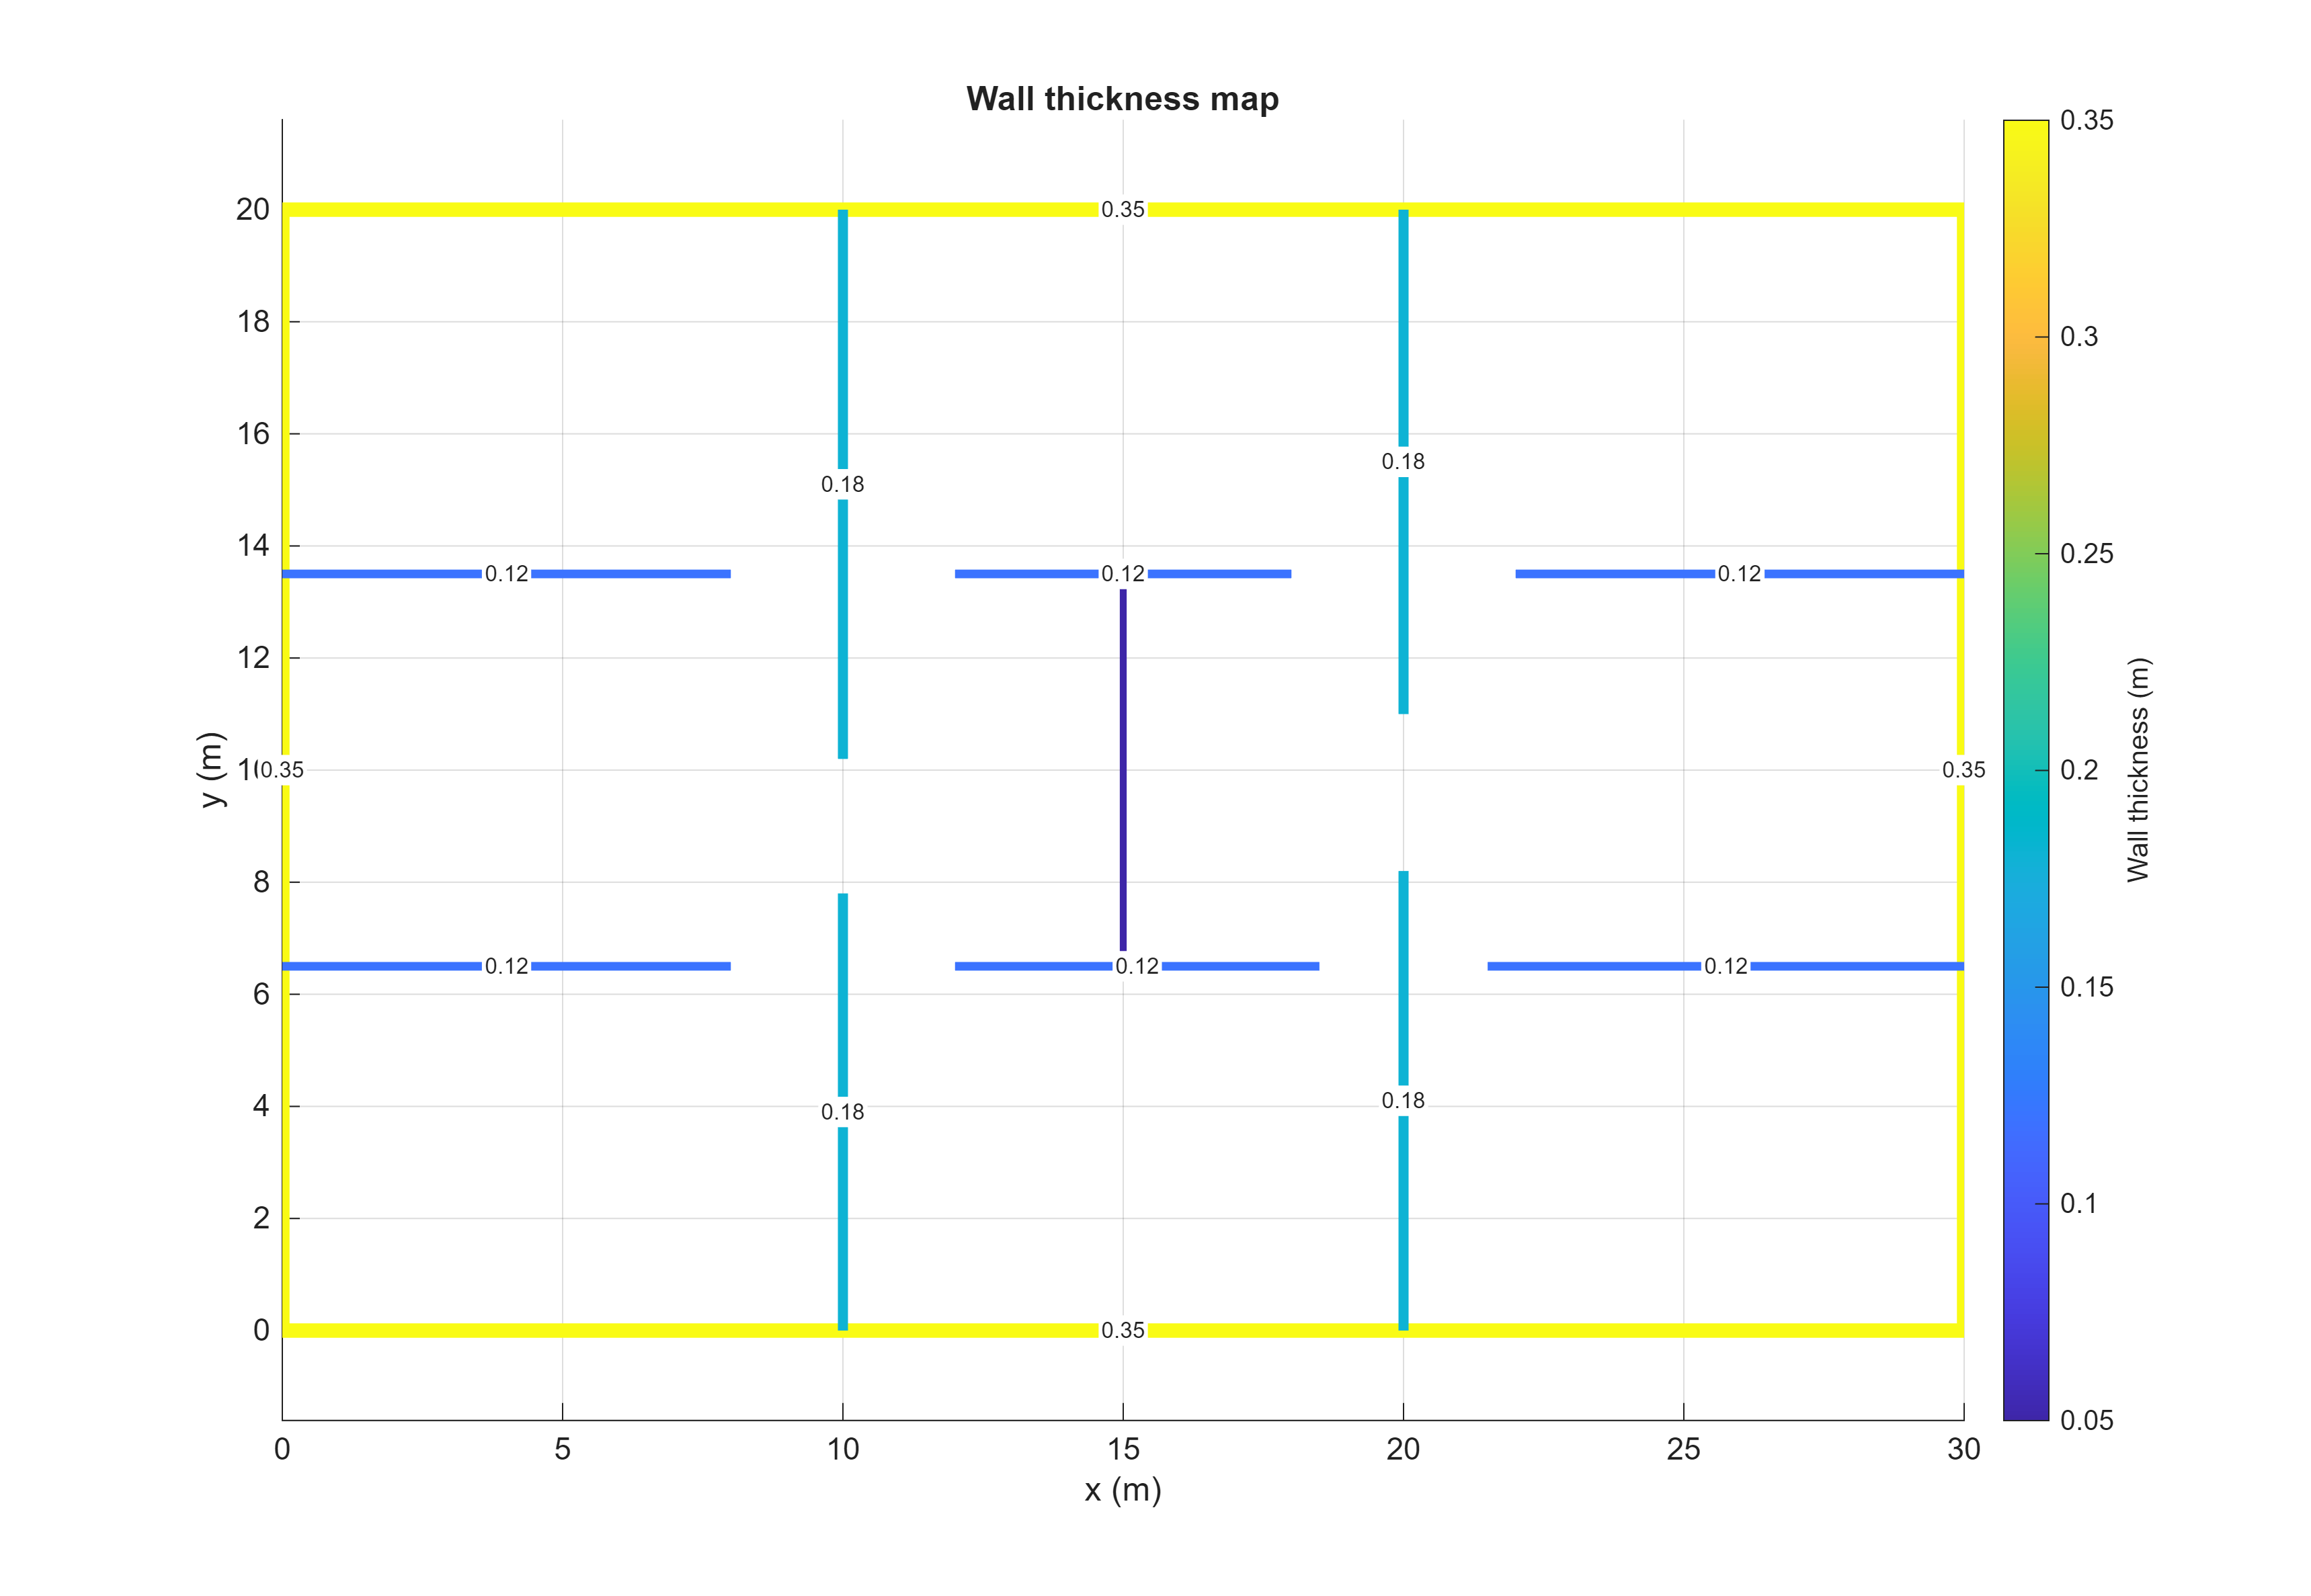
\includegraphics[width=0.30\textwidth]{scenario_002_fig_map_wall_thickness.png} &
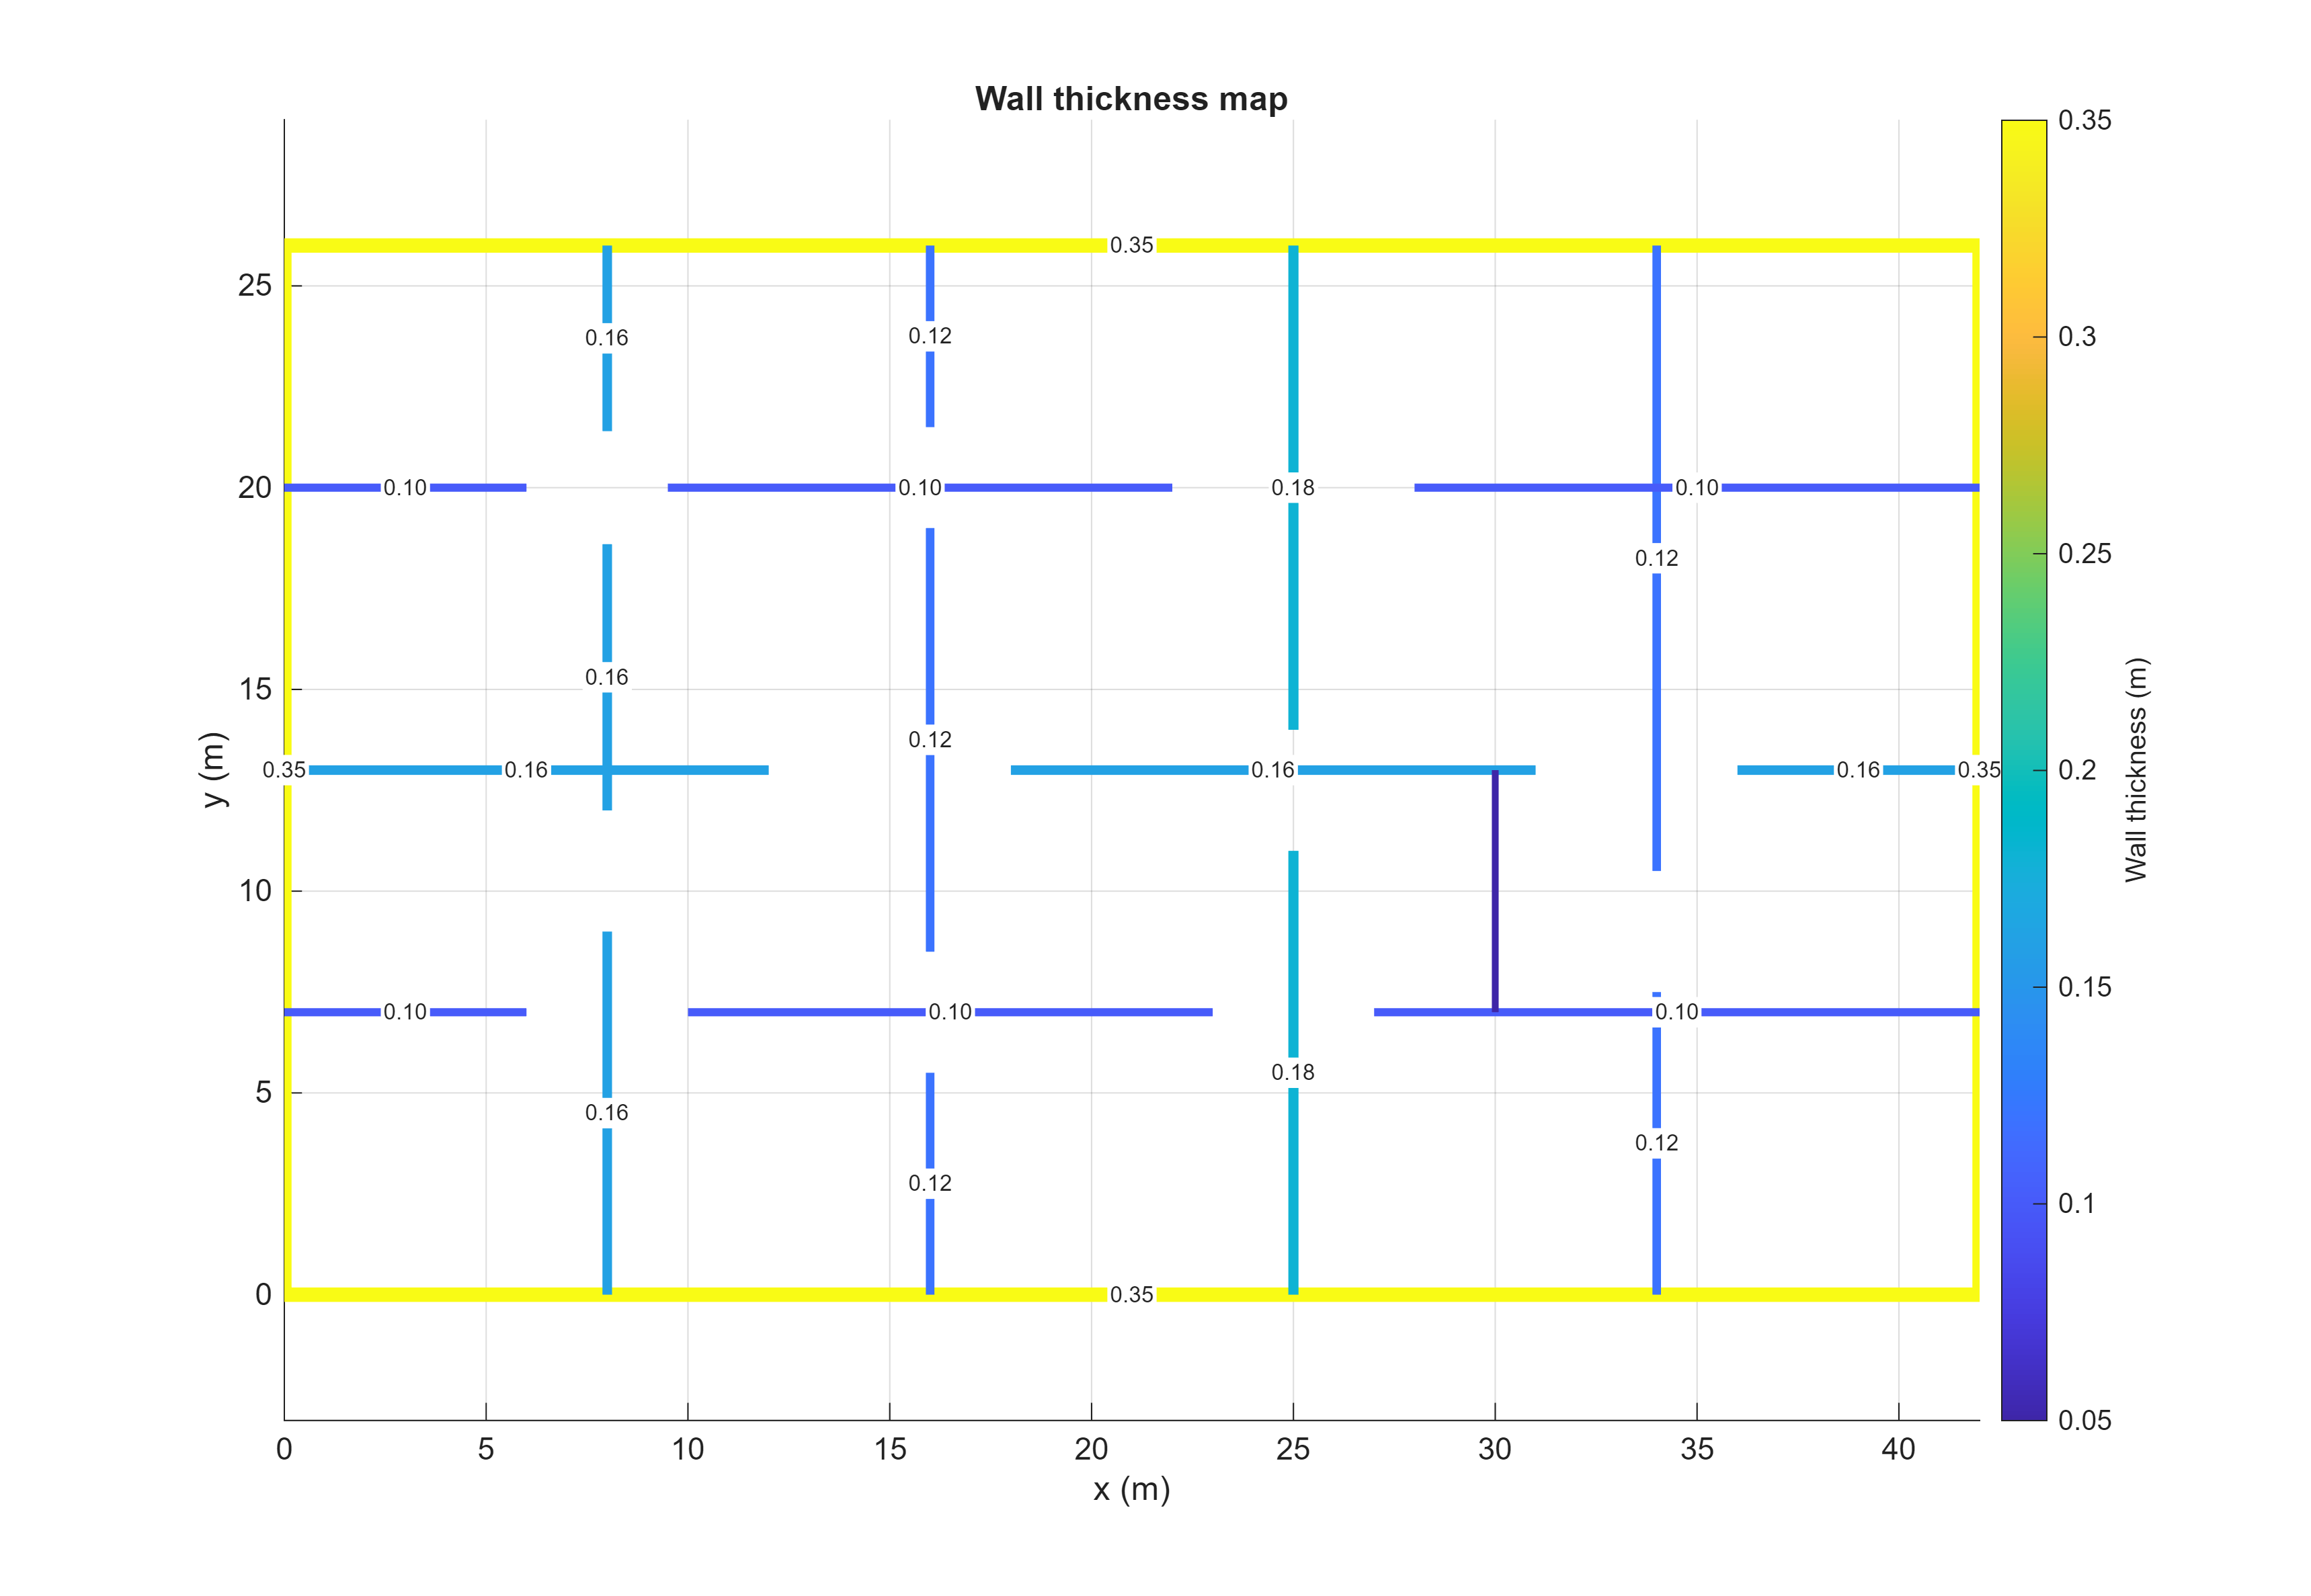
\includegraphics[width=0.30\textwidth]{scenario_003_fig_map_wall_thickness.png}\\
(a) Scenario 1 & (b) Scenario 2 & (c) Scenario 3
\end{tabular}
\caption{Generated wall-segment maps with wall thickness metadata. The three map types are an open hallway with side rooms, a multi-room layout, and a larger dense indoor map.}
\label{fig:scenario_layouts}
\end{figure*}

\begin{figure*}
\centering
\begin{tabular}{ccc}
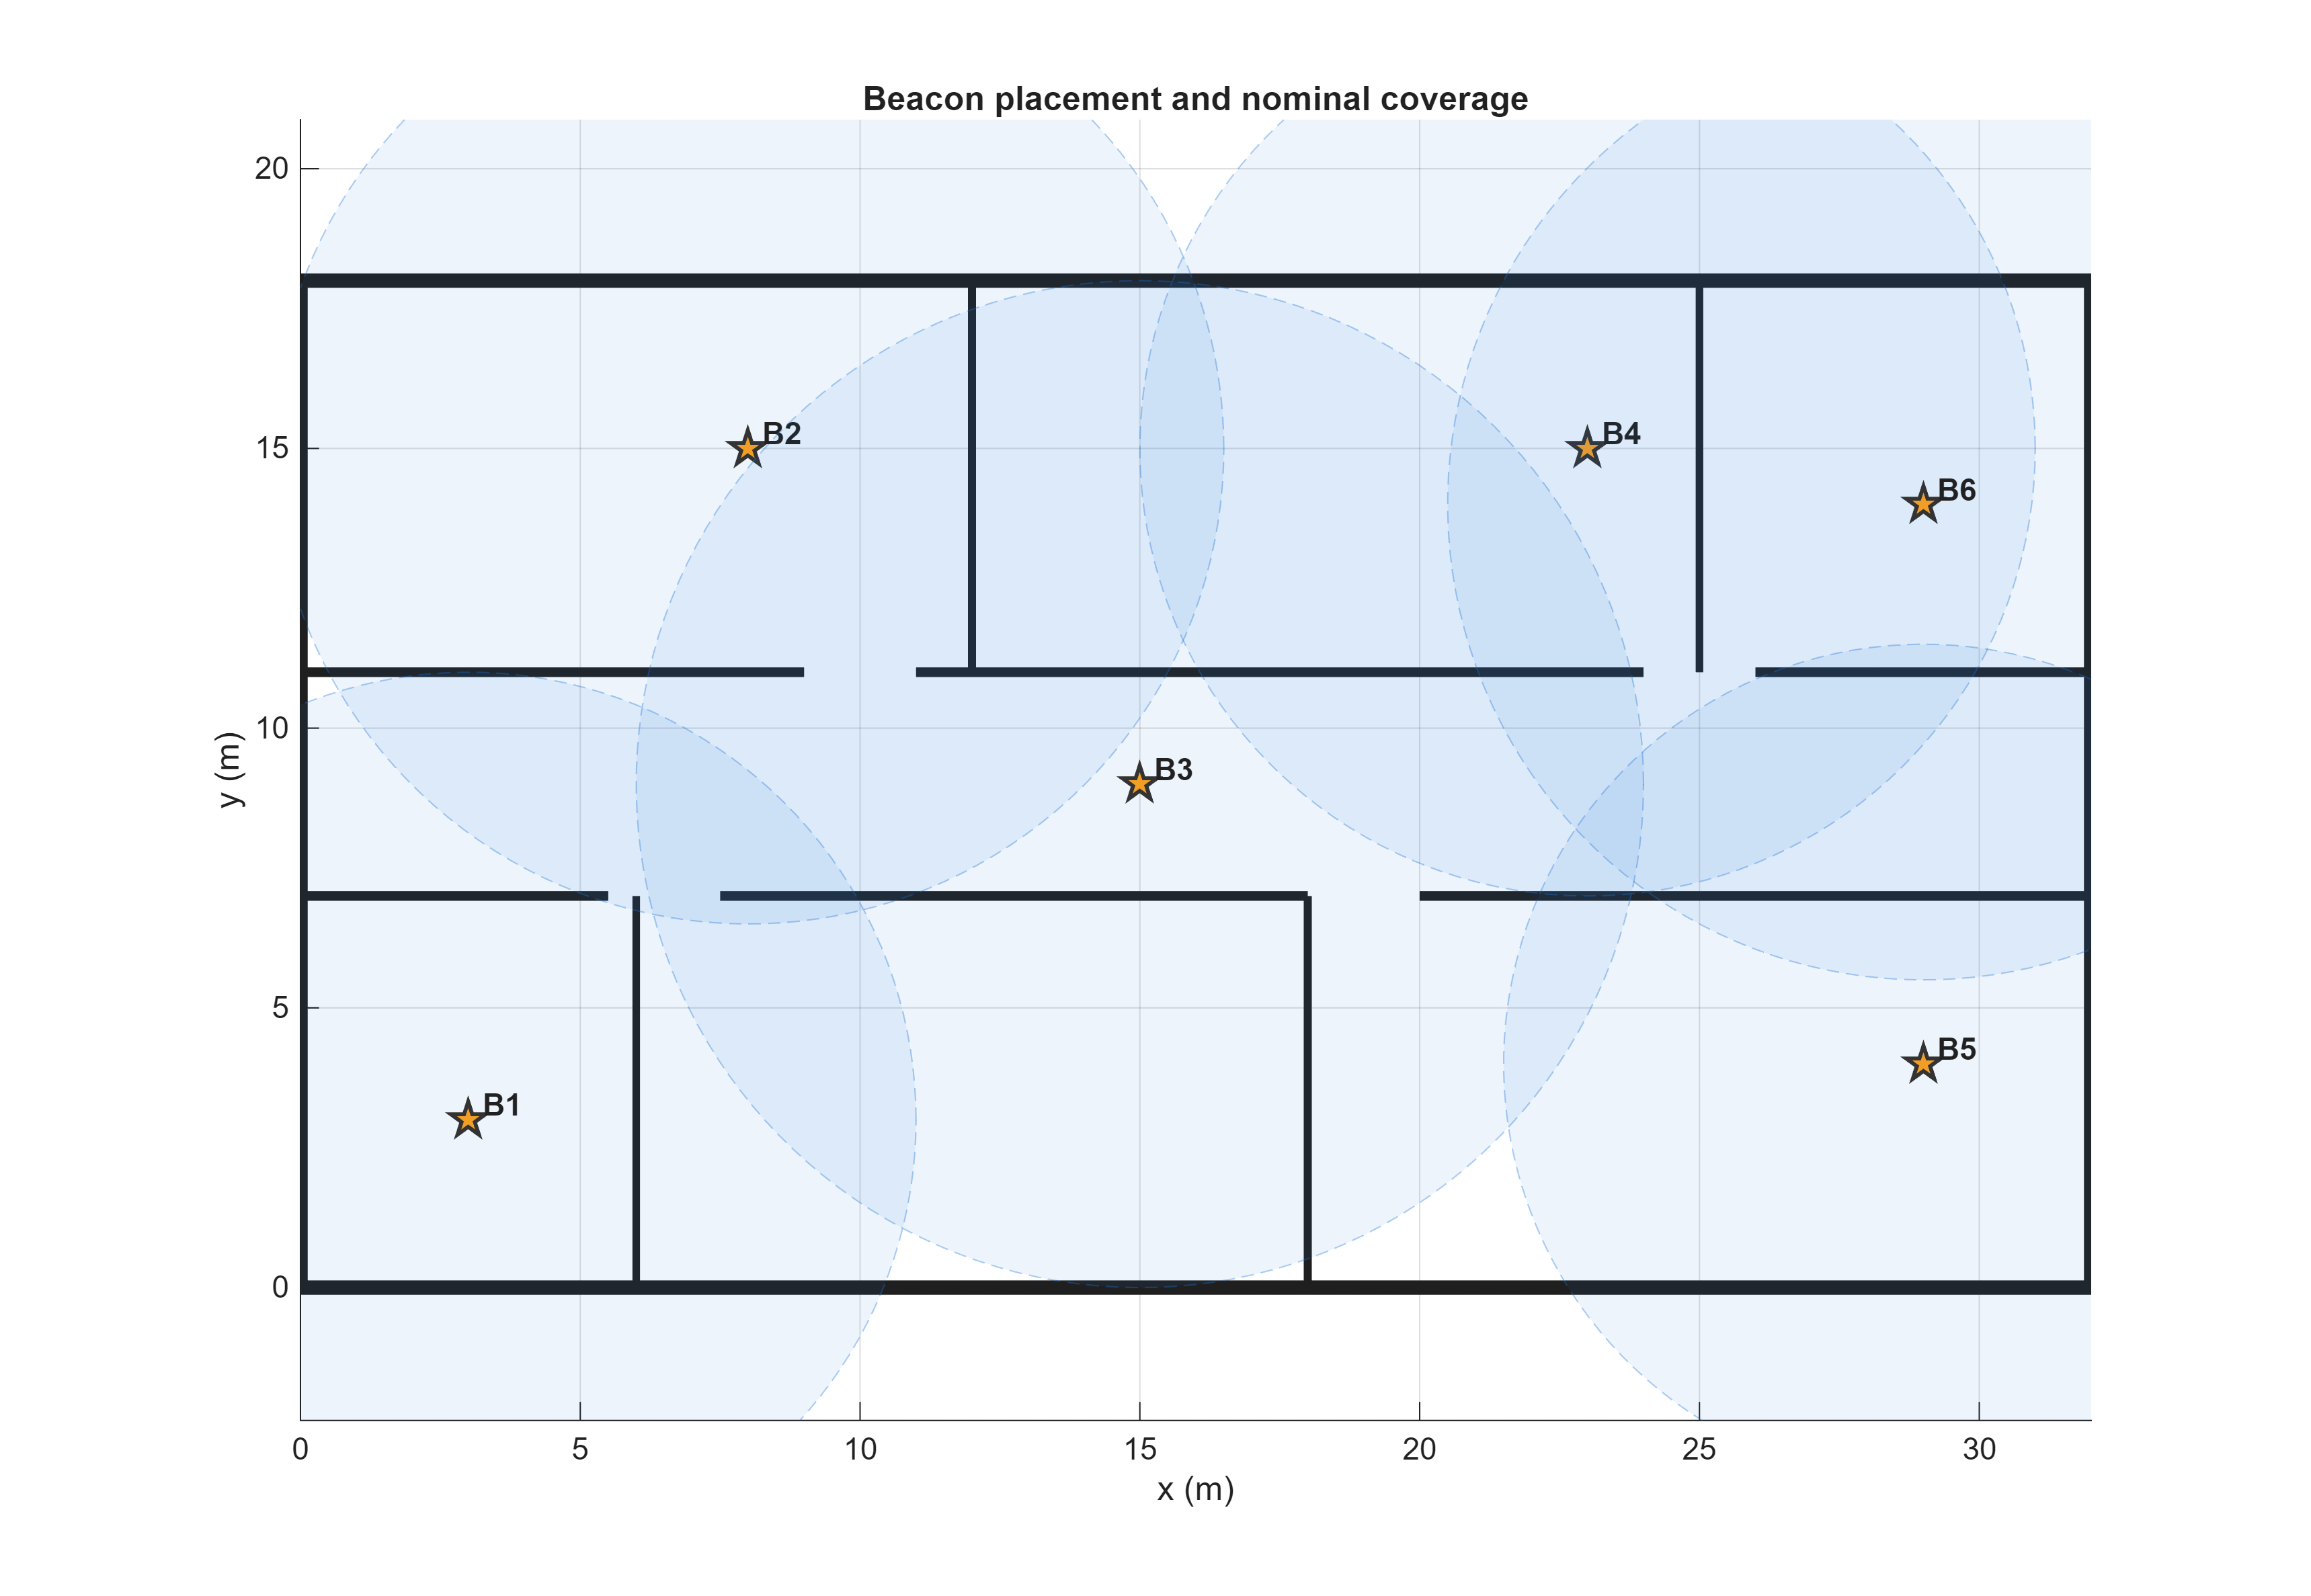
\includegraphics[width=0.30\textwidth]{scenario_001_fig_beacon_layout.png} &
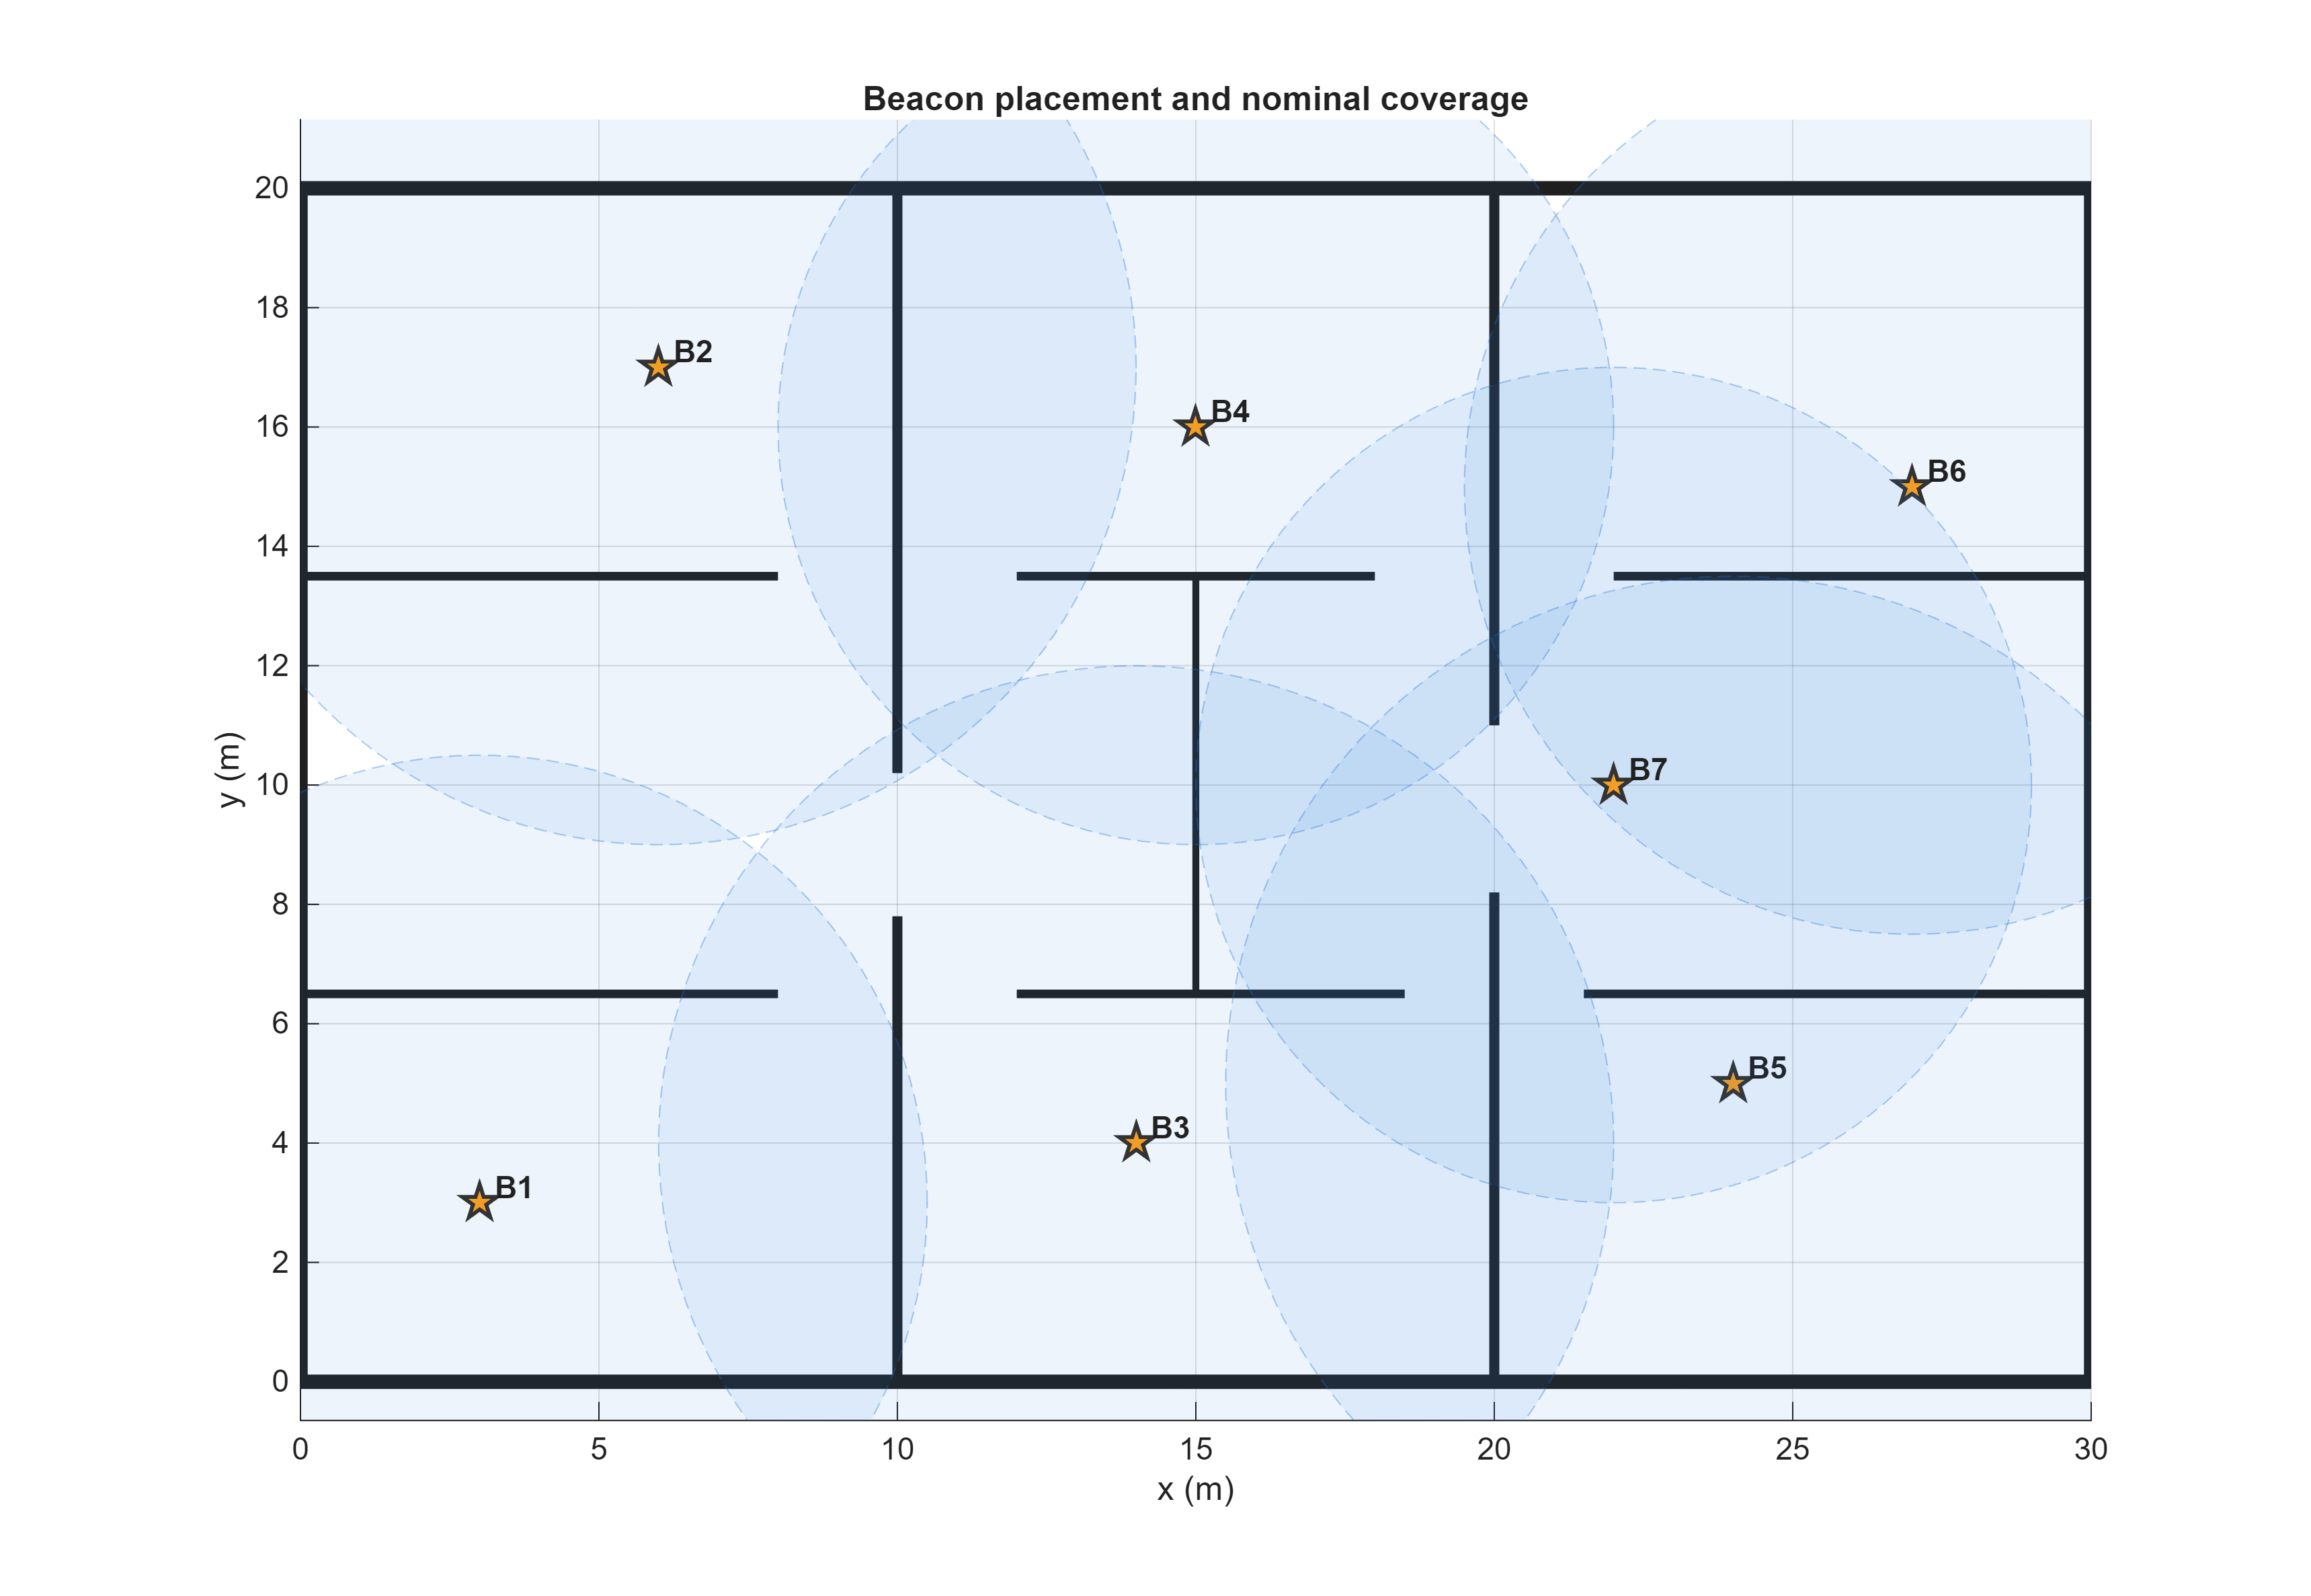
\includegraphics[width=0.30\textwidth]{scenario_002_fig_beacon_layout.png} &
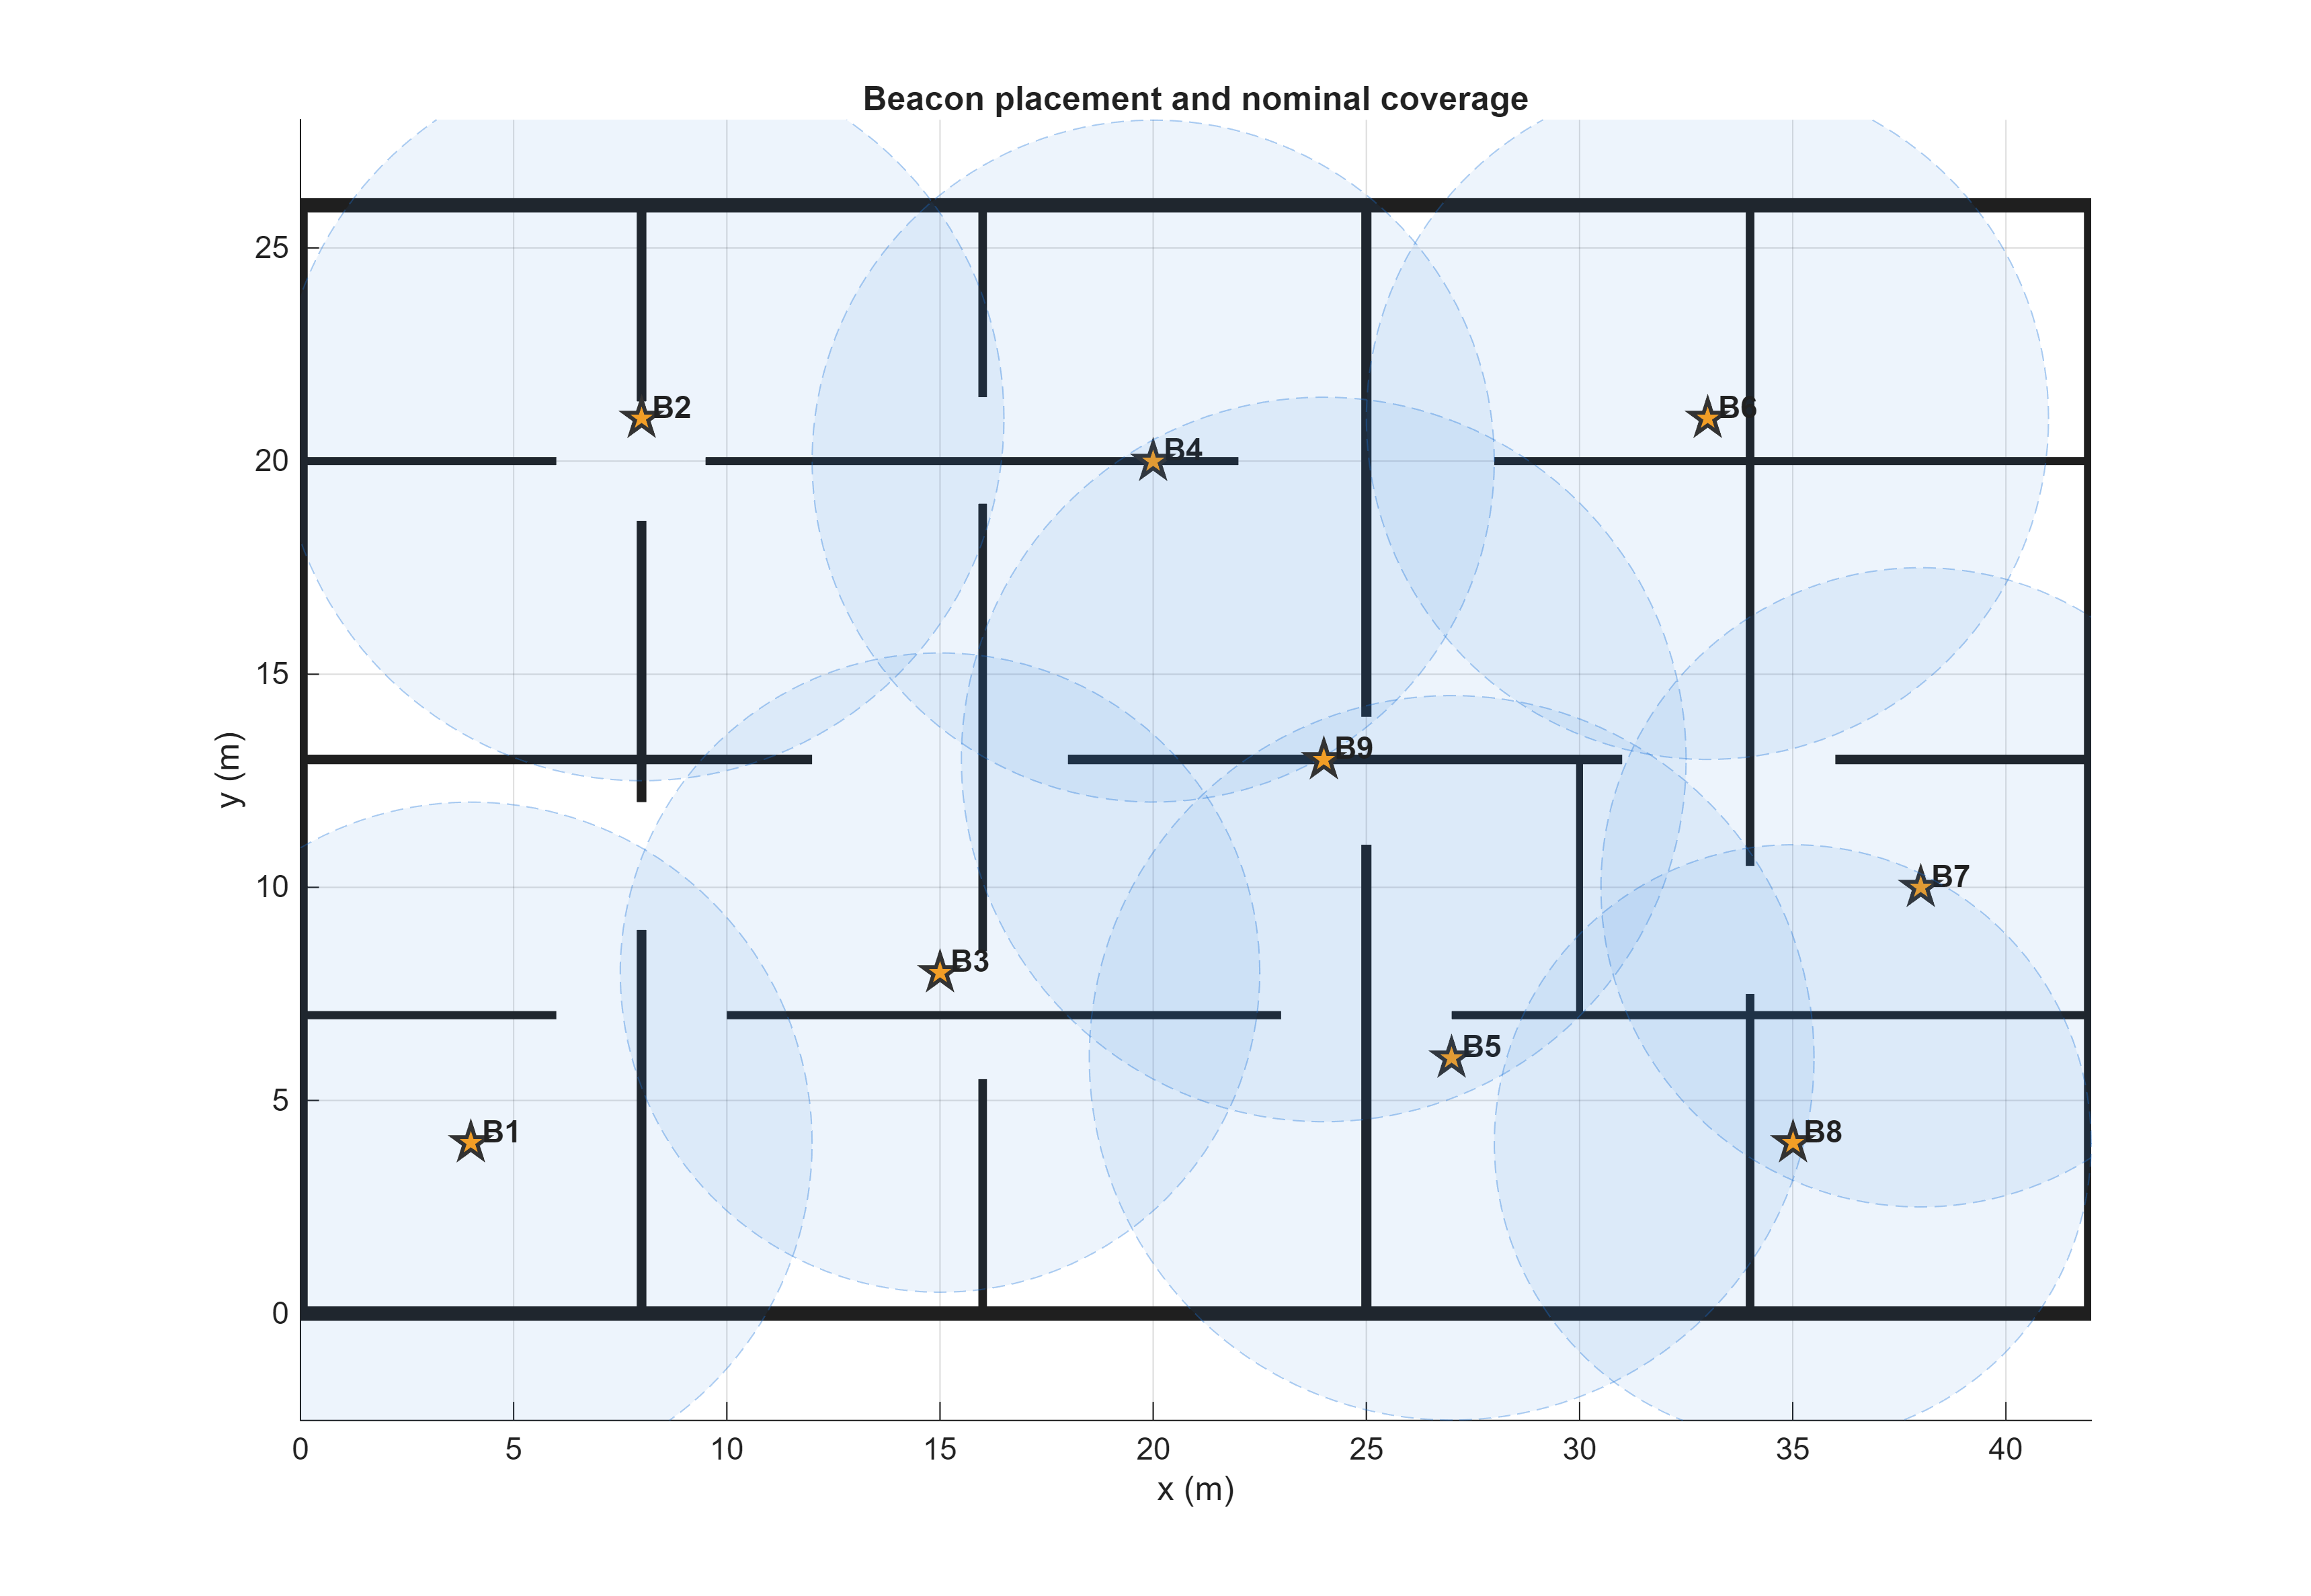
\includegraphics[width=0.30\textwidth]{scenario_003_fig_beacon_layout.png}\\
(a) Scenario 1 & (b) Scenario 2 & (c) Scenario 3
\end{tabular}
\caption{Beacon placements and nominal coverage regions for the three saved scenarios. Beacon range limits and penetration budgets are scenario-specific configuration parameters.}
\label{fig:beacon_layouts}
\end{figure*}

\begin{figure*}
\centering
\begin{tabular}{ccc}
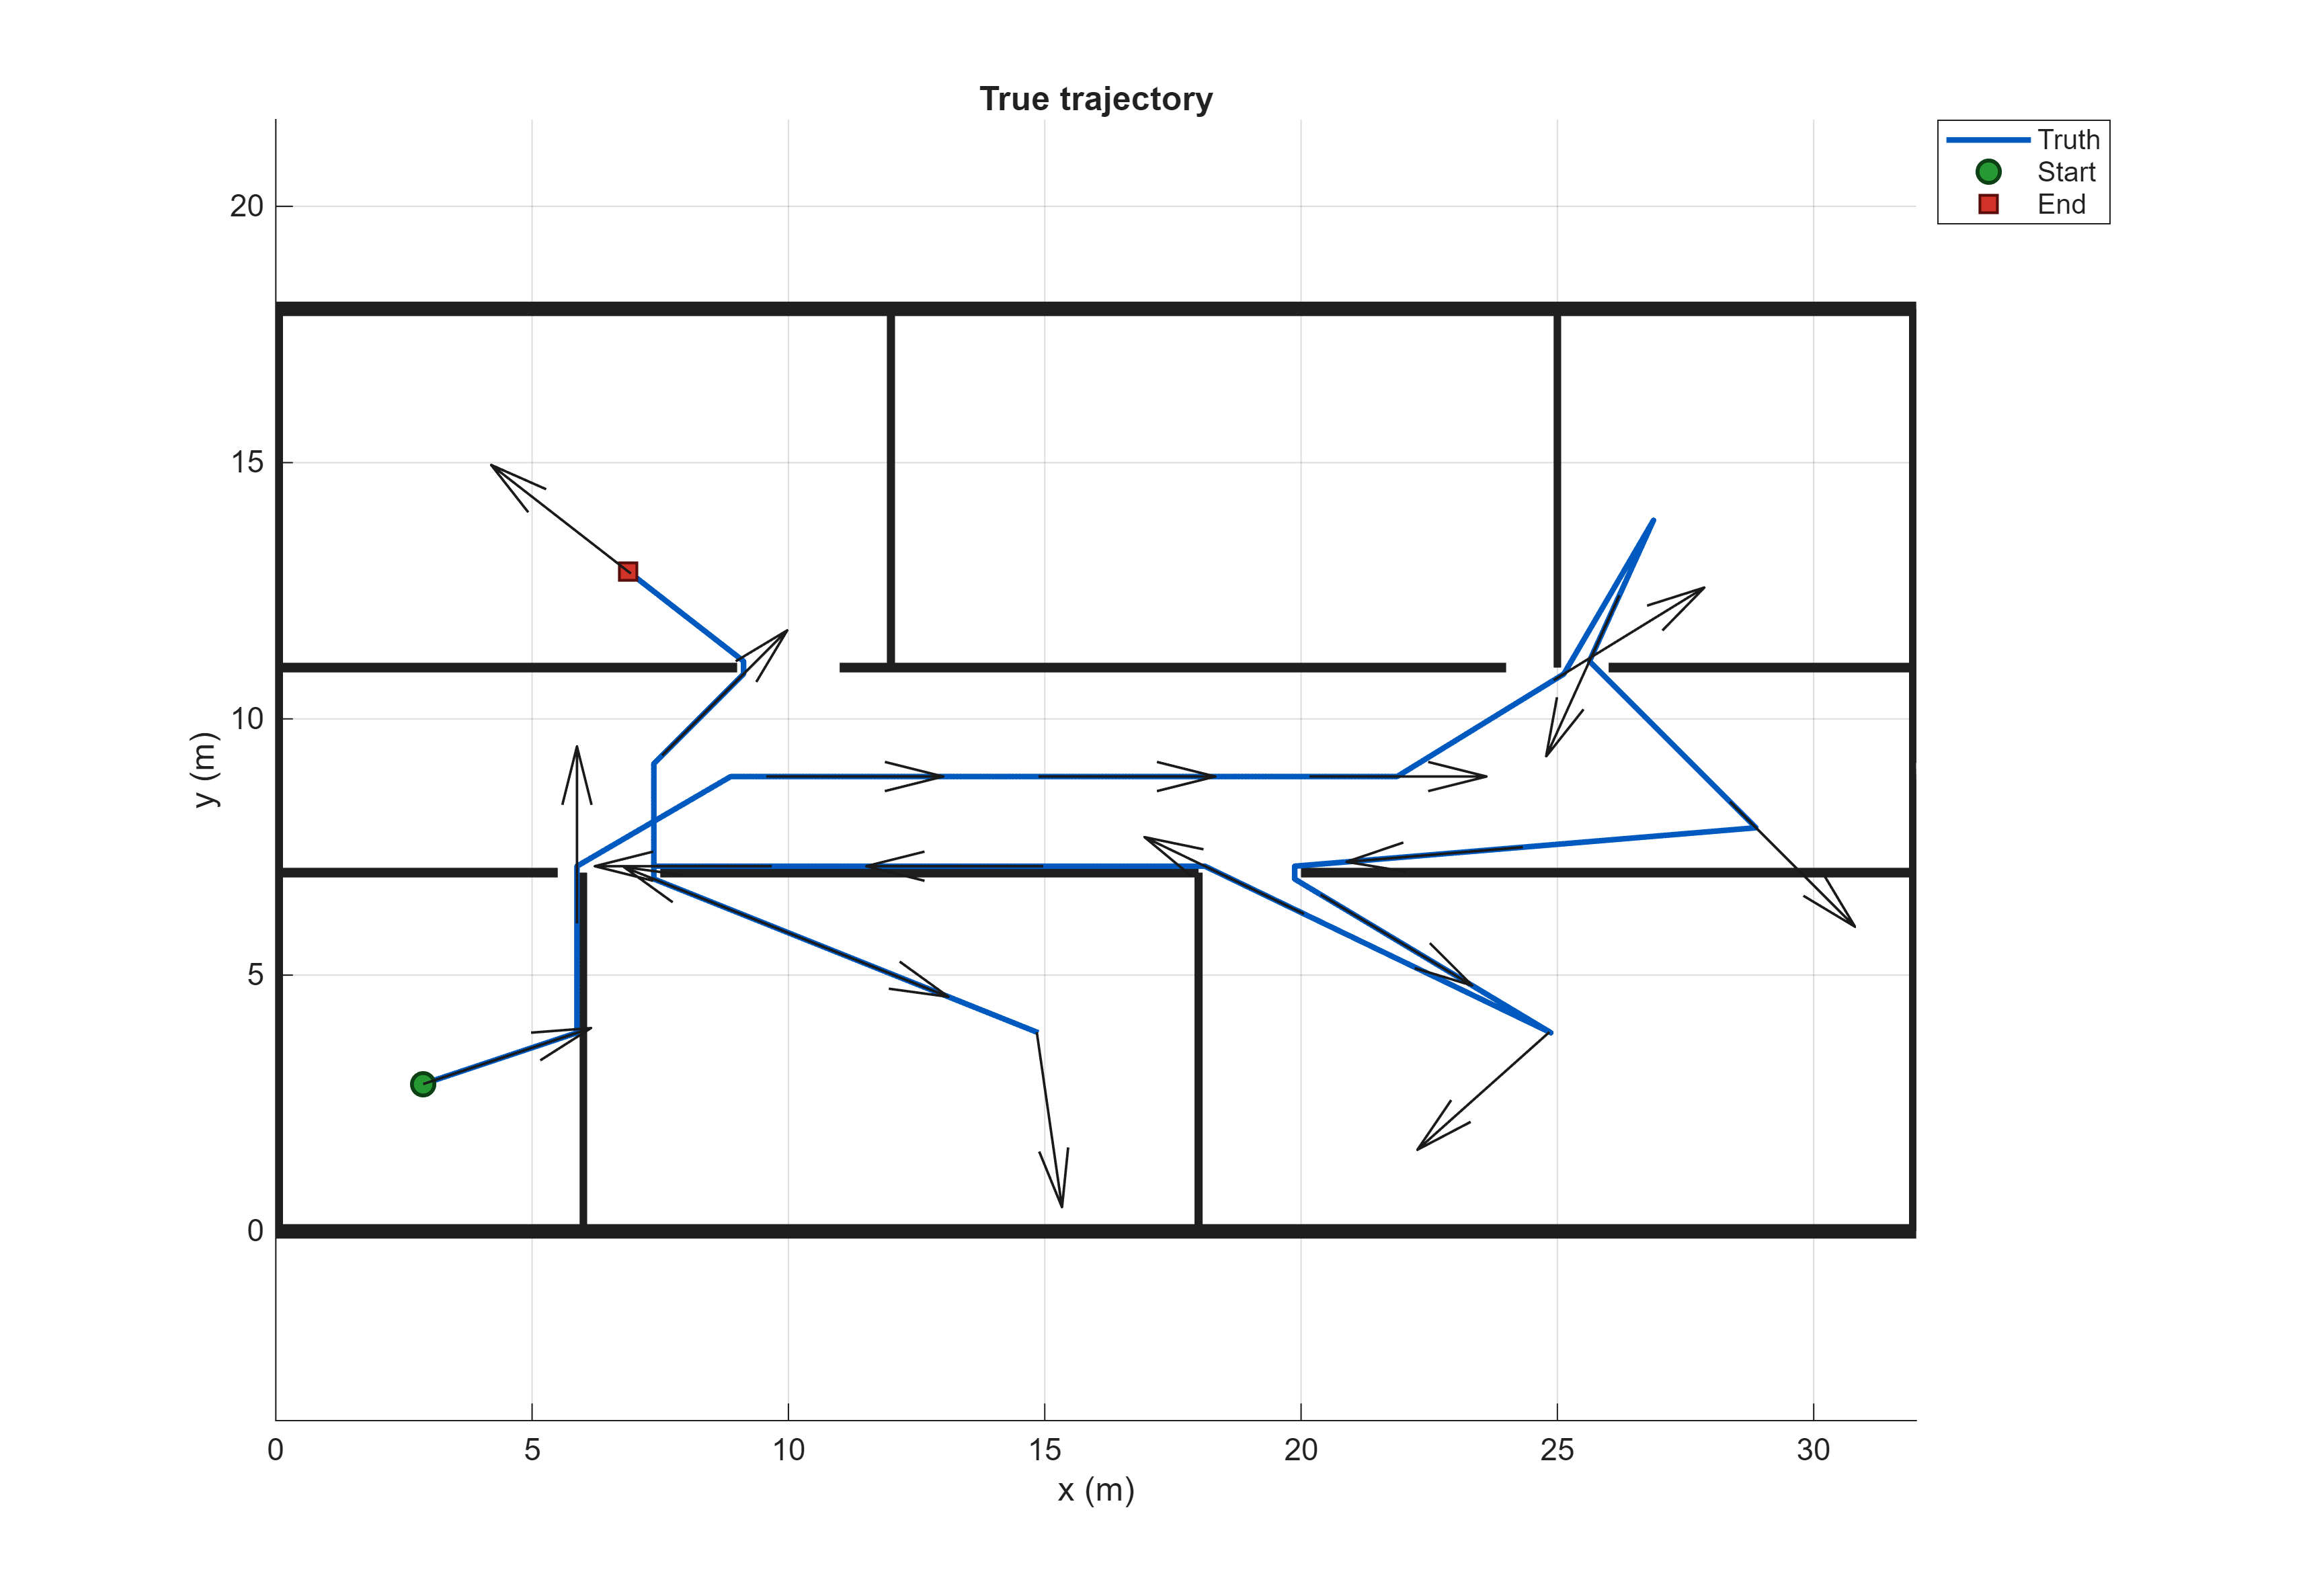
\includegraphics[width=0.30\textwidth]{scenario_001_fig_true_trajectory.png} &
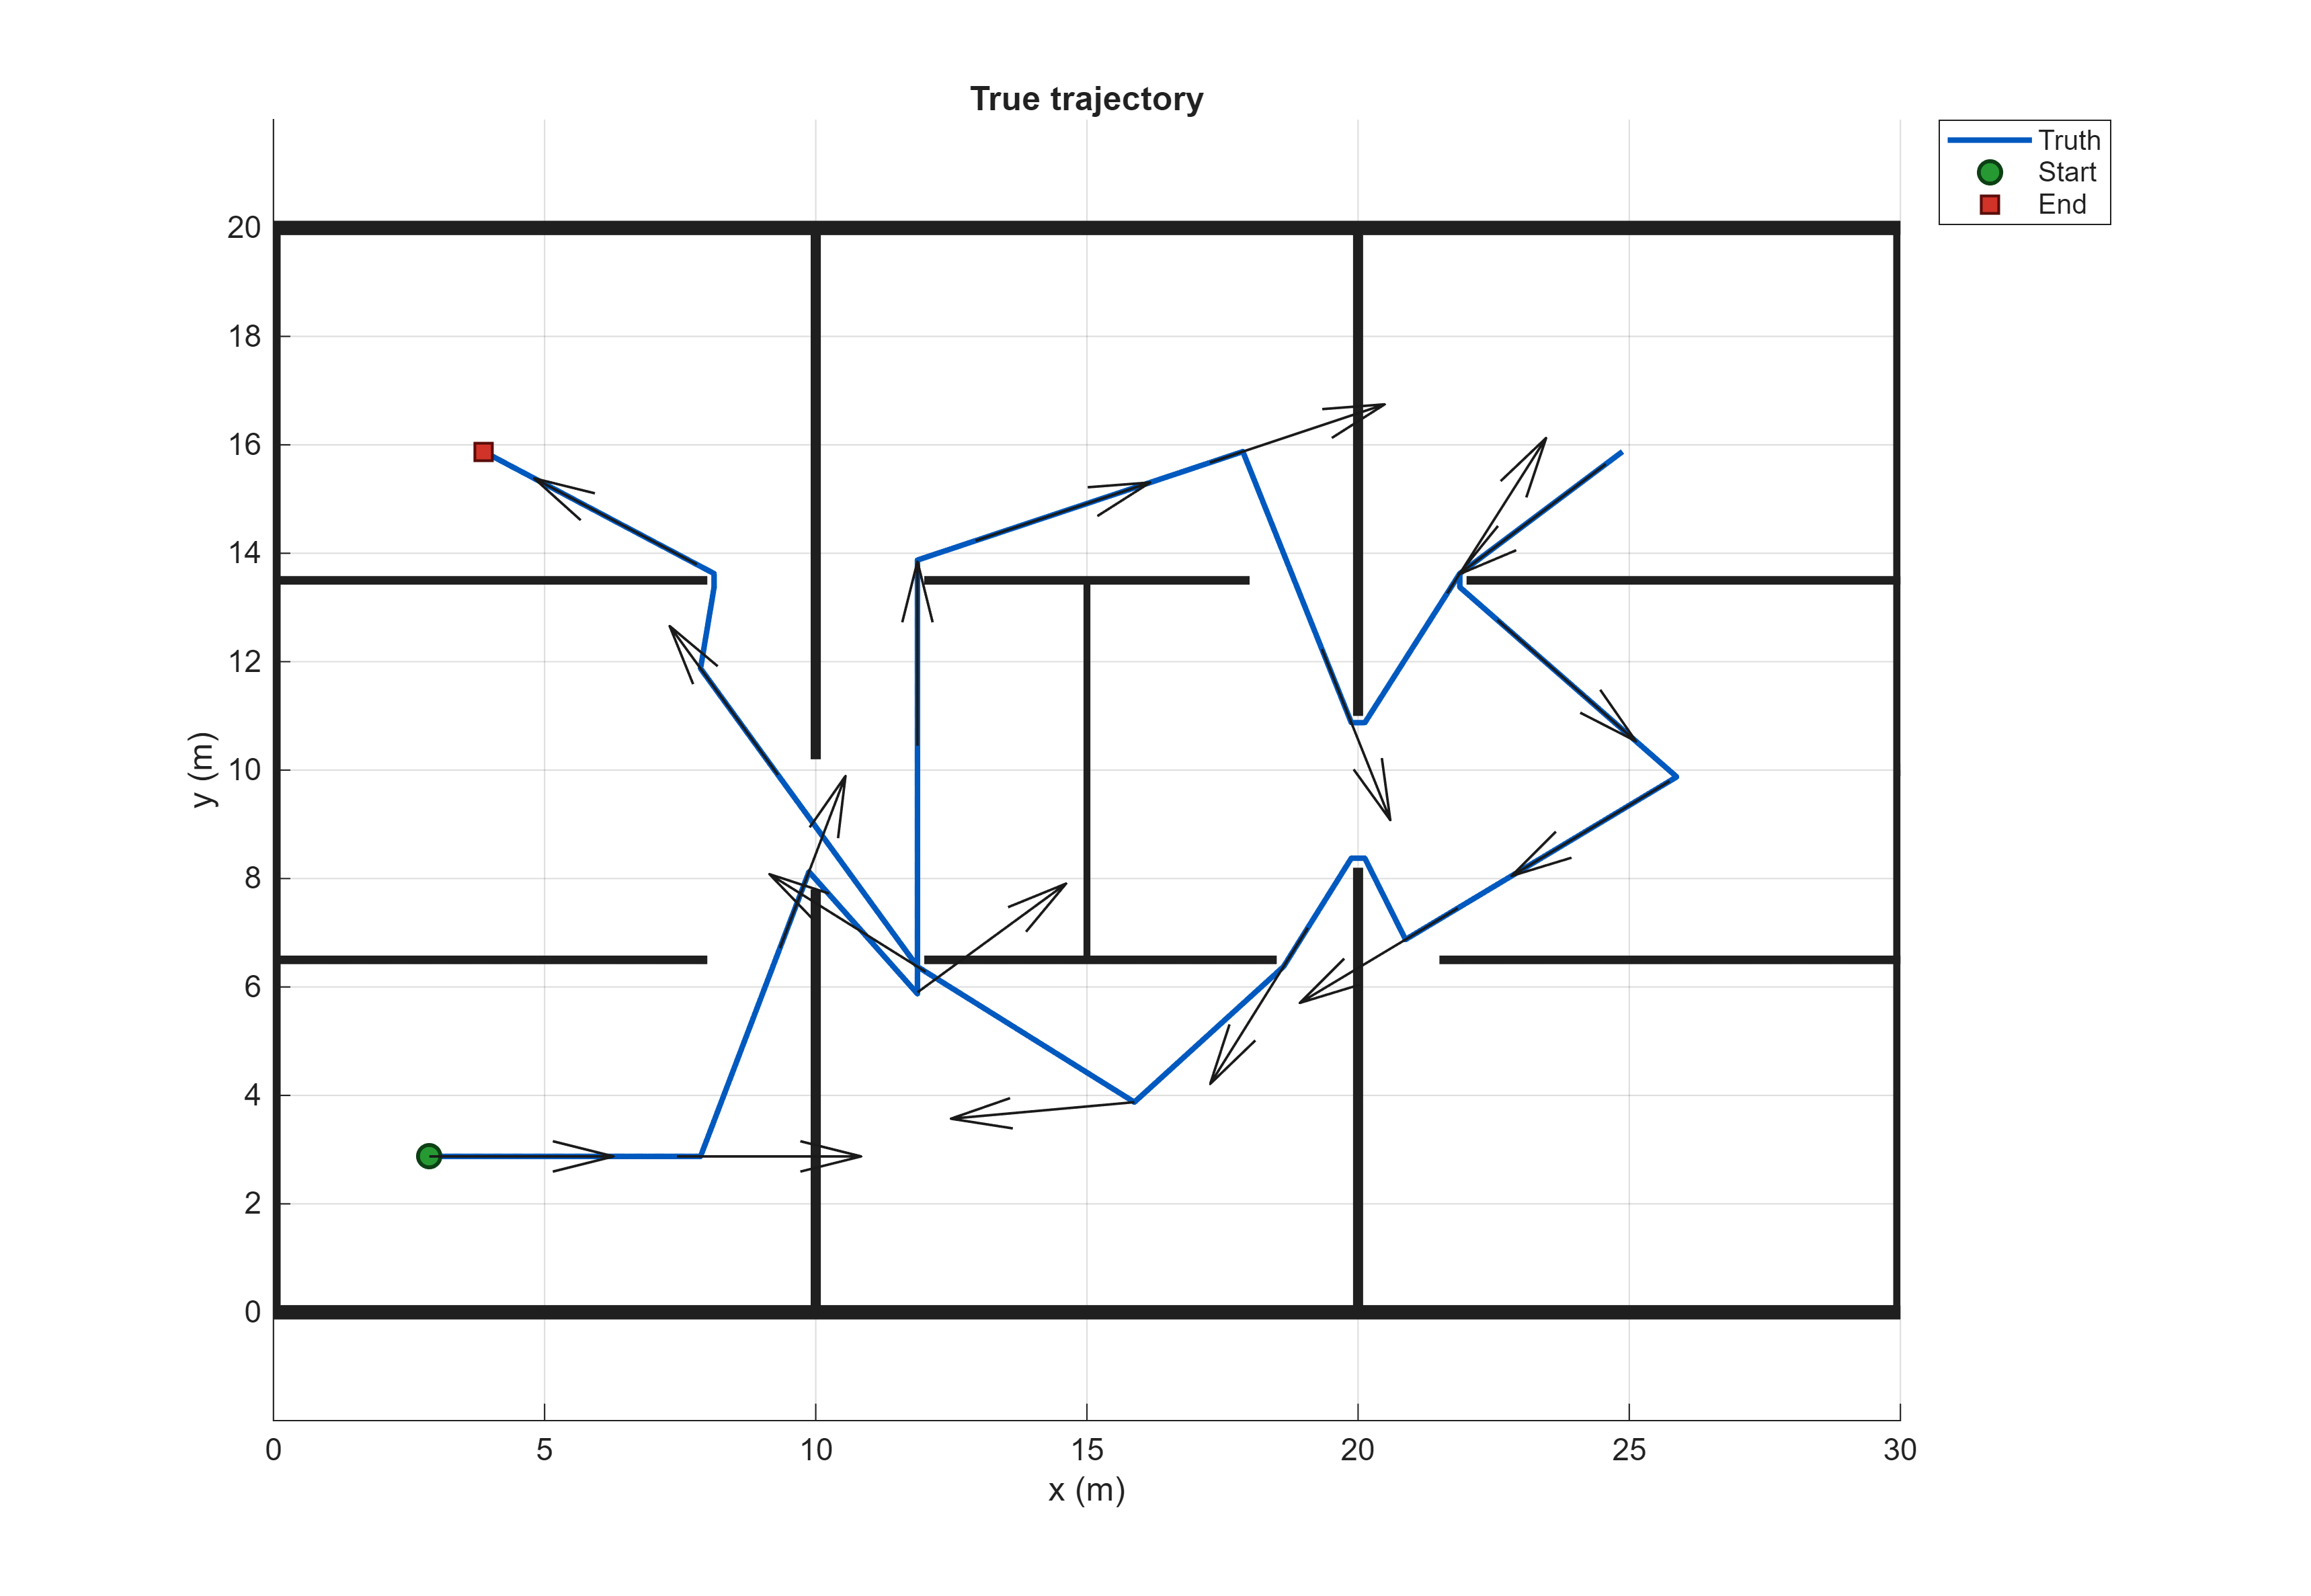
\includegraphics[width=0.30\textwidth]{scenario_002_fig_true_trajectory.png} &
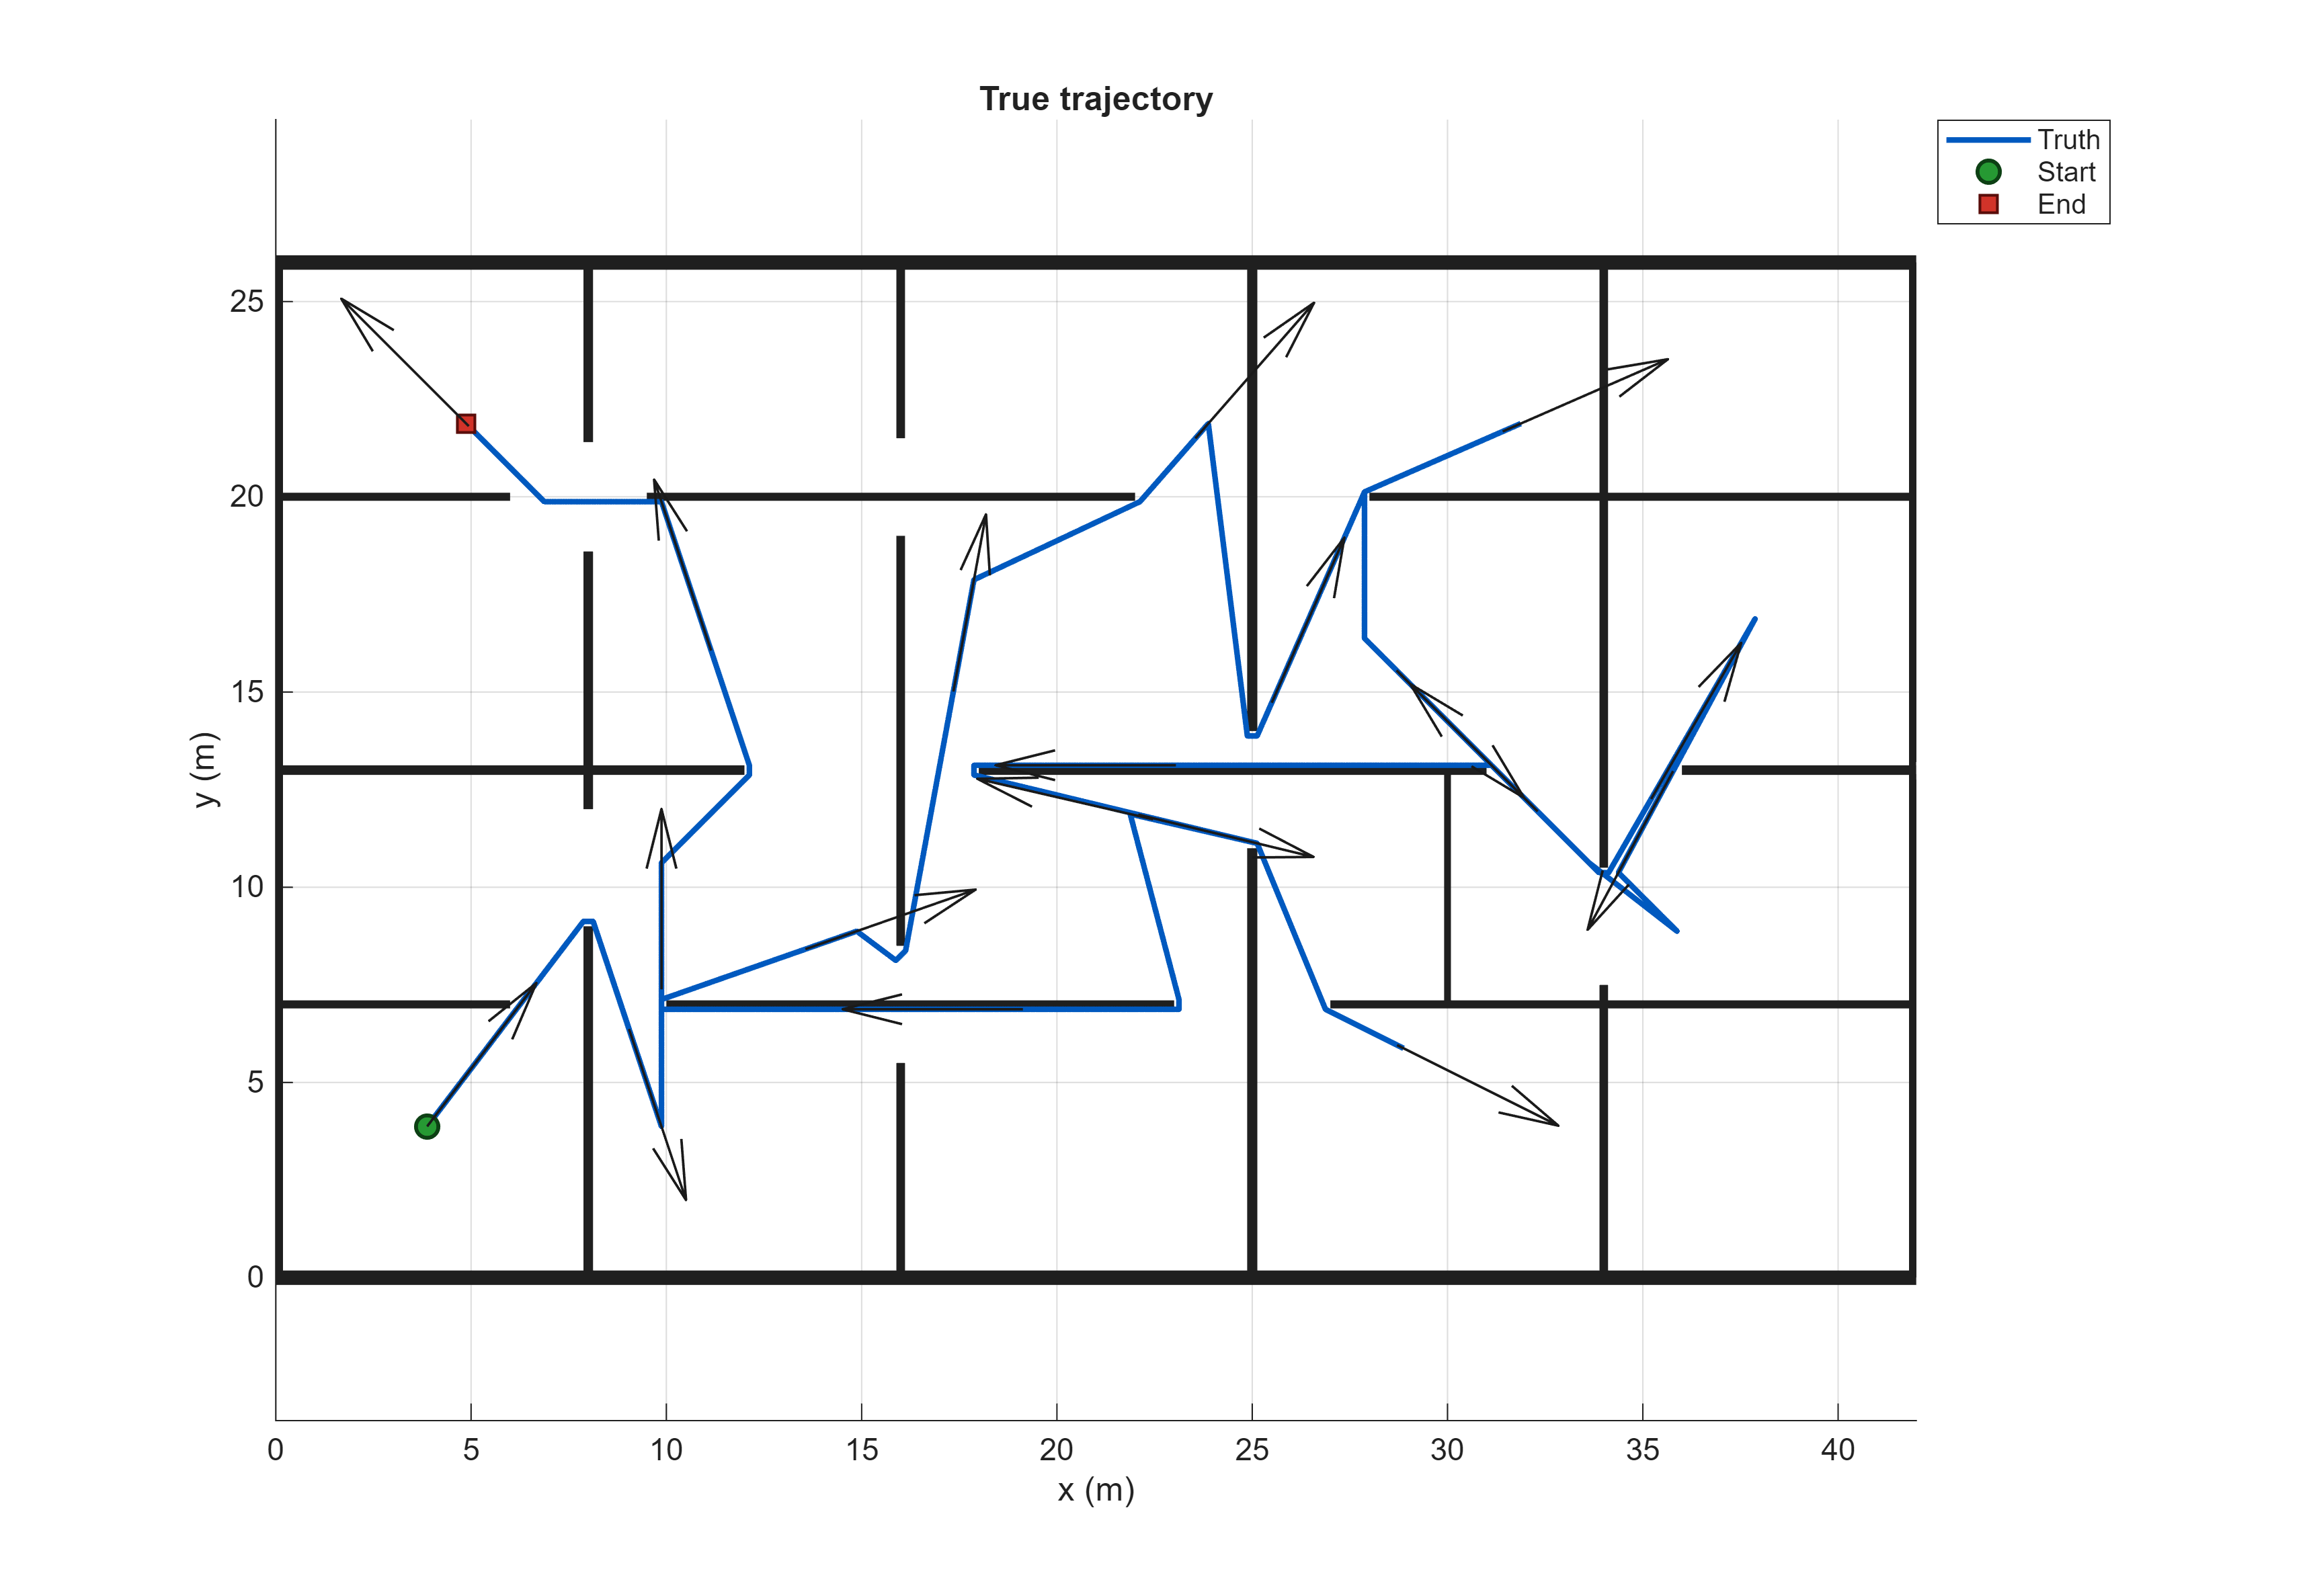
\includegraphics[width=0.30\textwidth]{scenario_003_fig_true_trajectory.png}\\
(a) Scenario 1 & (b) Scenario 2 & (c) Scenario 3
\end{tabular}
\caption{Saved ground-truth trajectories. Requested waypoints are routed through wall openings by the wall-aware planner, and saved trajectories are rejected if sampled segments intersect walls.}
\label{fig:true_trajectories}
\end{figure*}

\subsection{Map Structure}

Each map begins with four outer boundary walls of thickness 0.35 m and material factor 2.4. Interior walls are then added according to the scenario type. The open hallway scenario contains horizontal hallway walls and vertical room partitions. The multi-room scenario contains two main vertical interior walls, horizontal partitions, and one glass divider. The large dense scenario expands the bounds and adds multiple vertical and horizontal partitions, plus an explicit upper doorway aligned with the north-corridor return leg.

\subsection{Beacon Setup}

Beacon positions, maximum ranges, and penetration budgets are scenario-specific. Scenario 1 uses six beacons with maximum ranges from 7.5 m to 9.0 m and penetration budgets from 0.25 to 0.36. Scenario 2 uses seven beacons with maximum ranges from 7.0 m to 8.5 m and budgets from 0.20 to 0.32. Scenario 3 uses nine beacons with maximum ranges from 7.0 m to 8.5 m and budgets from 0.18 to 0.28. The common RSSI threshold is \(-82\) dB, and the random dropout probability is \(0.04\) multiplied by the scenario dropout scale in Table~\ref{tab:scenarios}.

\subsection{LiDAR and Prediction Setup}

The LiDAR field of view is \(270^\circ\), with 181 beams and a 12 m maximum range. Each scan must have at least 25 valid returns for a pose measurement to be considered available, and the scan quality must exceed 0.18. The LiDAR random dropout probability is \(0.03\) multiplied by the scenario dropout scale.

The prediction input is generated from the saved trajectory by differentiating velocity for world-frame acceleration, rotating it into the body frame, and differentiating unwrapped heading for yaw rate. Noisy body acceleration and yaw rate are saved in \texttt{prediction\_inputs.mat}. The filter initializes the nominal state from the first saved truth state and uses the configured initial covariance
\begin{equation}
P_0=\diag\left((4^\circ)^2,0.25^2,0.25^2,0.18^2,0.18^2\right).
\end{equation}

\begin{figure*}
\centering
\begin{tabular}{ccc}
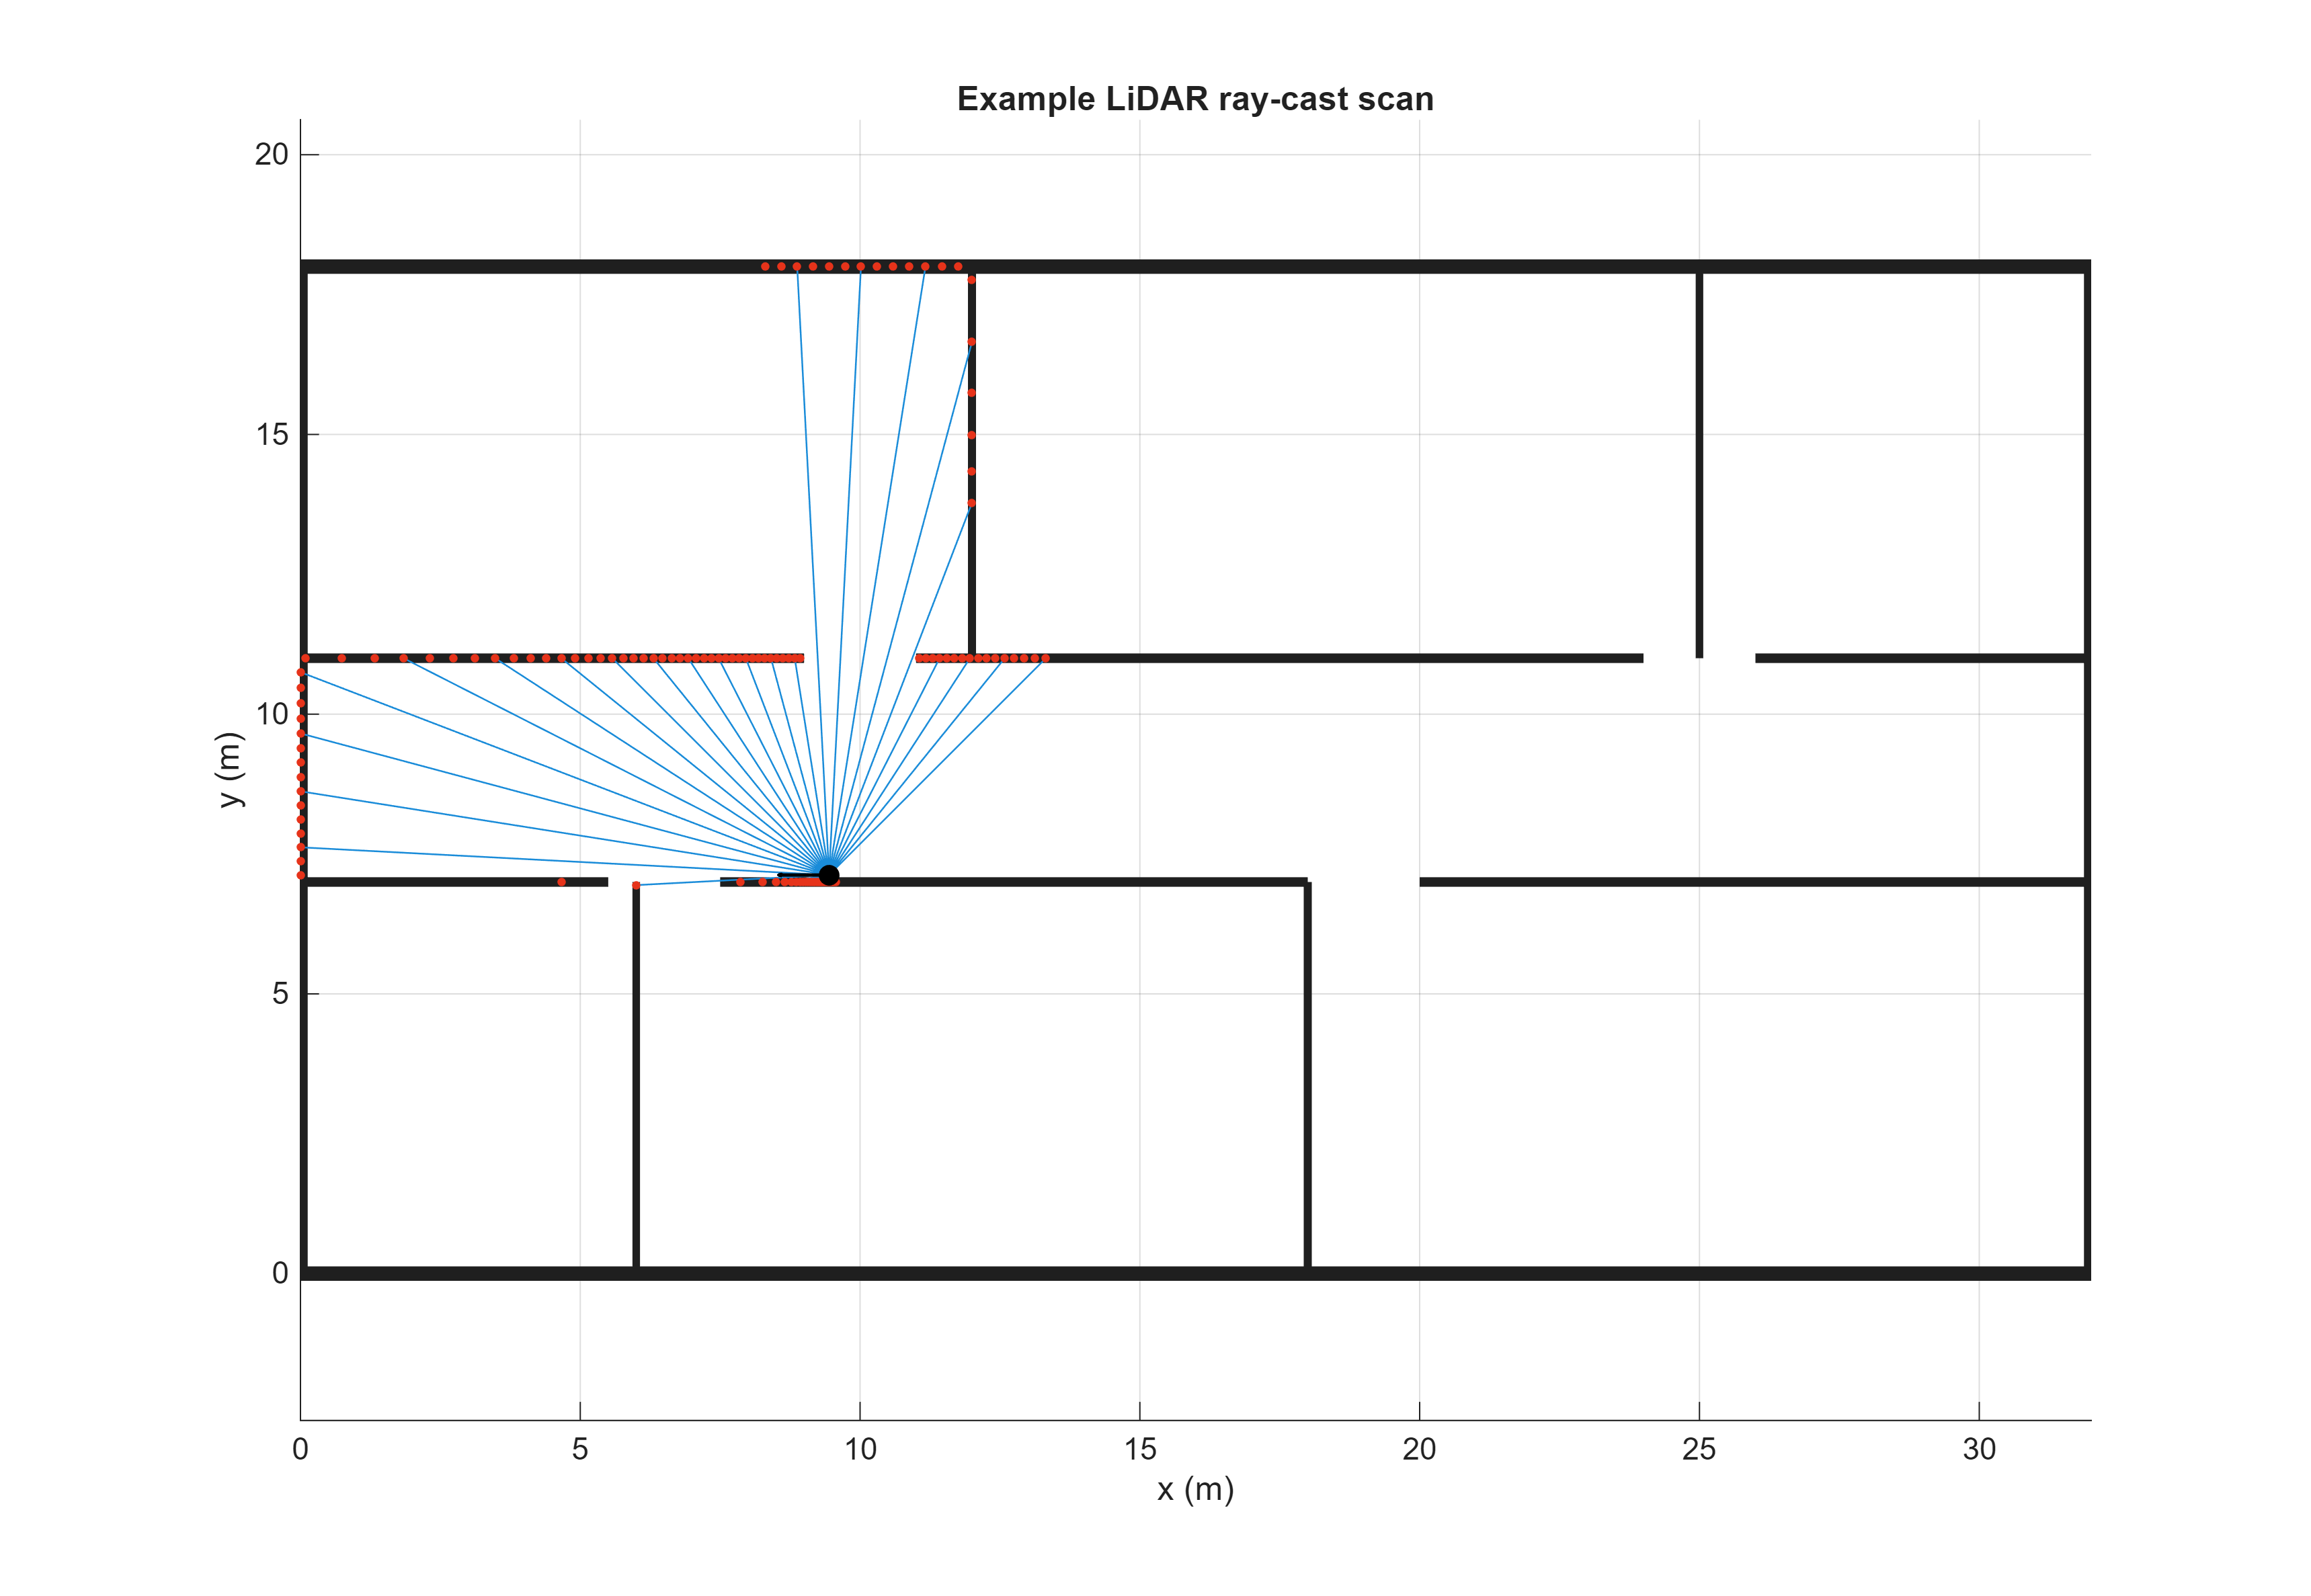
\includegraphics[width=0.30\textwidth]{scenario_001_fig_lidar_scan_example.png} &
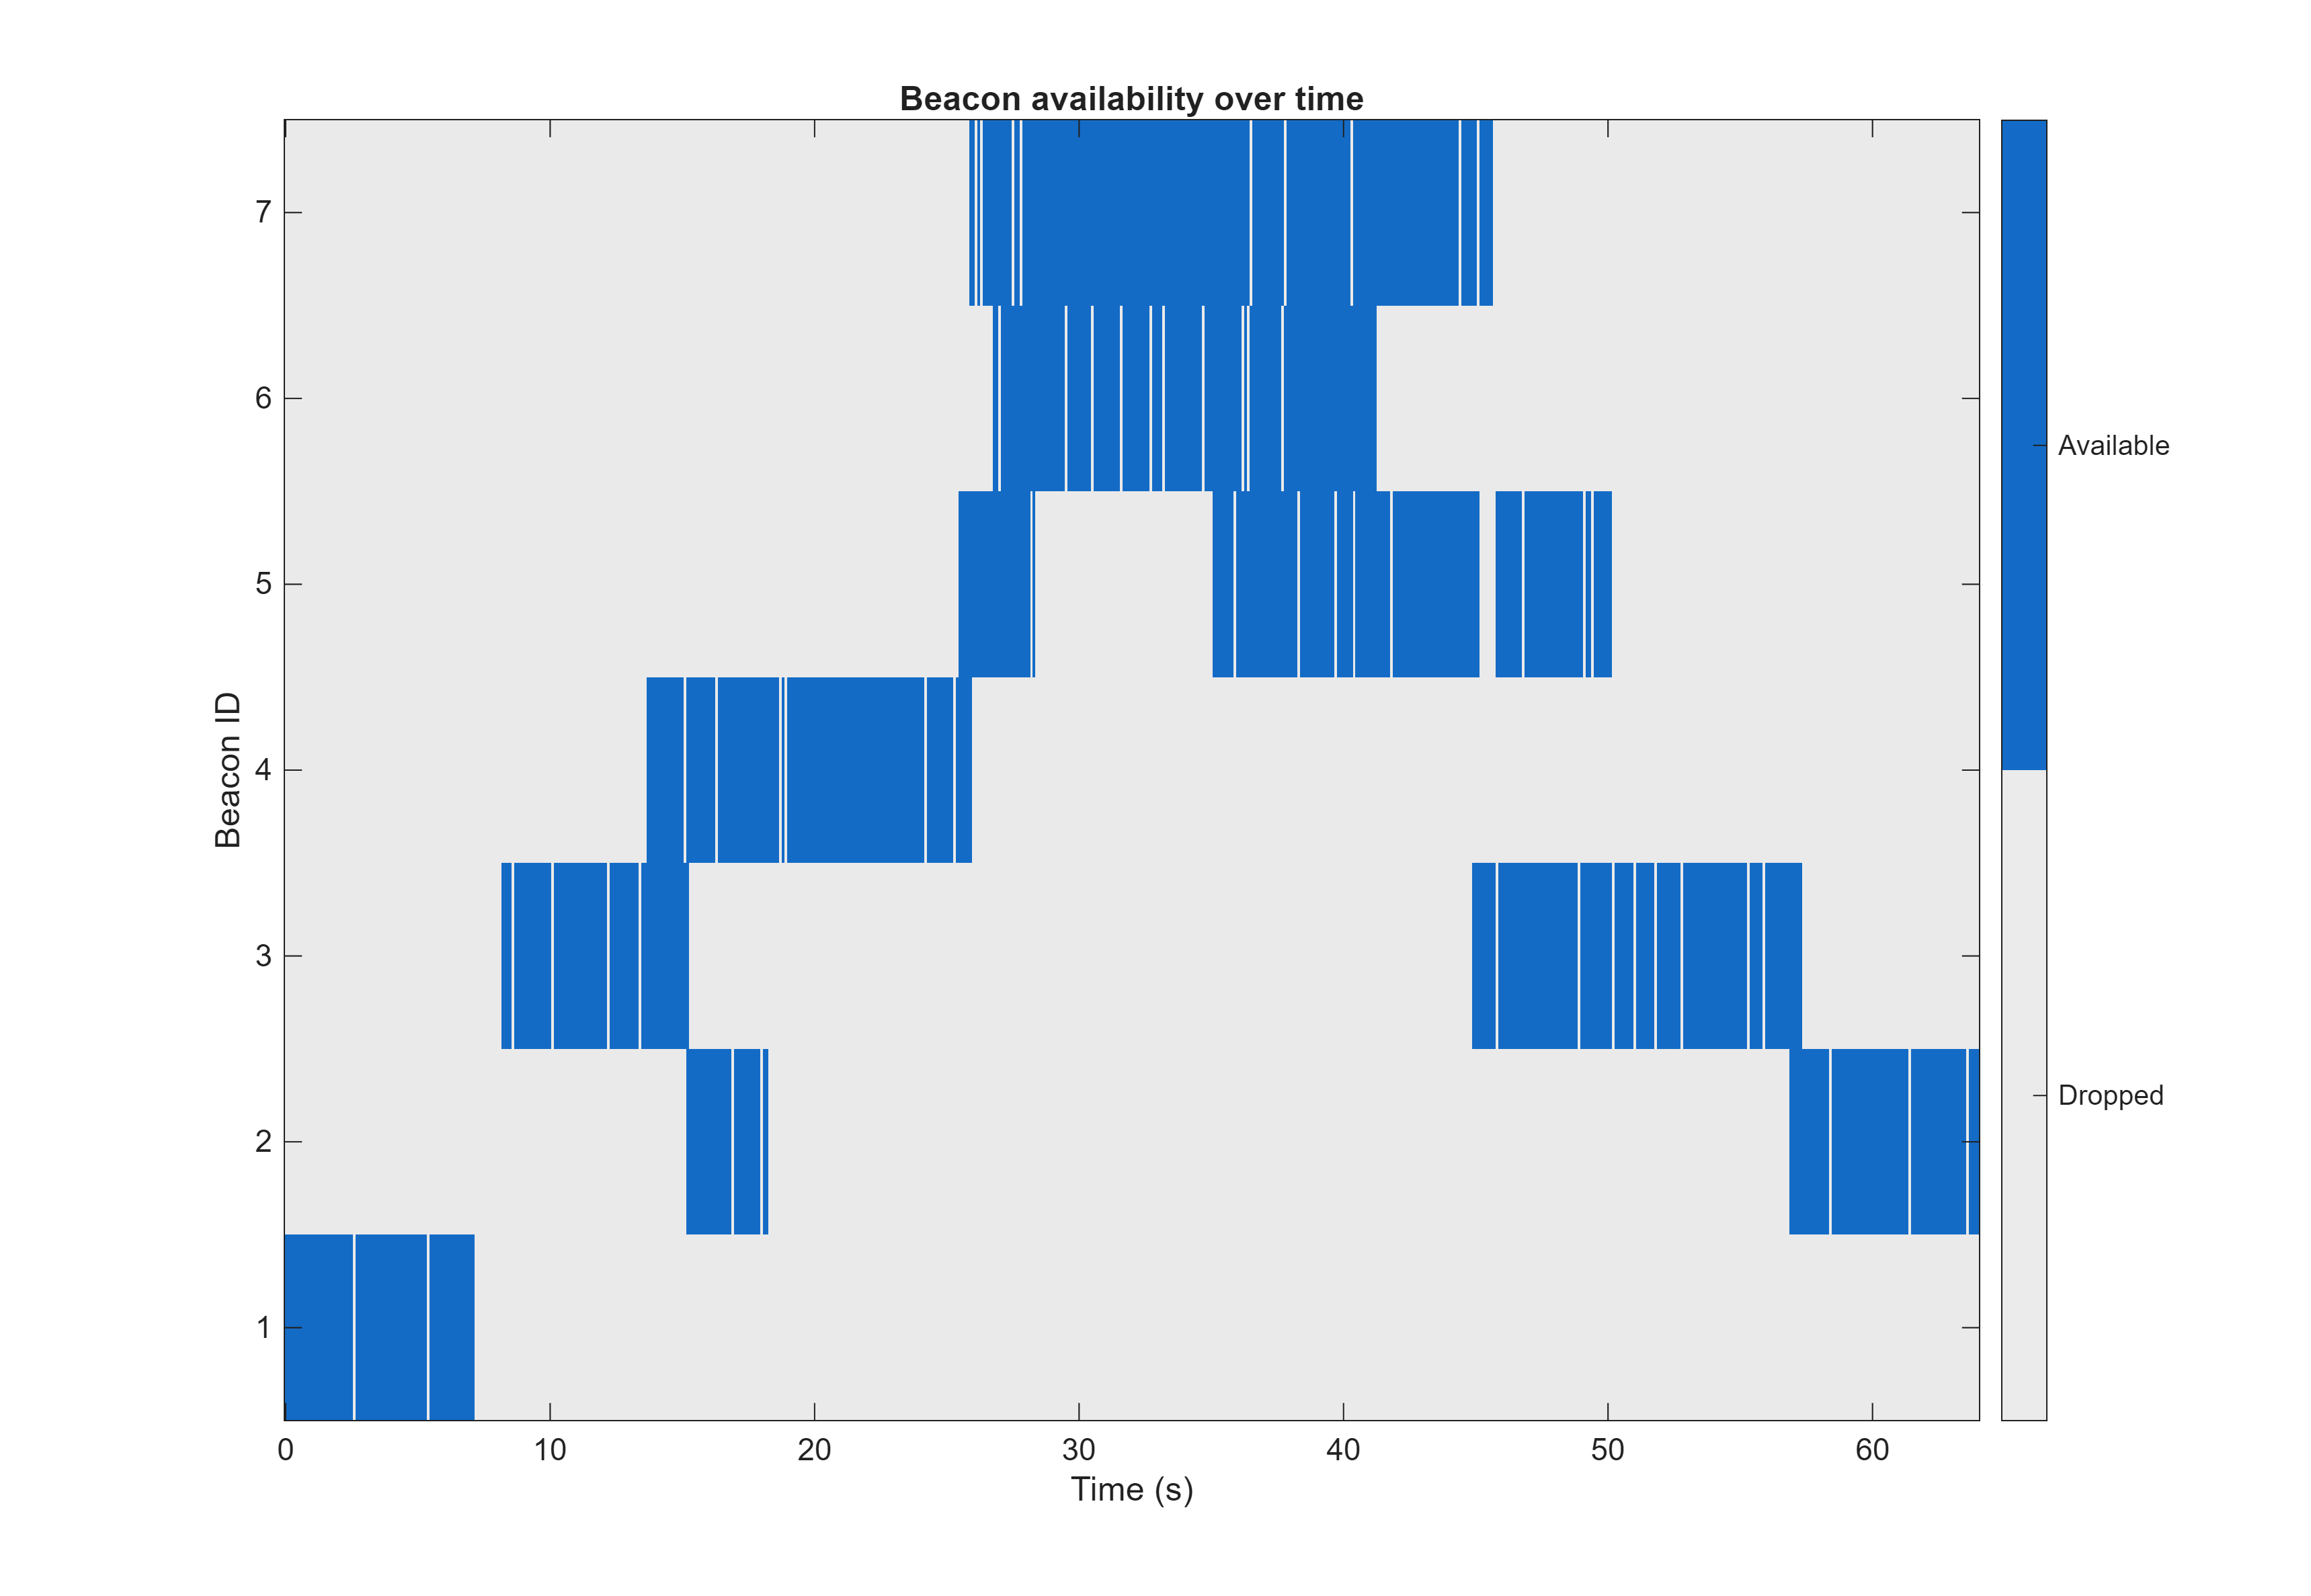
\includegraphics[width=0.30\textwidth]{scenario_002_fig_beacon_availability.png} &
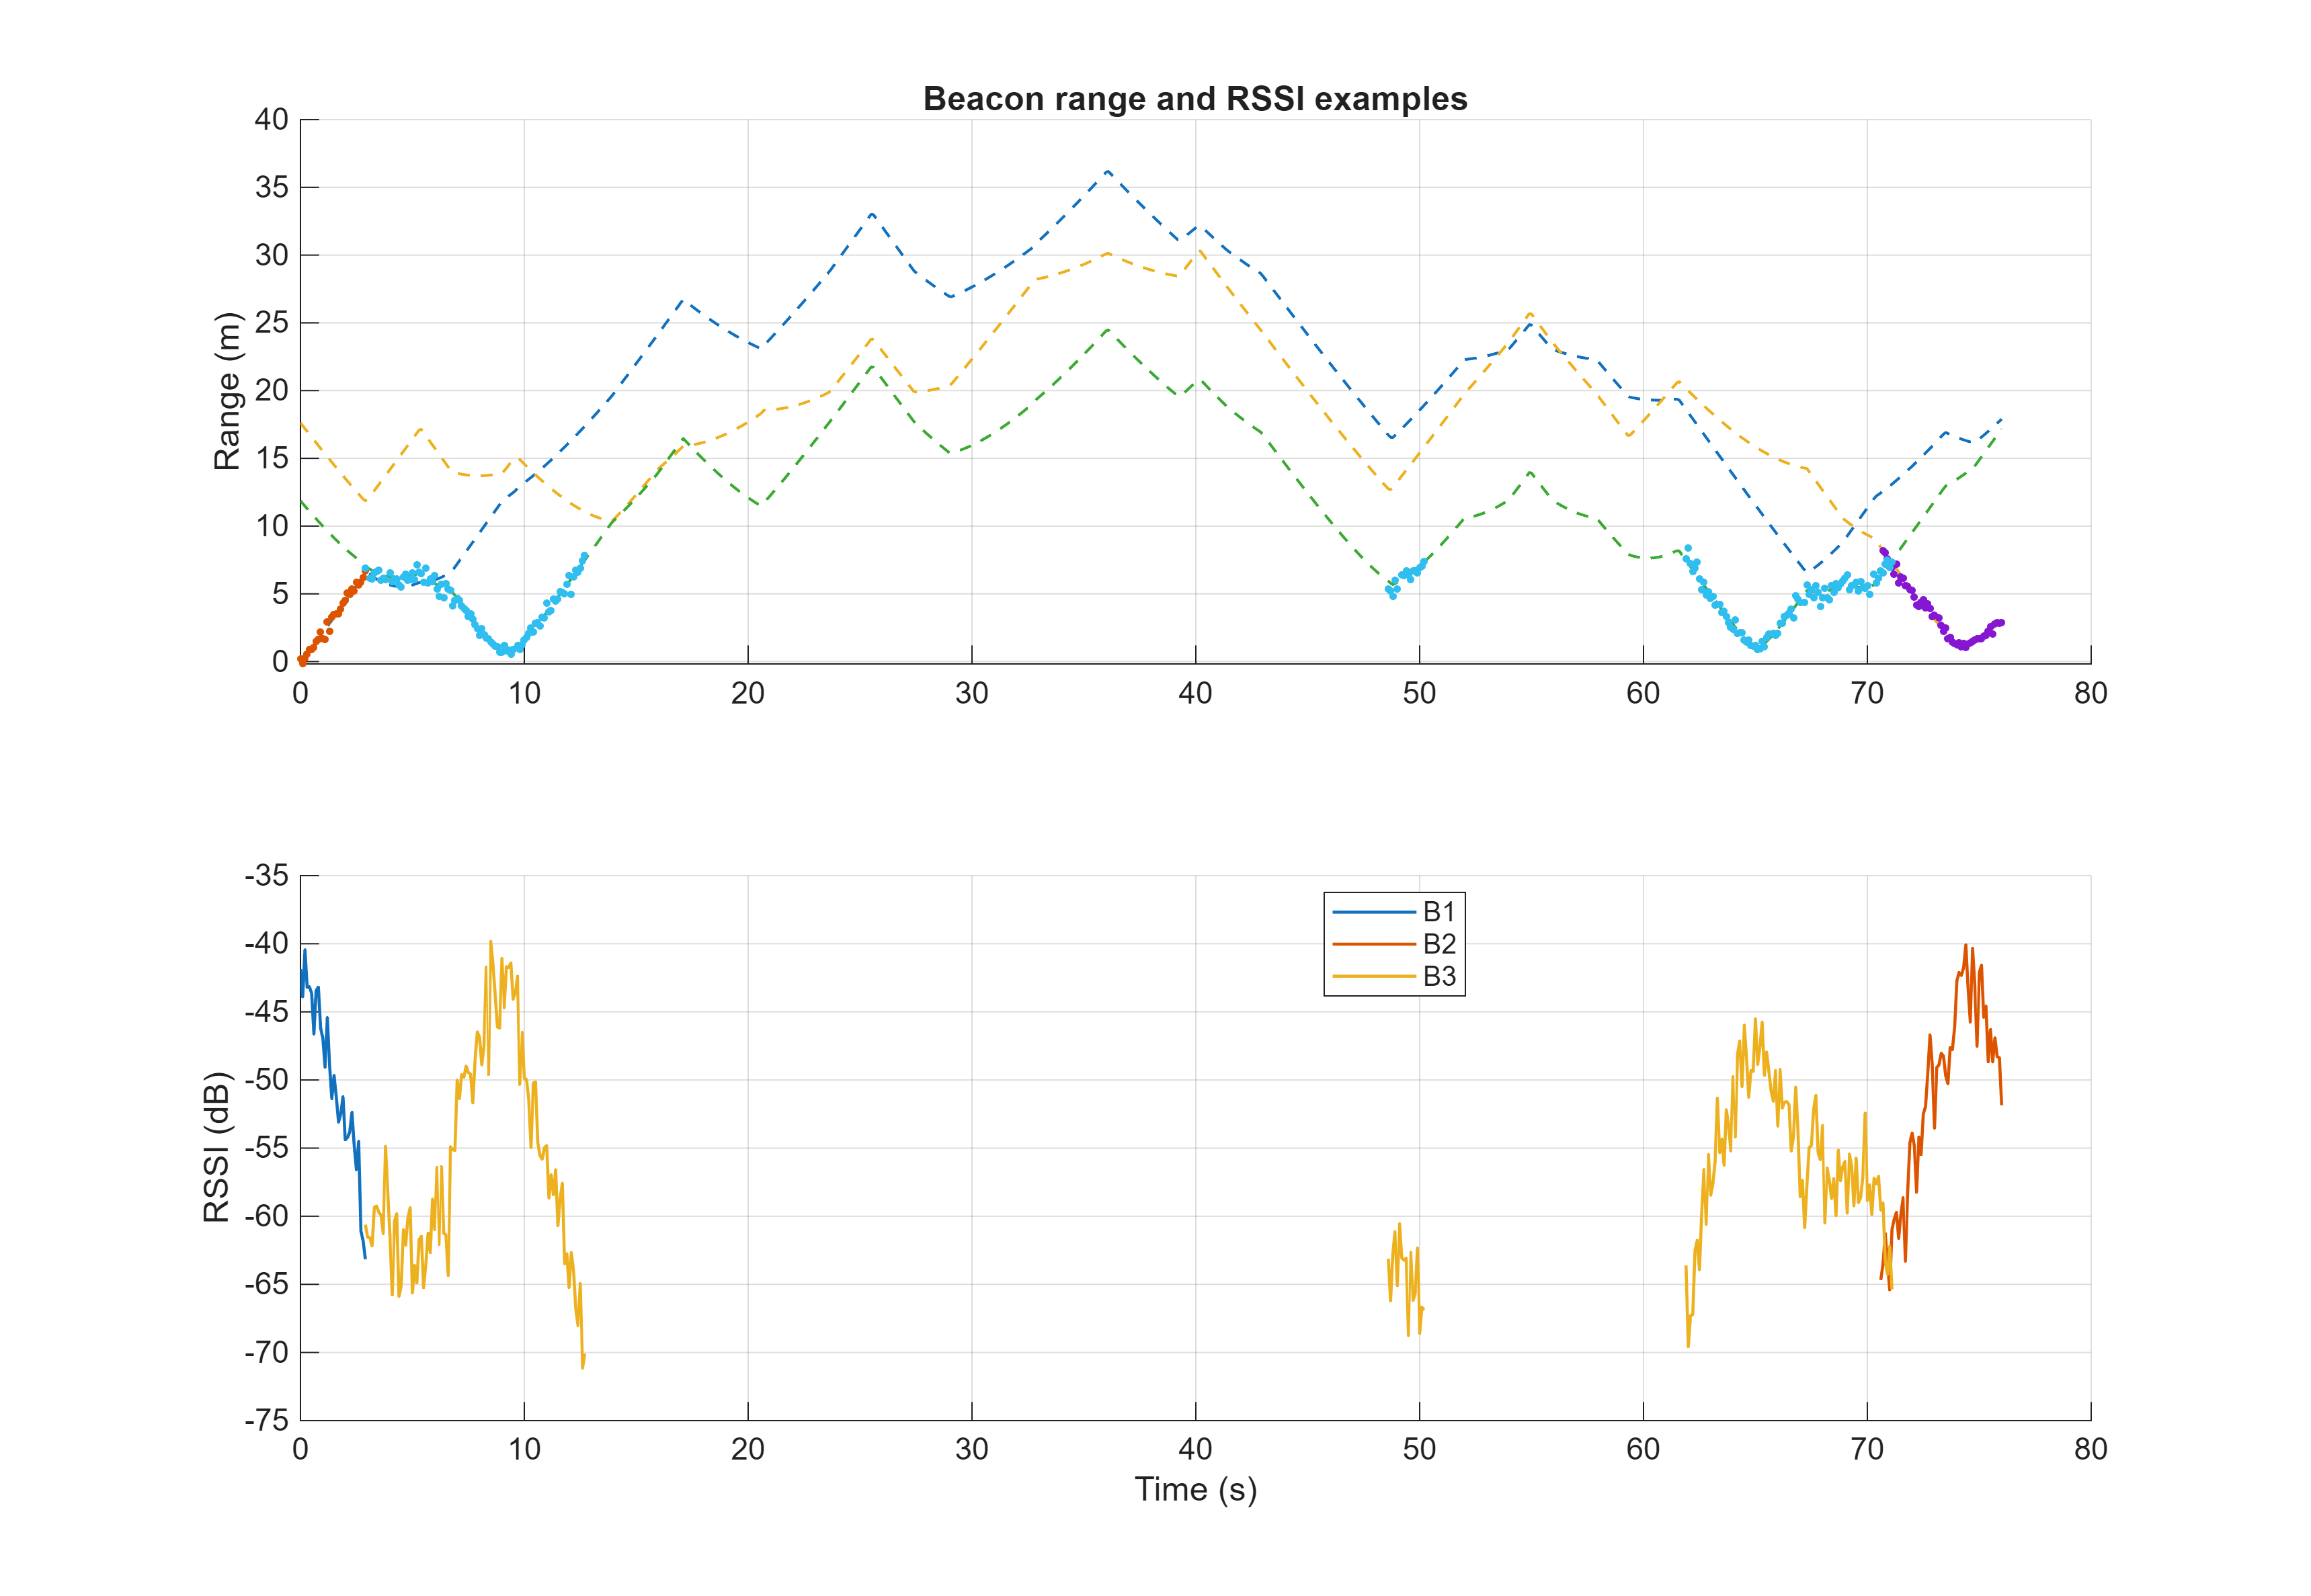
\includegraphics[width=0.30\textwidth]{scenario_003_fig_beacon_signal_profile.png}\\
(a) LiDAR scan example & (b) Beacon availability & (c) Beacon signal profile
\end{tabular}
\caption{Representative sensor behavior from the saved figures. Panel (a) shows ray-cast LiDAR returns, panel (b) shows beacon dropout and availability over time, and panel (c) shows range/RSSI behavior for selected beacons.}
\label{fig:sensor_behavior}
\end{figure*}

\begin{figure*}
\centering
\begin{tabular}{cc}
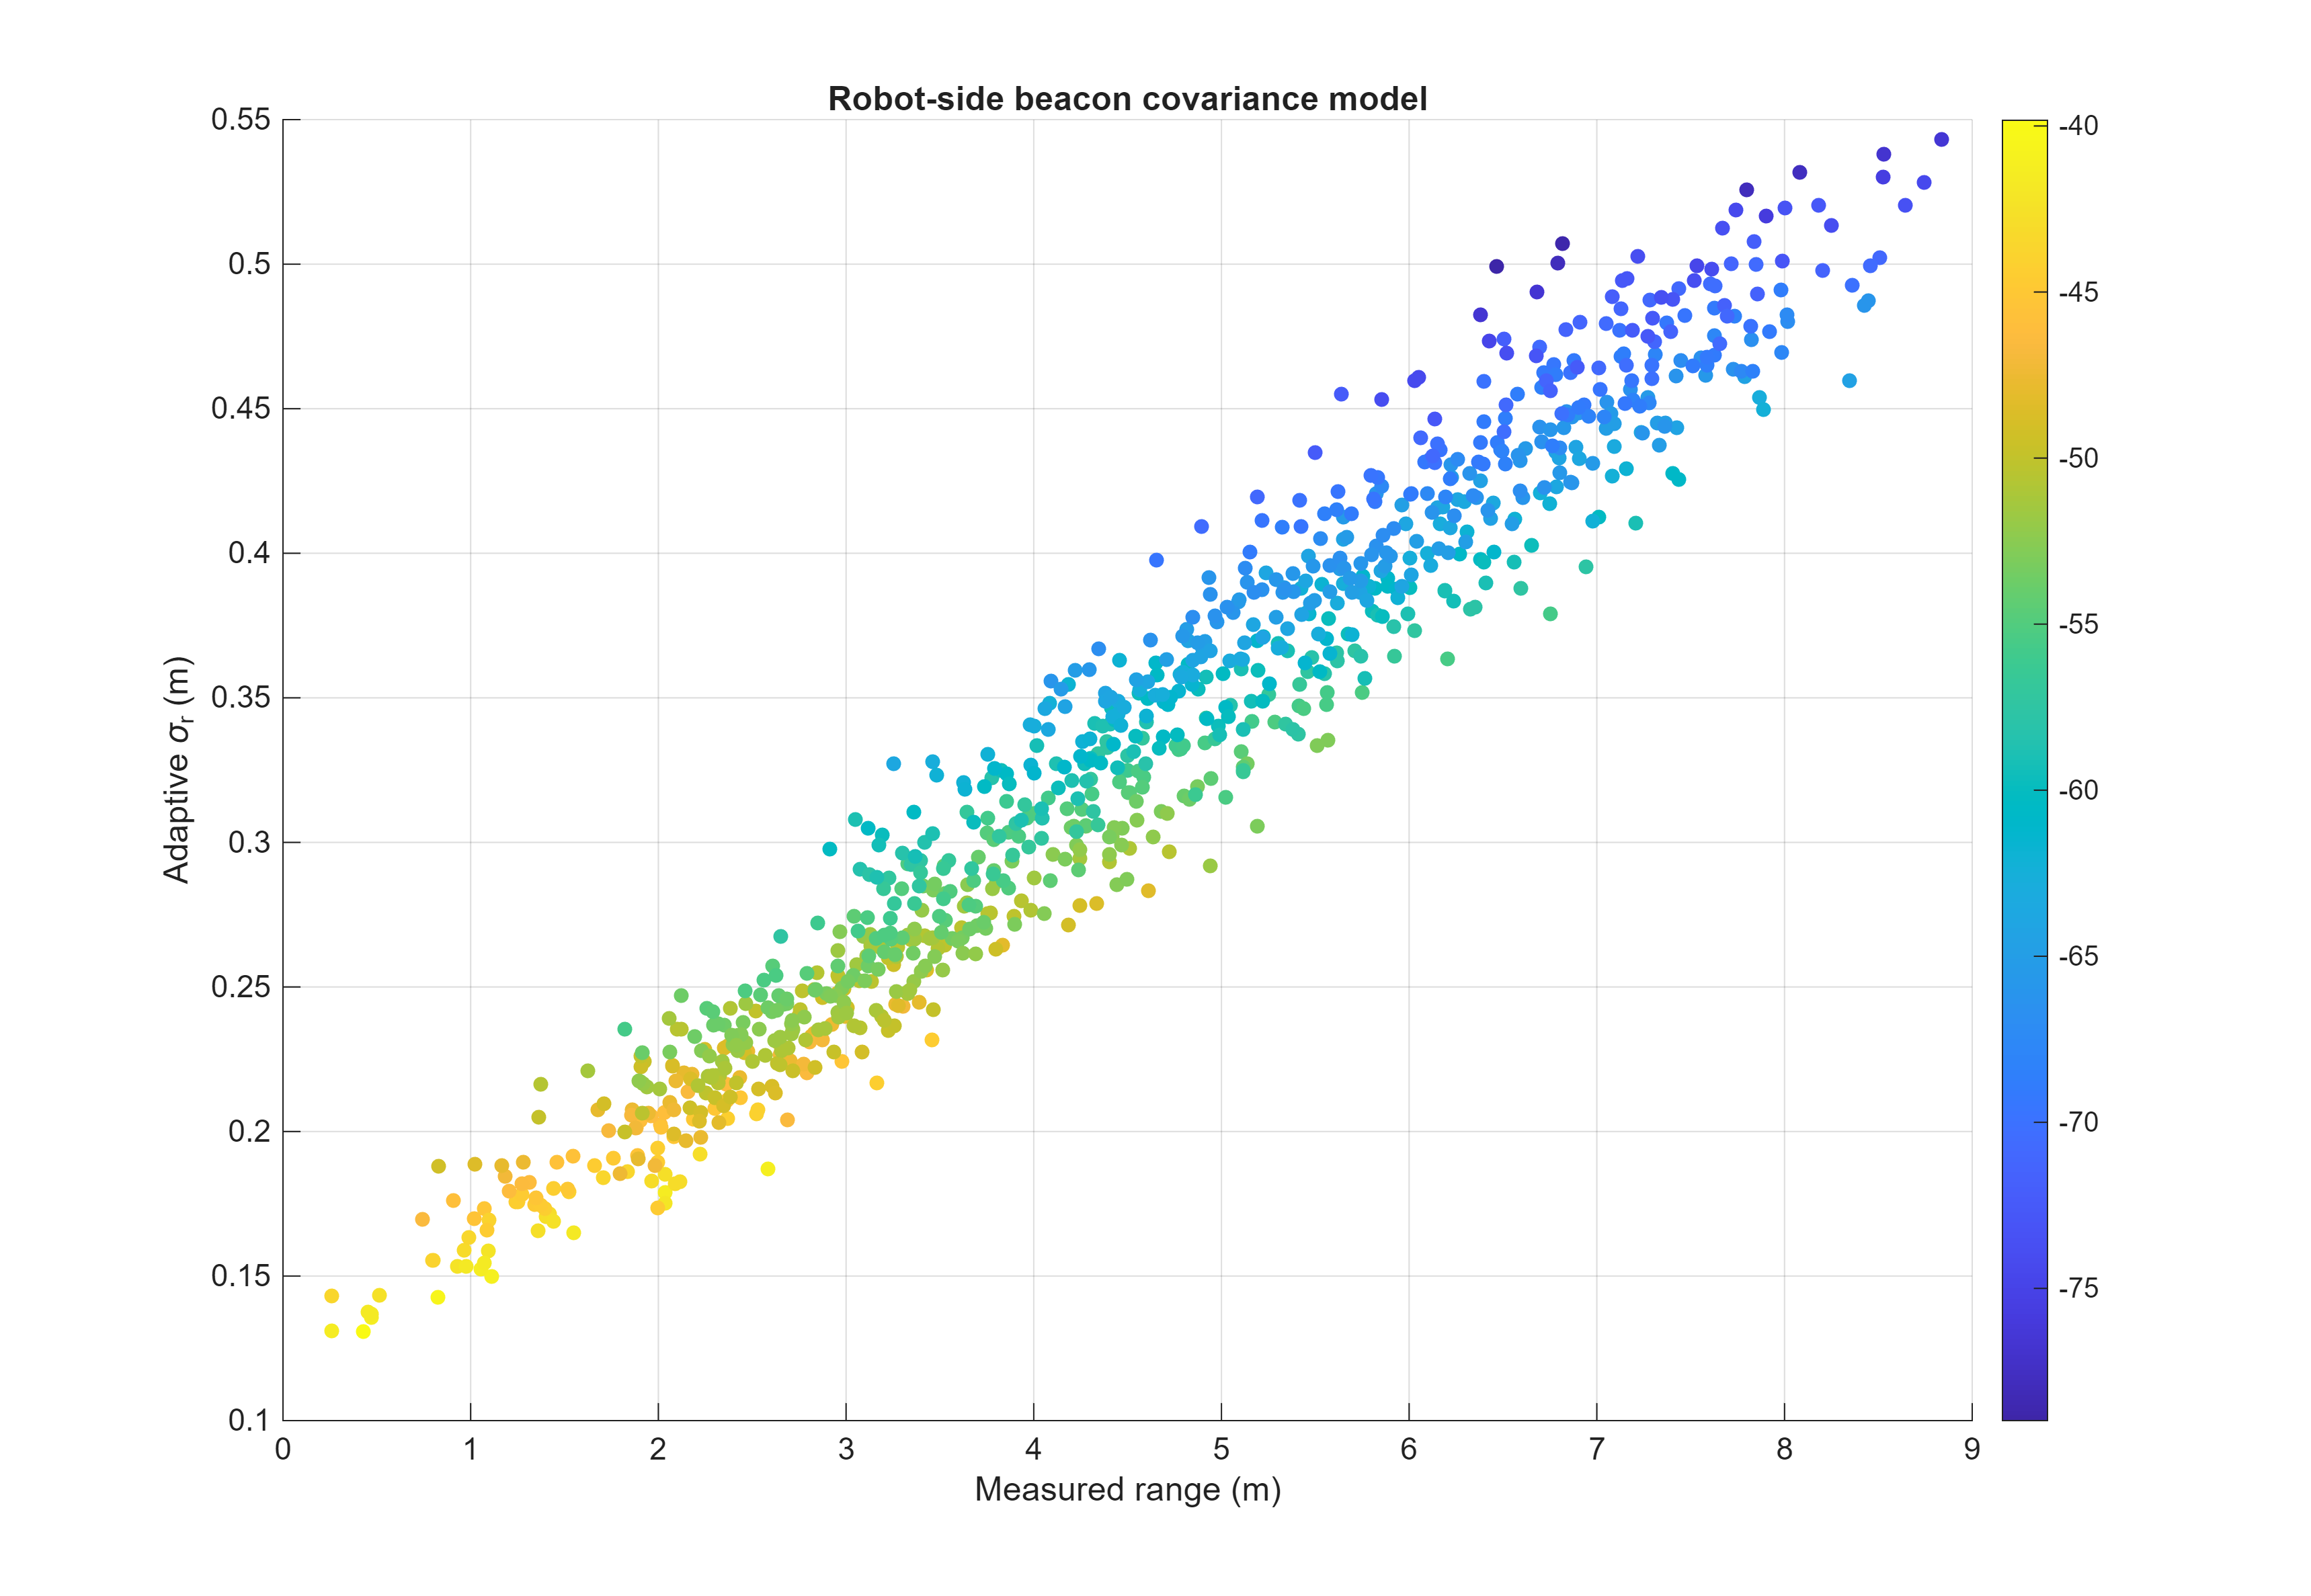
\includegraphics[width=0.46\textwidth]{scenario_002_fig_beacon_noise_model.png} &
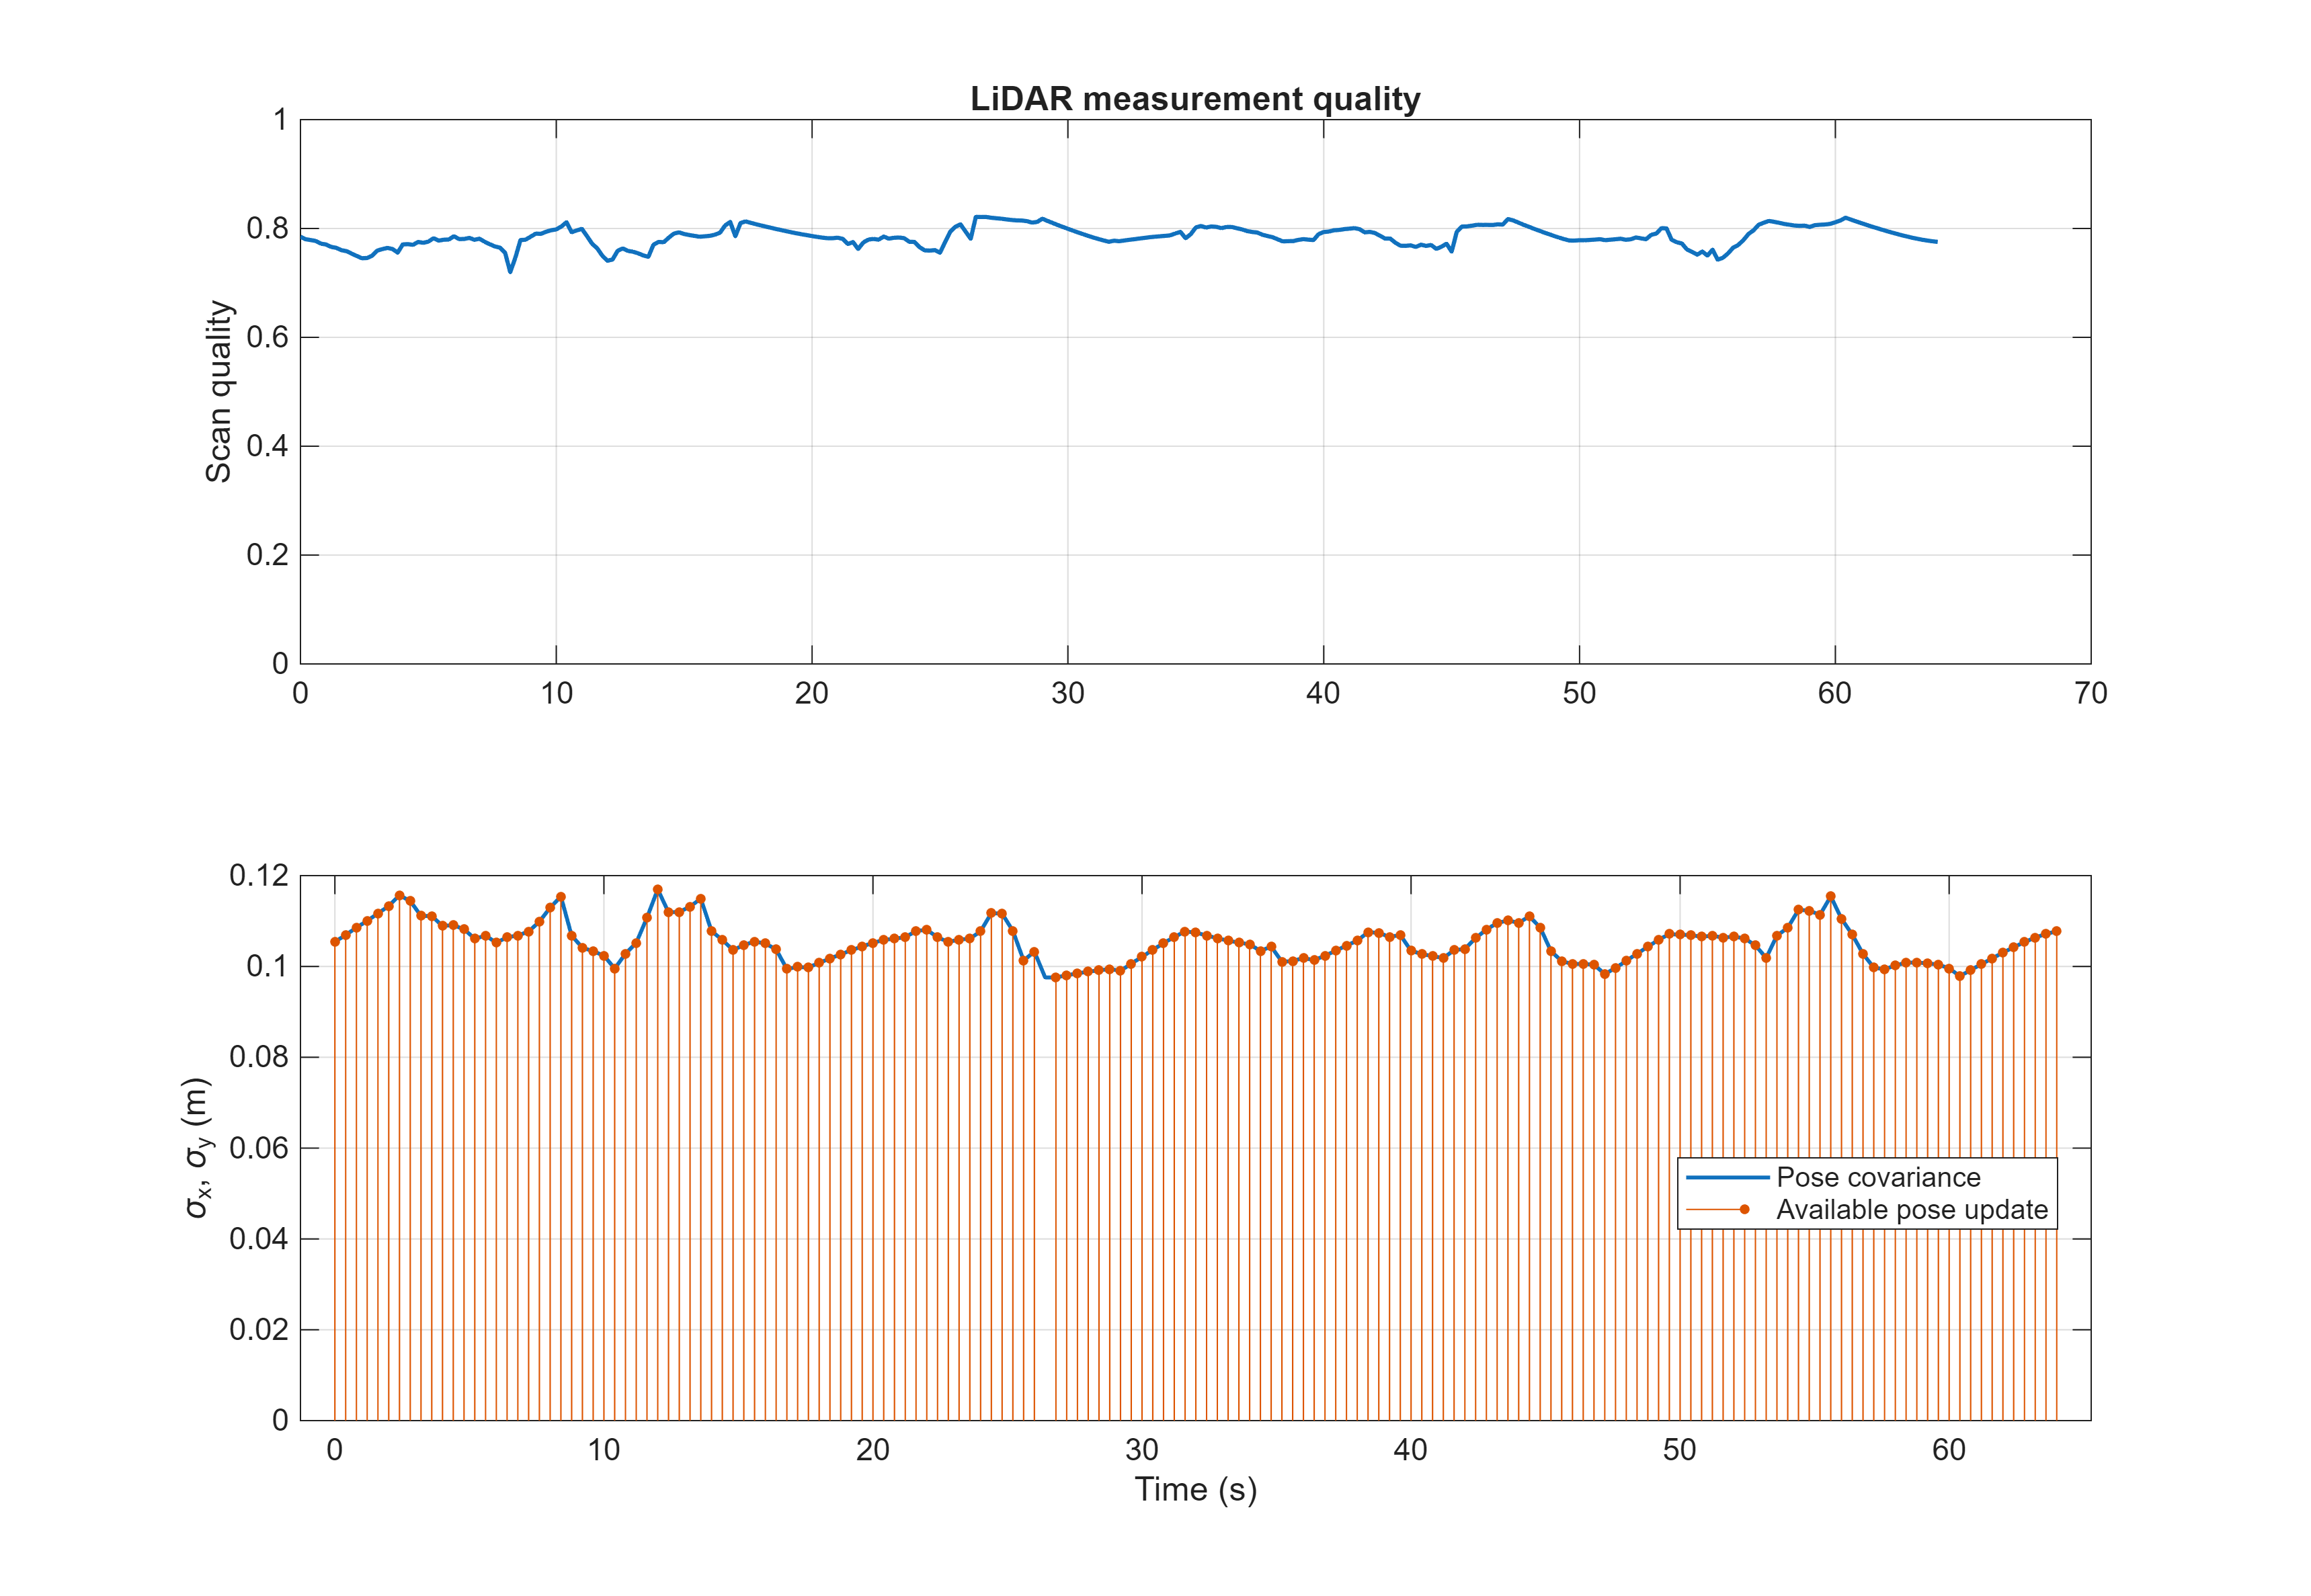
\includegraphics[width=0.46\textwidth]{scenario_002_fig_lidar_quality.png}\\
(a) Beacon covariance model & (b) LiDAR scan quality
\end{tabular}
\caption{Representative measurement-noise behavior. The beacon filter covariance is a function of measured range and RSSI; the LiDAR pose covariance is a function of scan quality.}
\label{fig:noise_behavior}
\end{figure*}

\section{Experiments}

Each filter case is run on the same saved scenario data, so differences between cases are due to estimator configuration rather than regenerated measurements. The cases are:
\begin{enumerate}
    \item Dead reckoning: prediction only.
    \item Beacon fixed covariance: prediction plus available beacon ranges with \(0.55~\mathrm{m}\) standard deviation.
    \item Beacon adaptive covariance: prediction plus available beacon ranges using Eq.~(\ref{eq:adaptive_sigma}).
    \item LiDAR only: prediction plus synthetic LiDAR pose updates.
    \item LiDAR plus adaptive beacons: prediction plus synthetic LiDAR pose updates and adaptive beacon range updates.
\end{enumerate}

\begin{table}
\centering
\caption{Filter case configuration.}
\label{tab:filter_cases}
\begin{tabular}{lccc}
\toprule
Case & Beacon & Adaptive & LiDAR\\
\midrule
Dead reckoning & No & No & No\\
Beacon fixed & Yes & No & No\\
Beacon adaptive & Yes & Yes & No\\
LiDAR only & No & No & Yes\\
LiDAR + beacon & Yes & Yes & Yes\\
\bottomrule
\end{tabular}
\end{table}

\subsection{Metrics}

Metrics are computed against the saved ground truth by \texttt{compute\_filter\_metrics.m}. The position, heading, and velocity RMSE definitions are
\begin{align}
    \mathrm{RMSE}_p &=
    \sqrt{\frac{1}{N}\sum_{k=1}^{N}\norm{p_k-\hat{p}_k}^{2}},\\
    \mathrm{RMSE}_{\theta} &=
    \sqrt{\frac{1}{N}\sum_{k=1}^{N}
    \wrap(\theta_k-\hat{\theta}_k)^2},\\
    \mathrm{RMSE}_v &=
    \sqrt{\frac{1}{N}\sum_{k=1}^{N}\norm{v_k-\hat{v}_k}^{2}}.
\end{align}
The exported tables also include maximum and median position error, beacon measurement availability percentage, average number of available beacons per beacon update, percentages of zero/one/two/three-or-more beacon availability, LiDAR pose availability percentage, and average LiDAR quality.

\section{Results}

\begin{figure*}
\centering
\begin{tabular}{ccc}
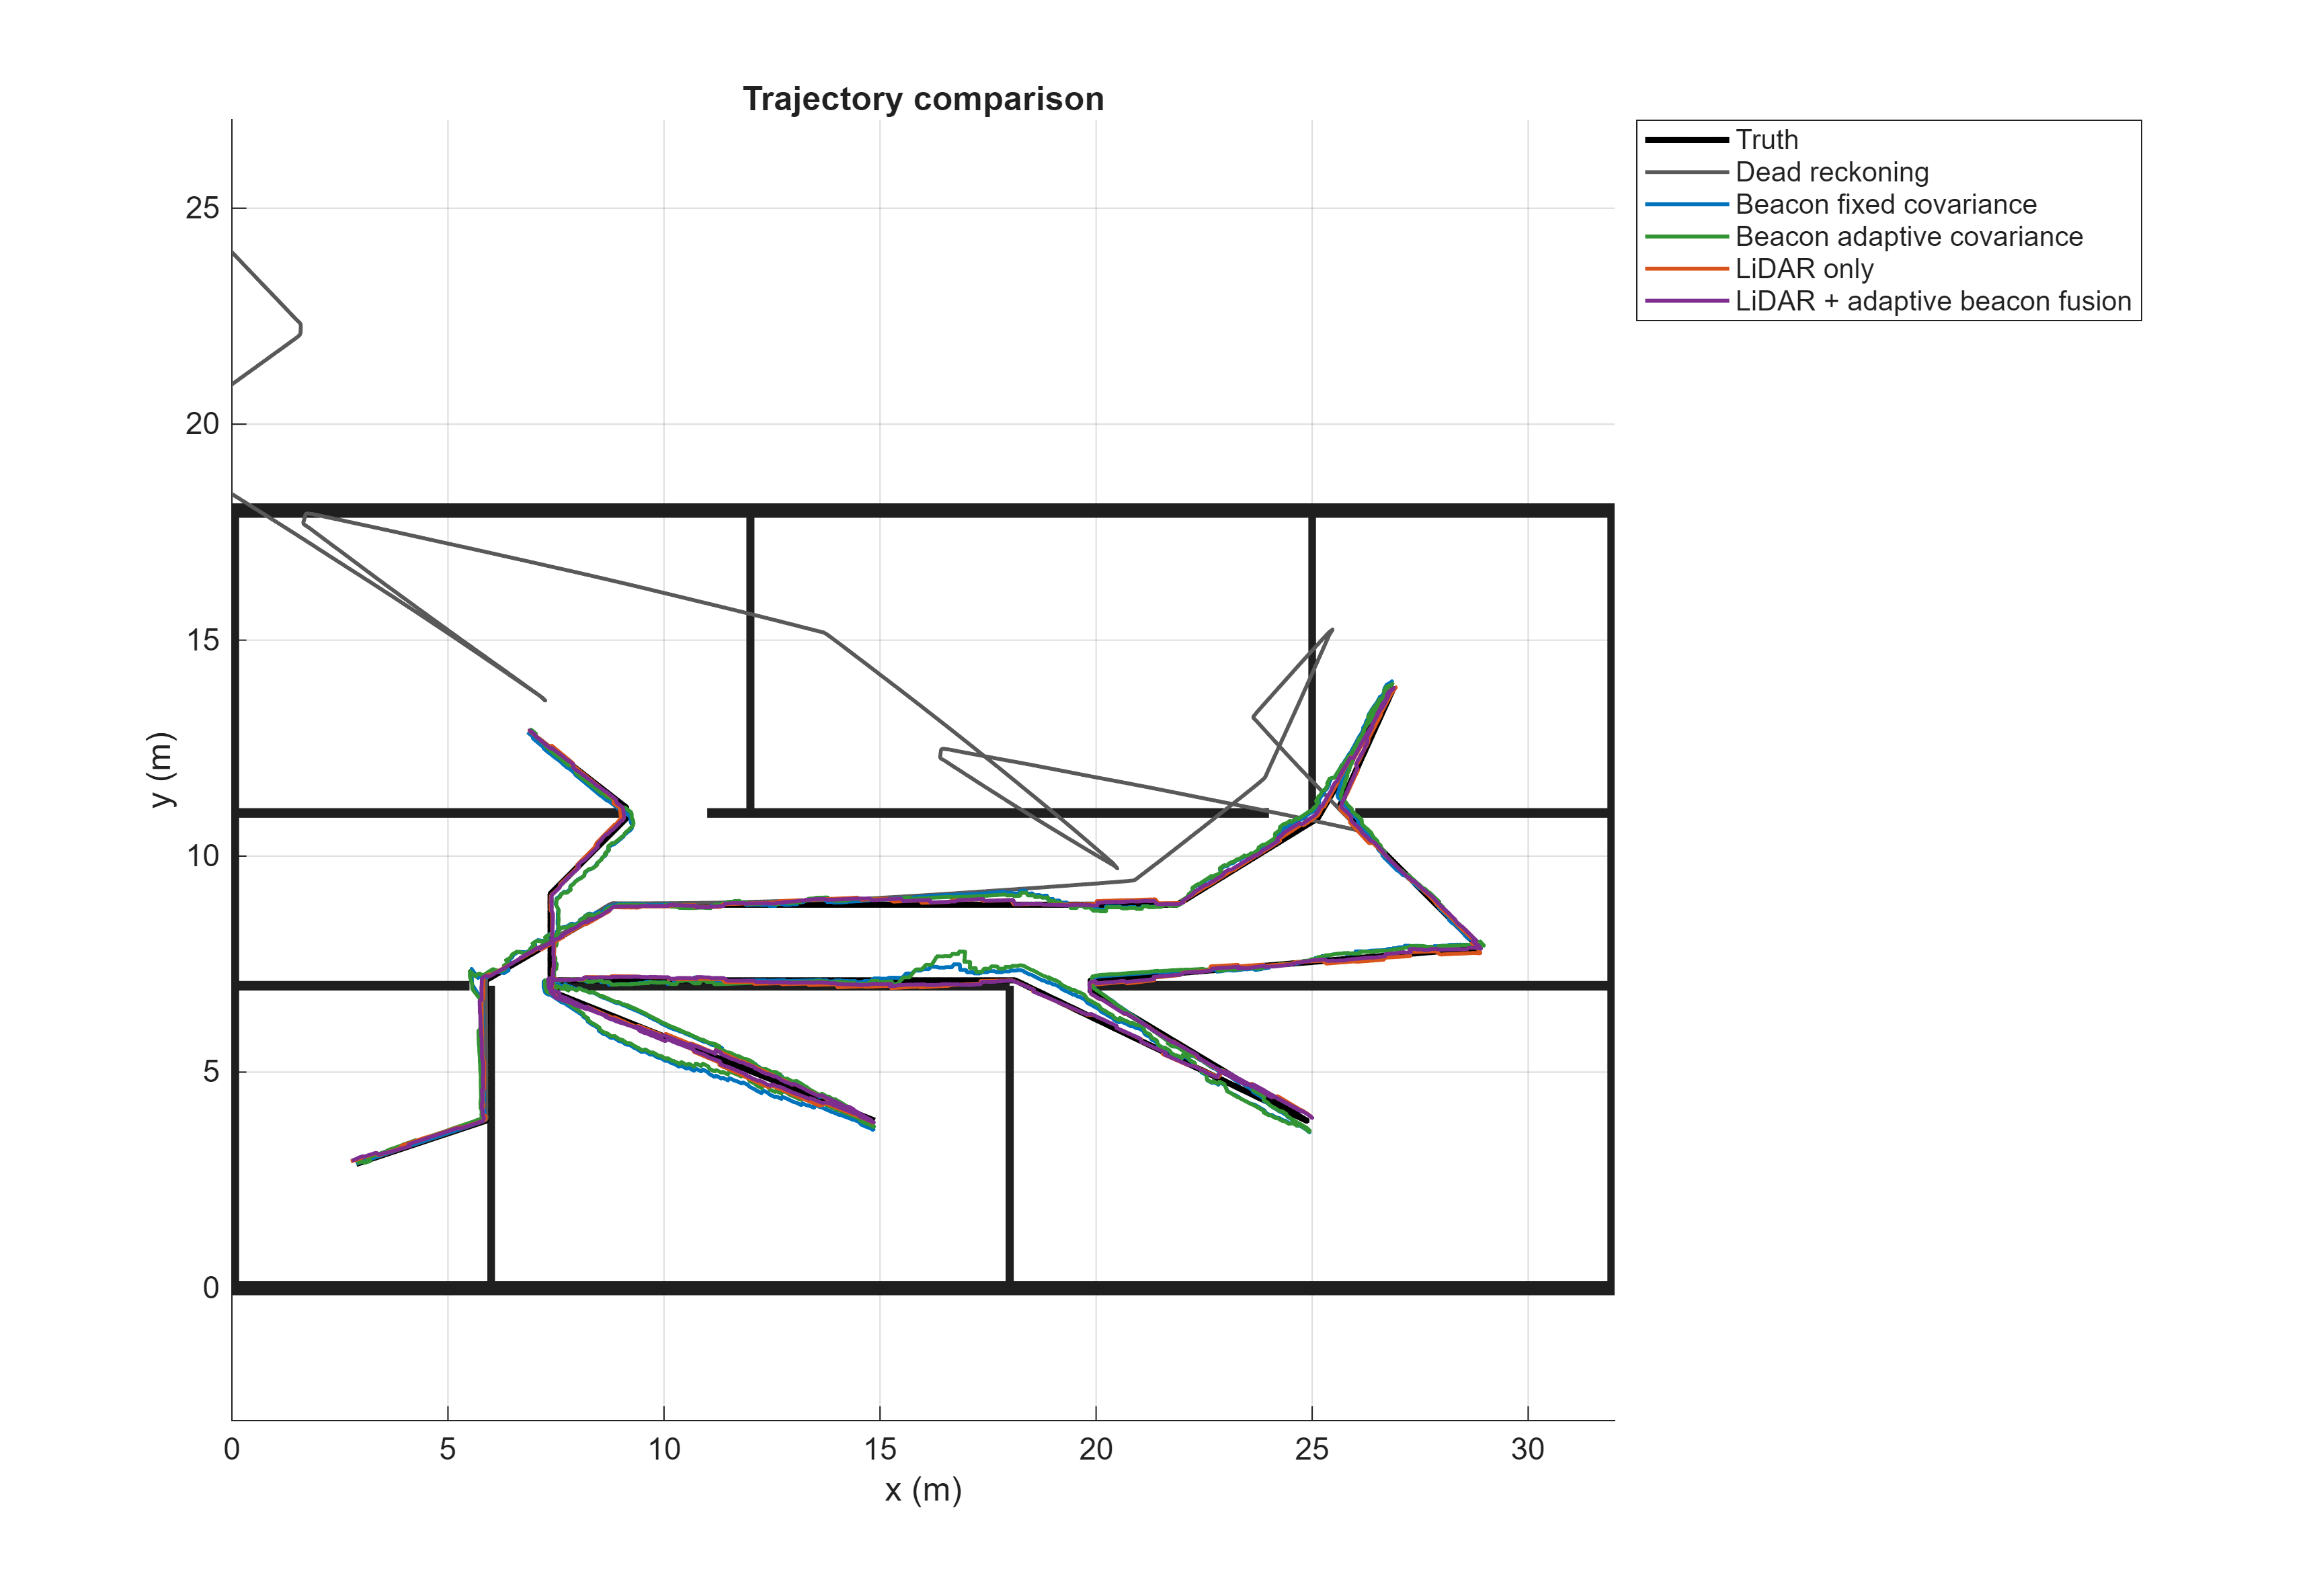
\includegraphics[width=0.30\textwidth]{scenario_001_fig_trajectory_comparison.png} &
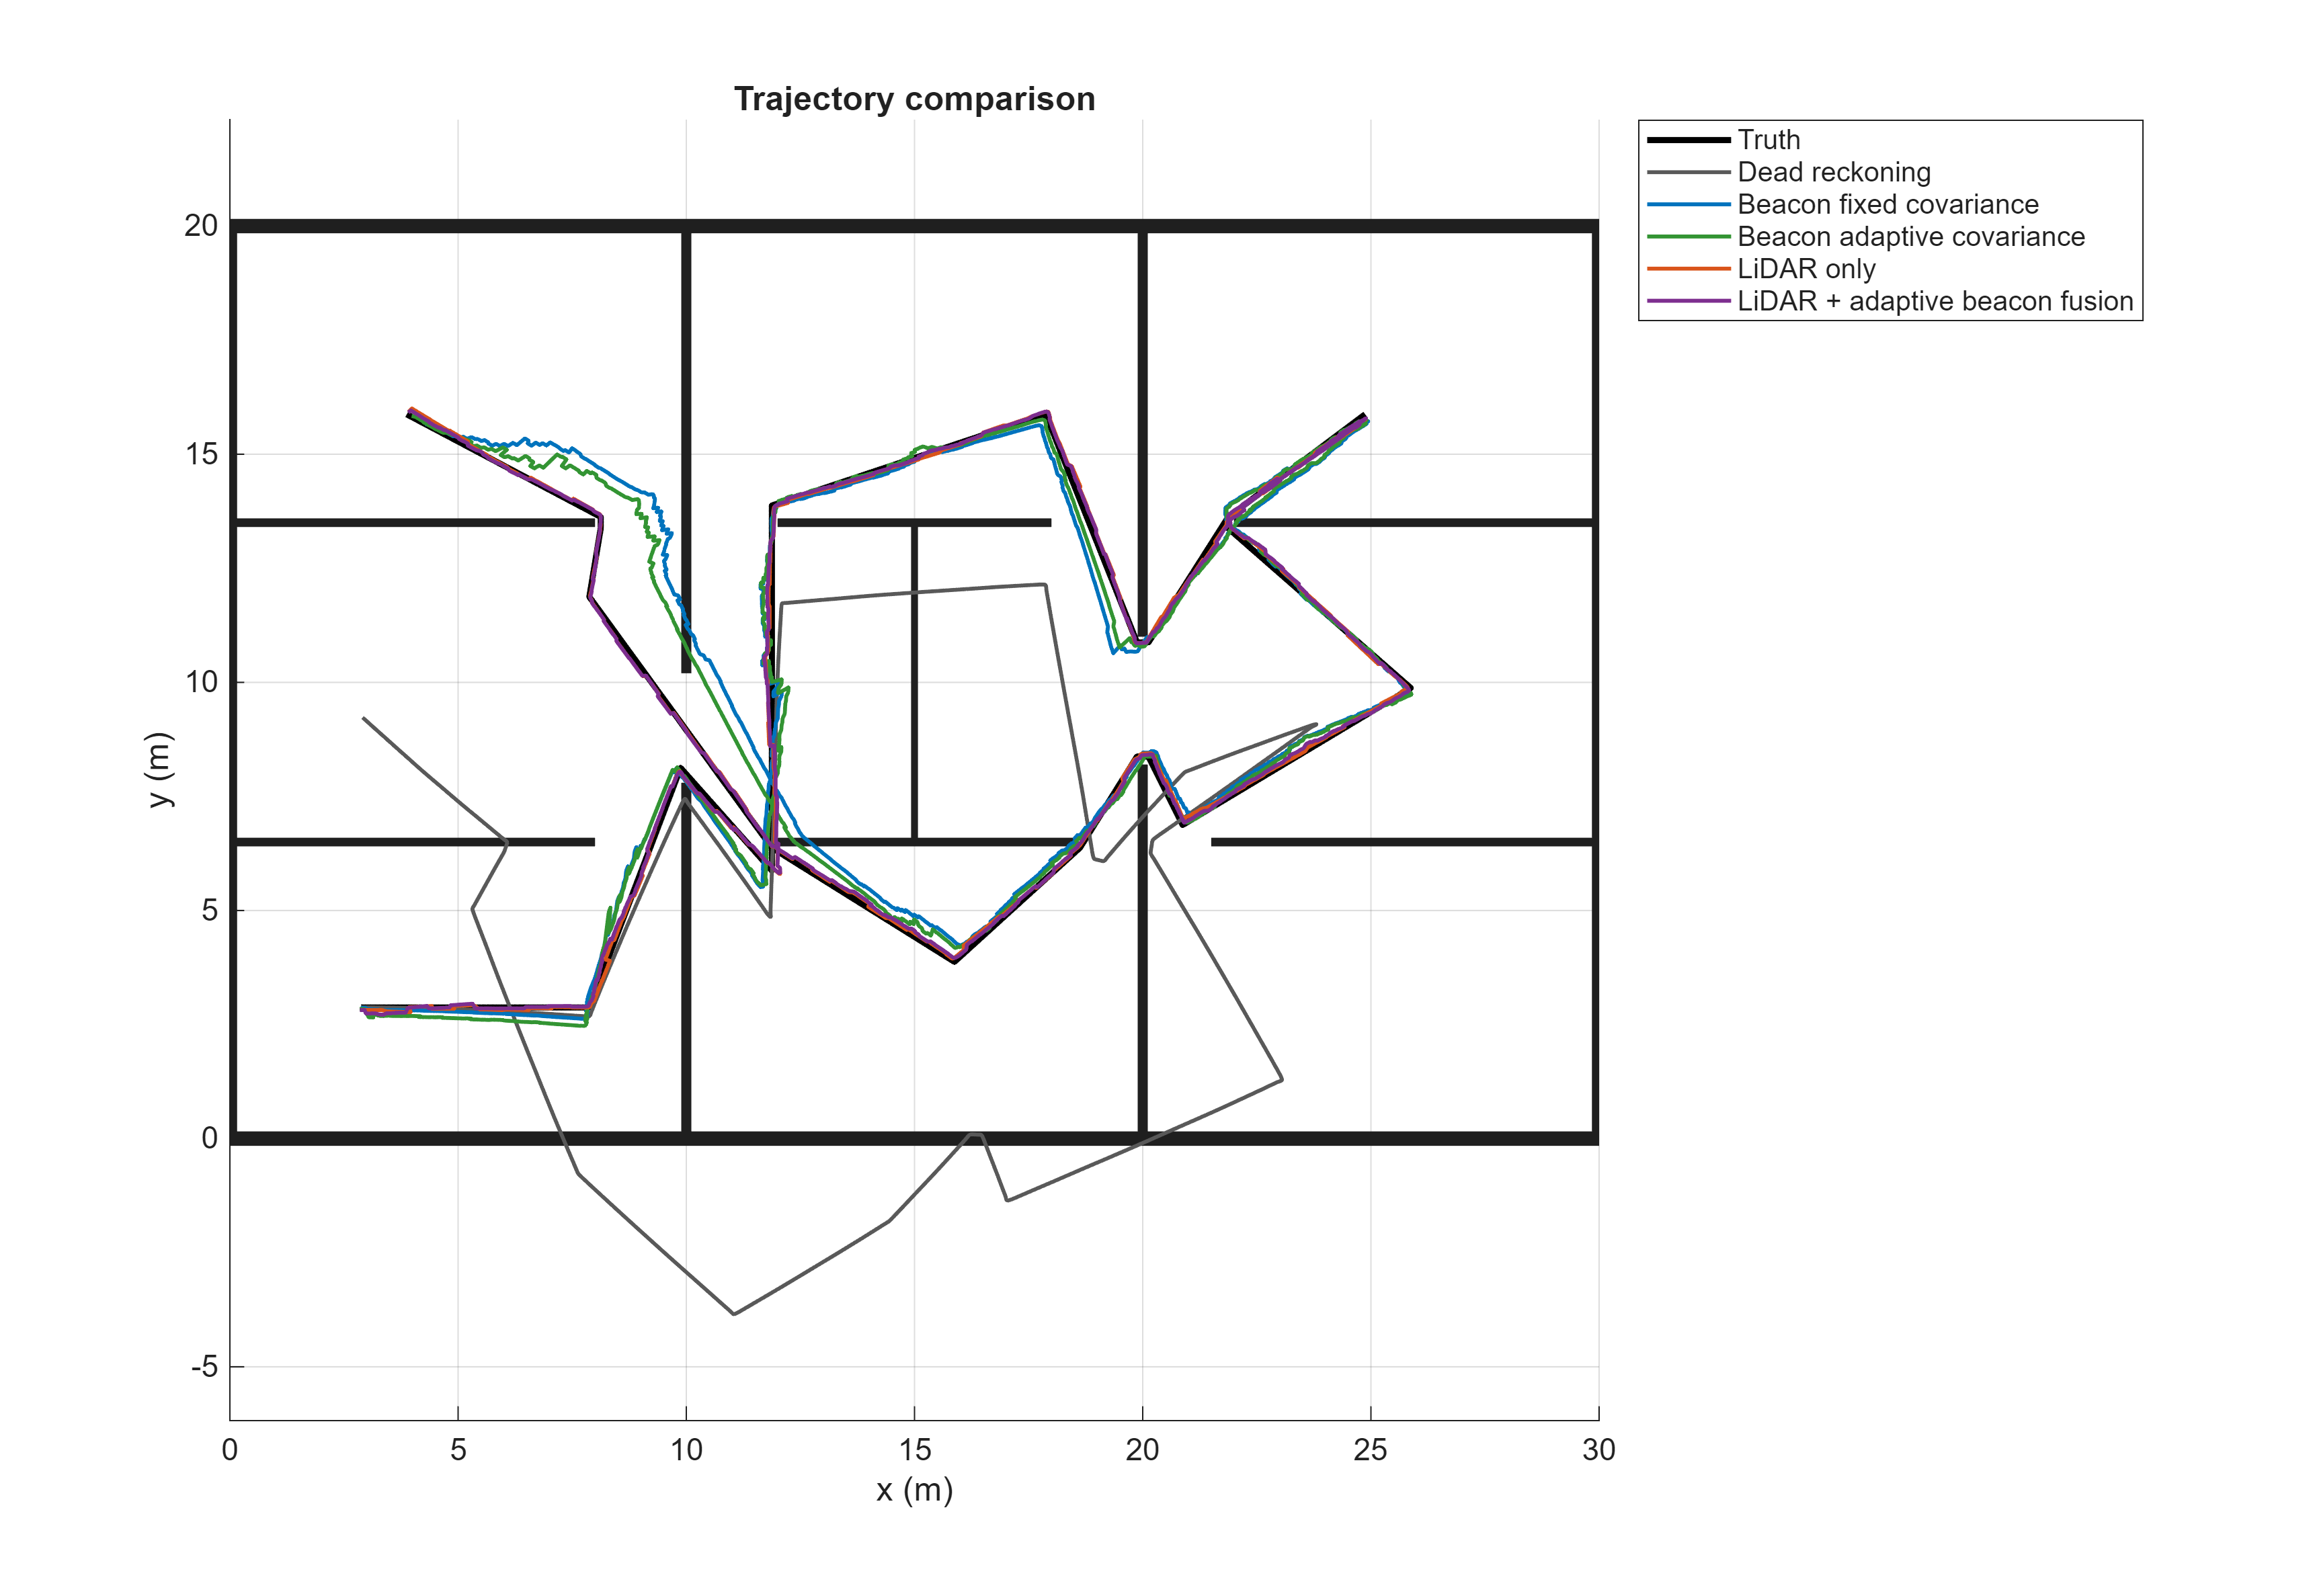
\includegraphics[width=0.30\textwidth]{scenario_002_fig_trajectory_comparison.png} &
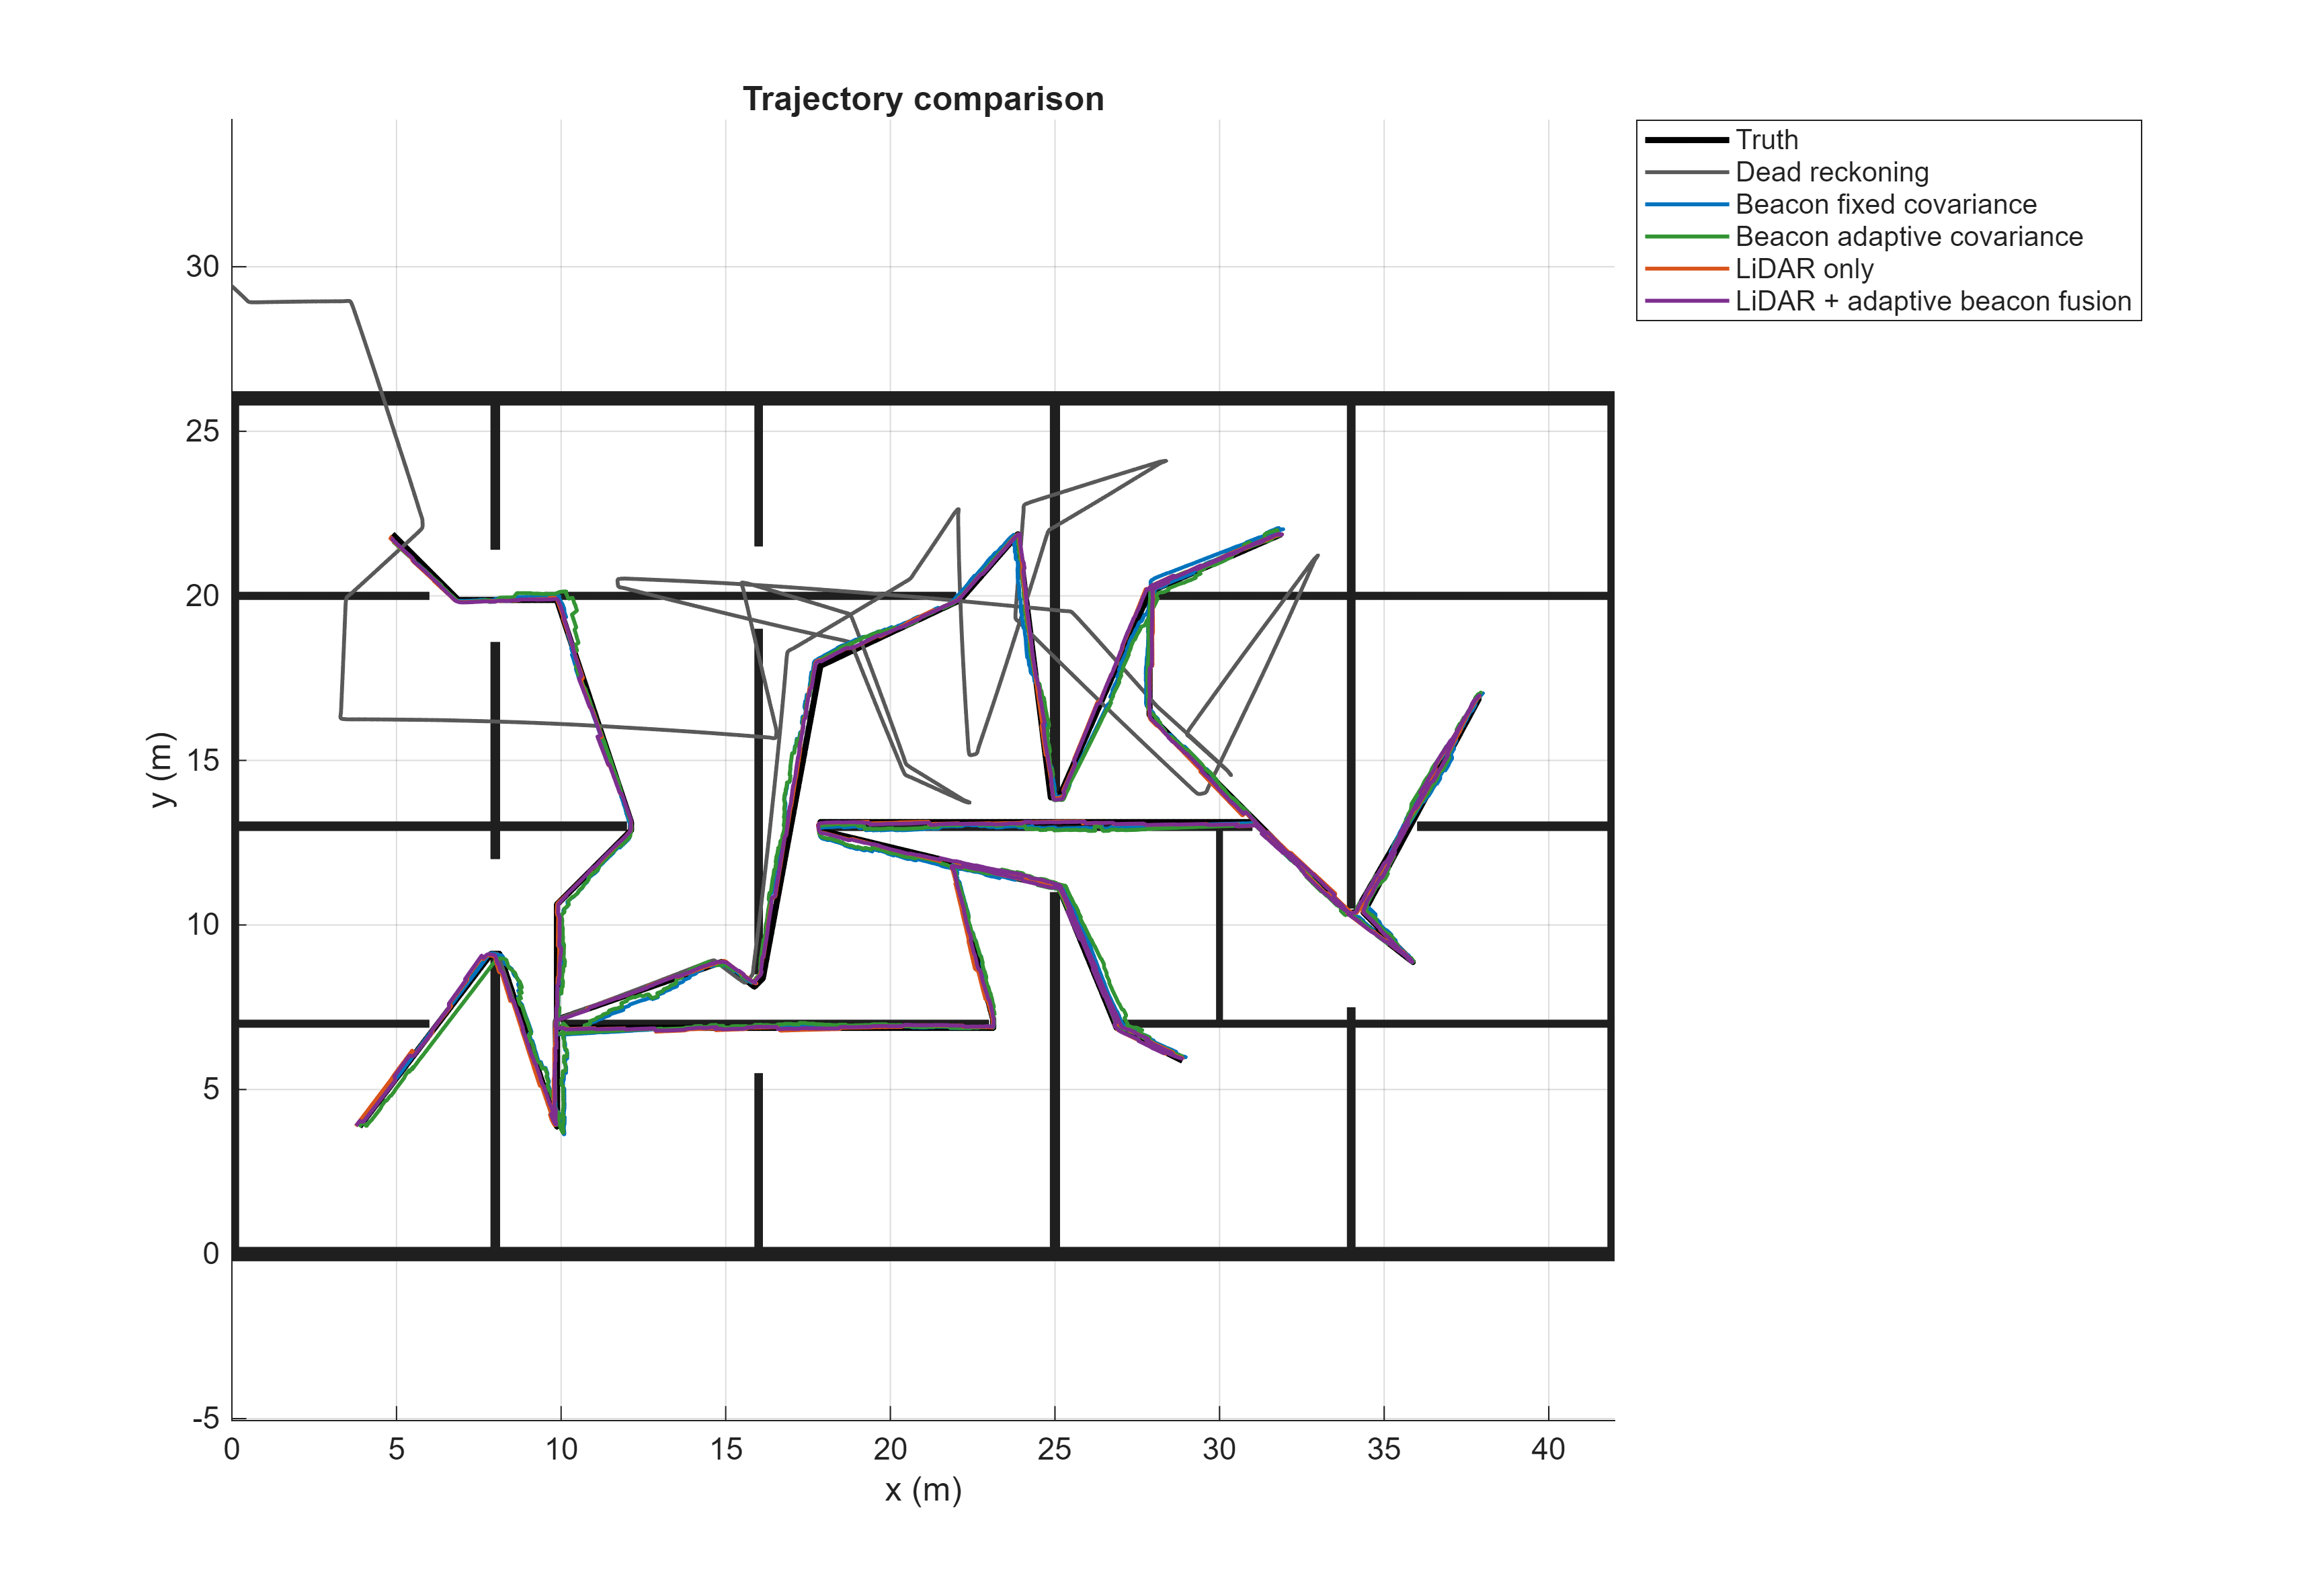
\includegraphics[width=0.30\textwidth]{scenario_003_fig_trajectory_comparison.png}\\
(a) Scenario 1 & (b) Scenario 2 & (c) Scenario 3
\end{tabular}
\caption{Trajectory comparisons for all filter cases.}
\label{fig:trajectory_comparison}
\end{figure*}

\begin{figure*}
\centering
\begin{tabular}{ccc}
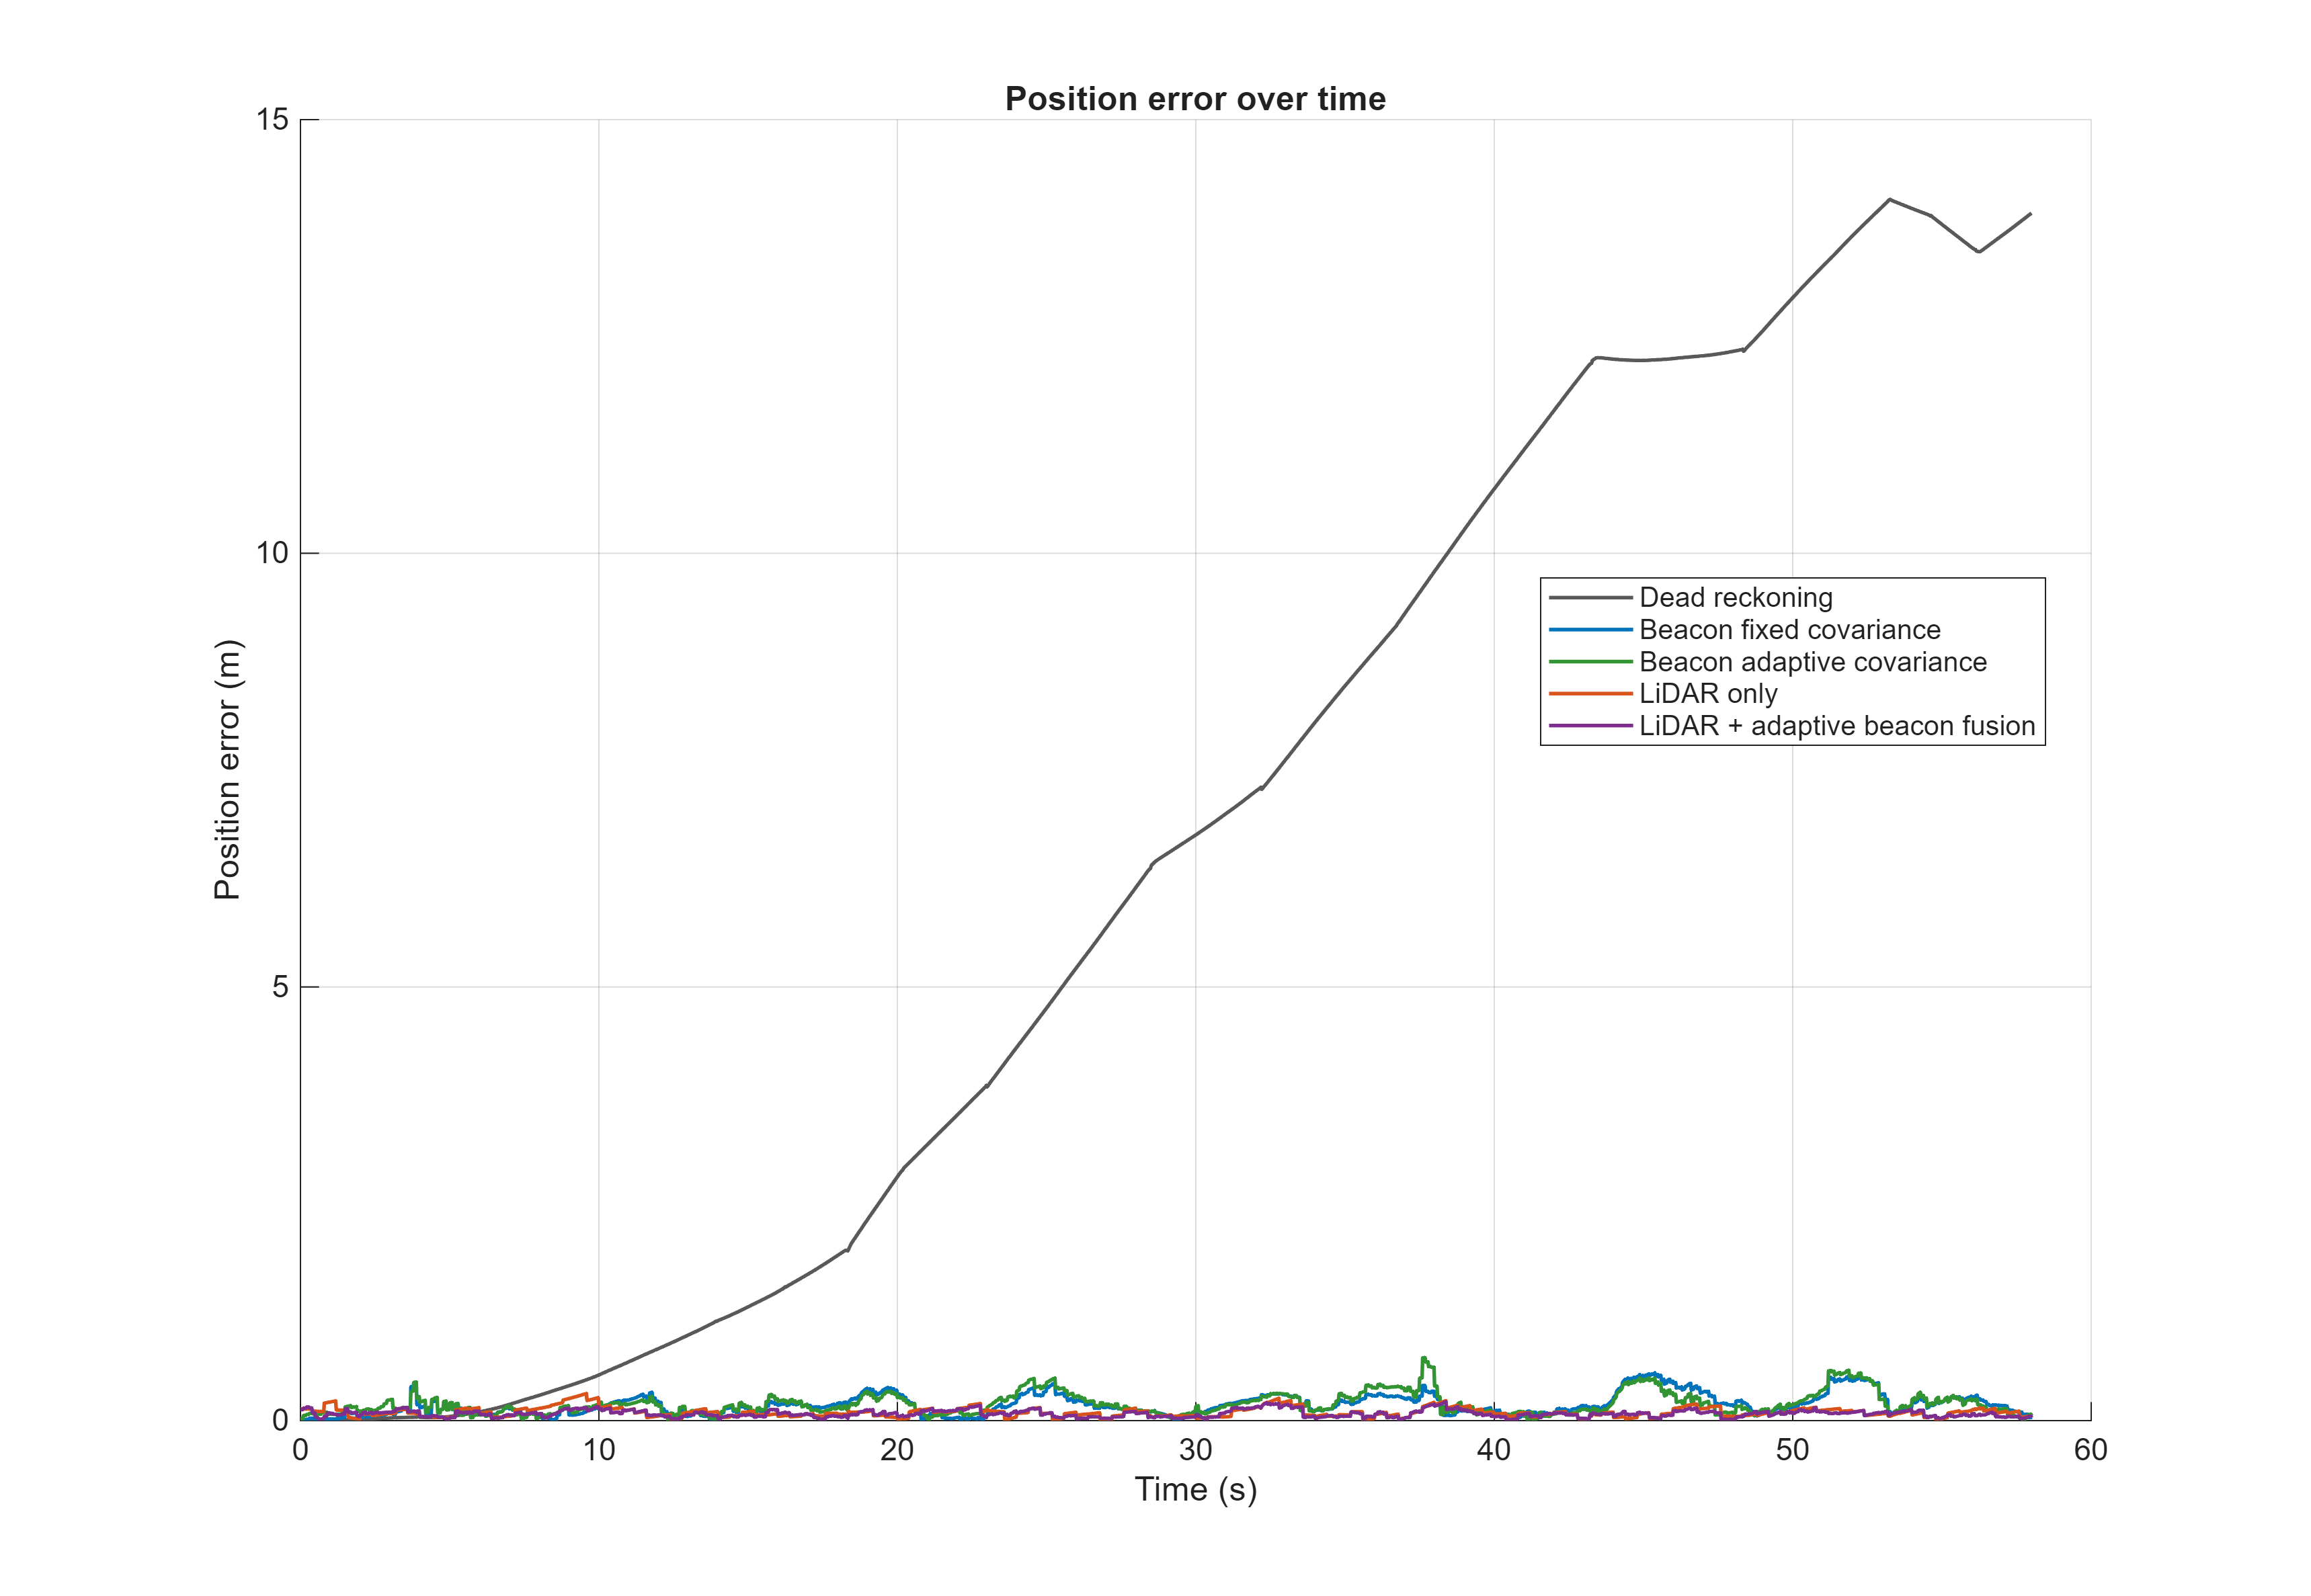
\includegraphics[width=0.30\textwidth]{scenario_001_fig_position_error.png} &
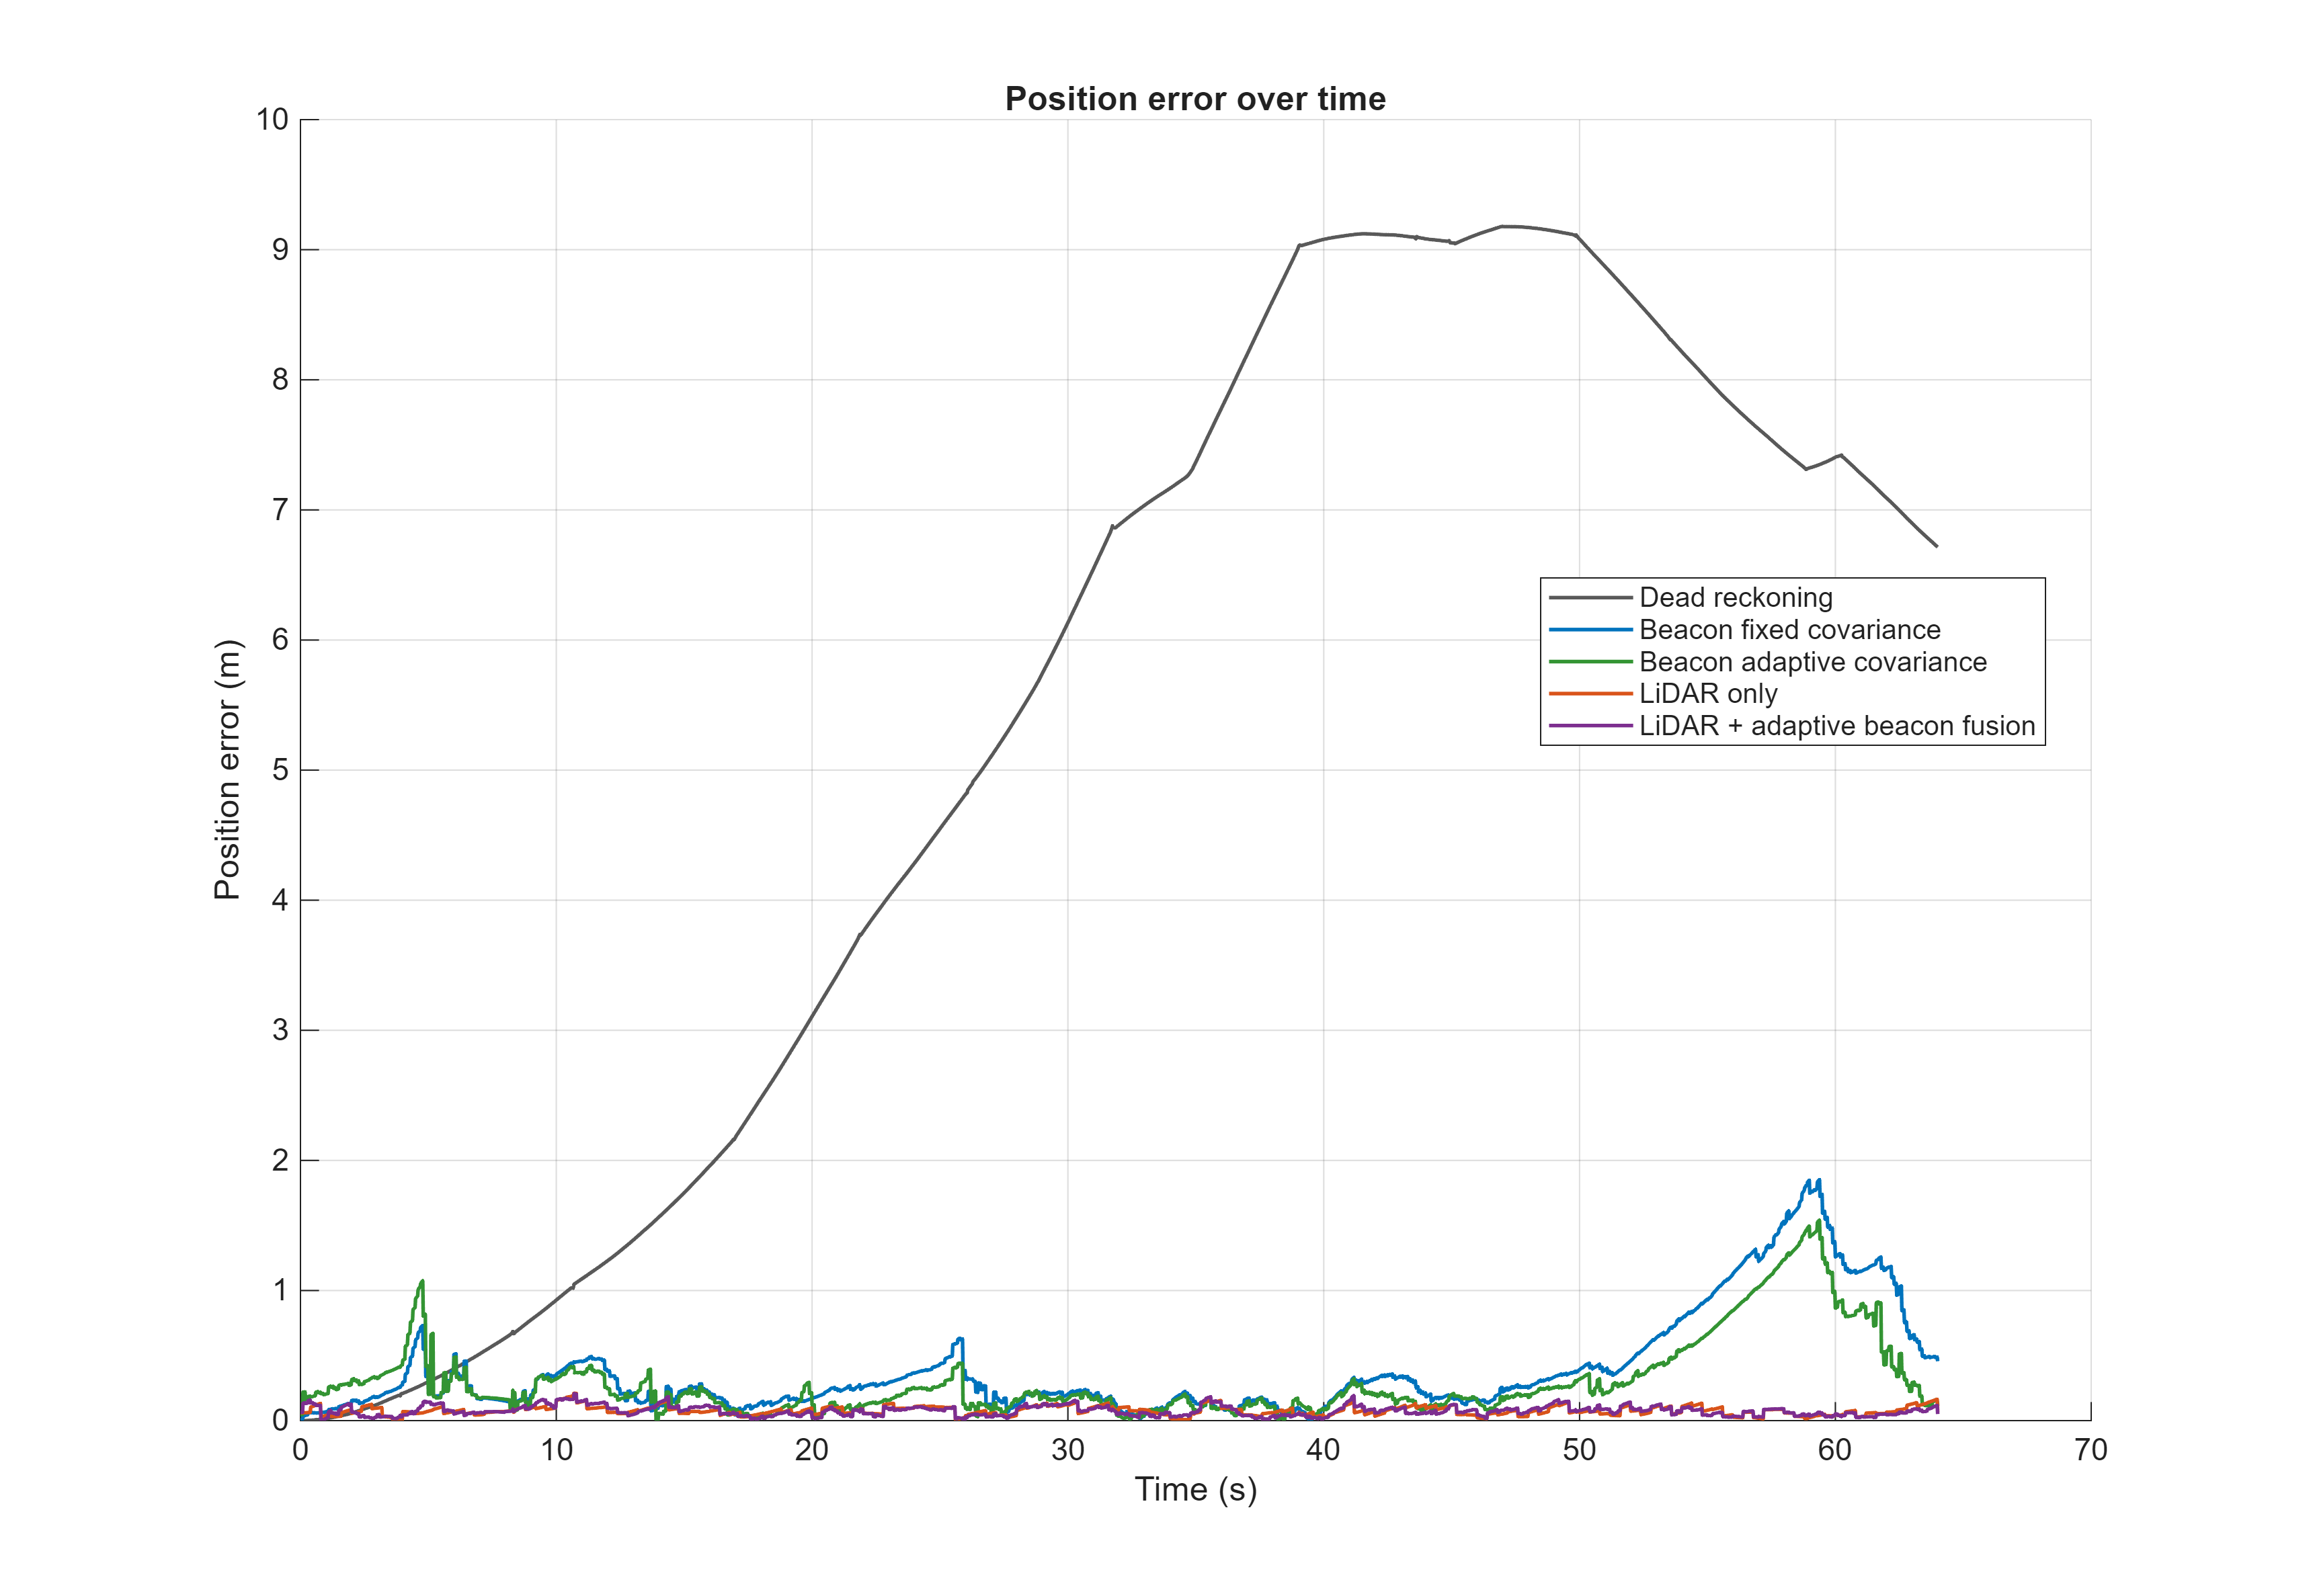
\includegraphics[width=0.30\textwidth]{scenario_002_fig_position_error.png} &
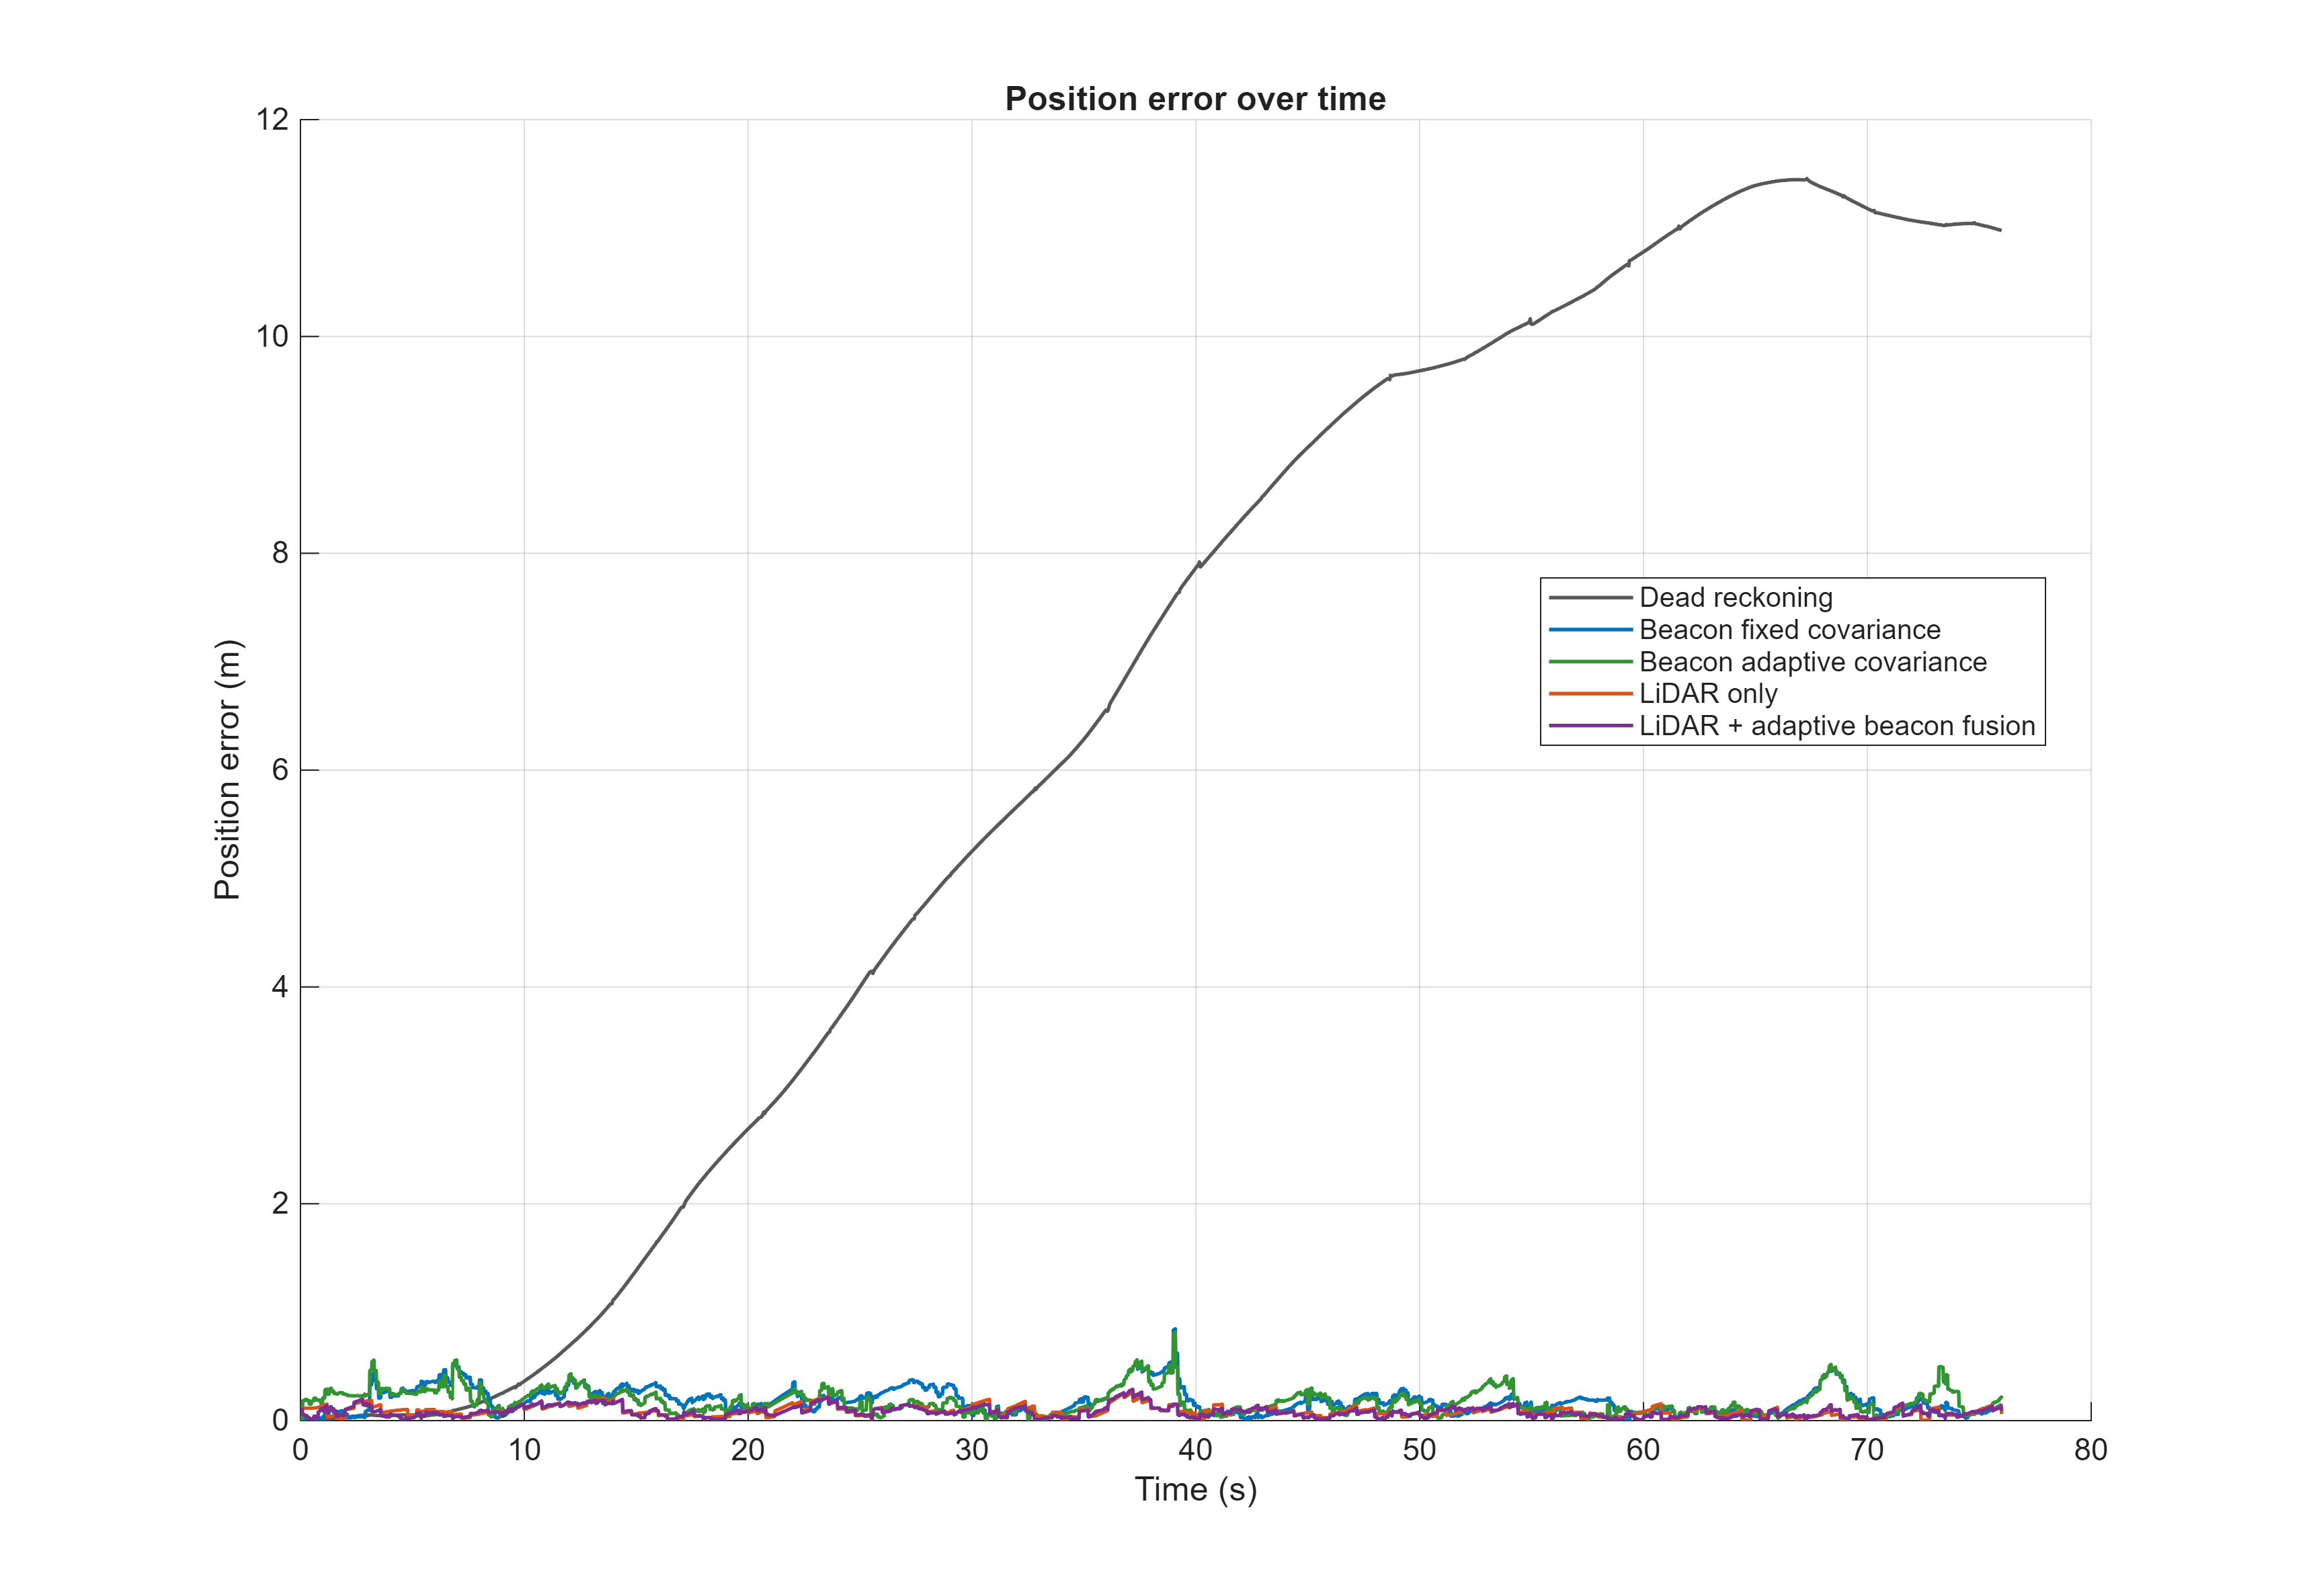
\includegraphics[width=0.30\textwidth]{scenario_003_fig_position_error.png}\\
(a) Scenario 1 & (b) Scenario 2 & (c) Scenario 3
\end{tabular}
\caption{Position error histories for all three scenarios.}
\label{fig:position_errors}
\end{figure*}

\begin{figure*}
\centering
\begin{tabular}{ccc}
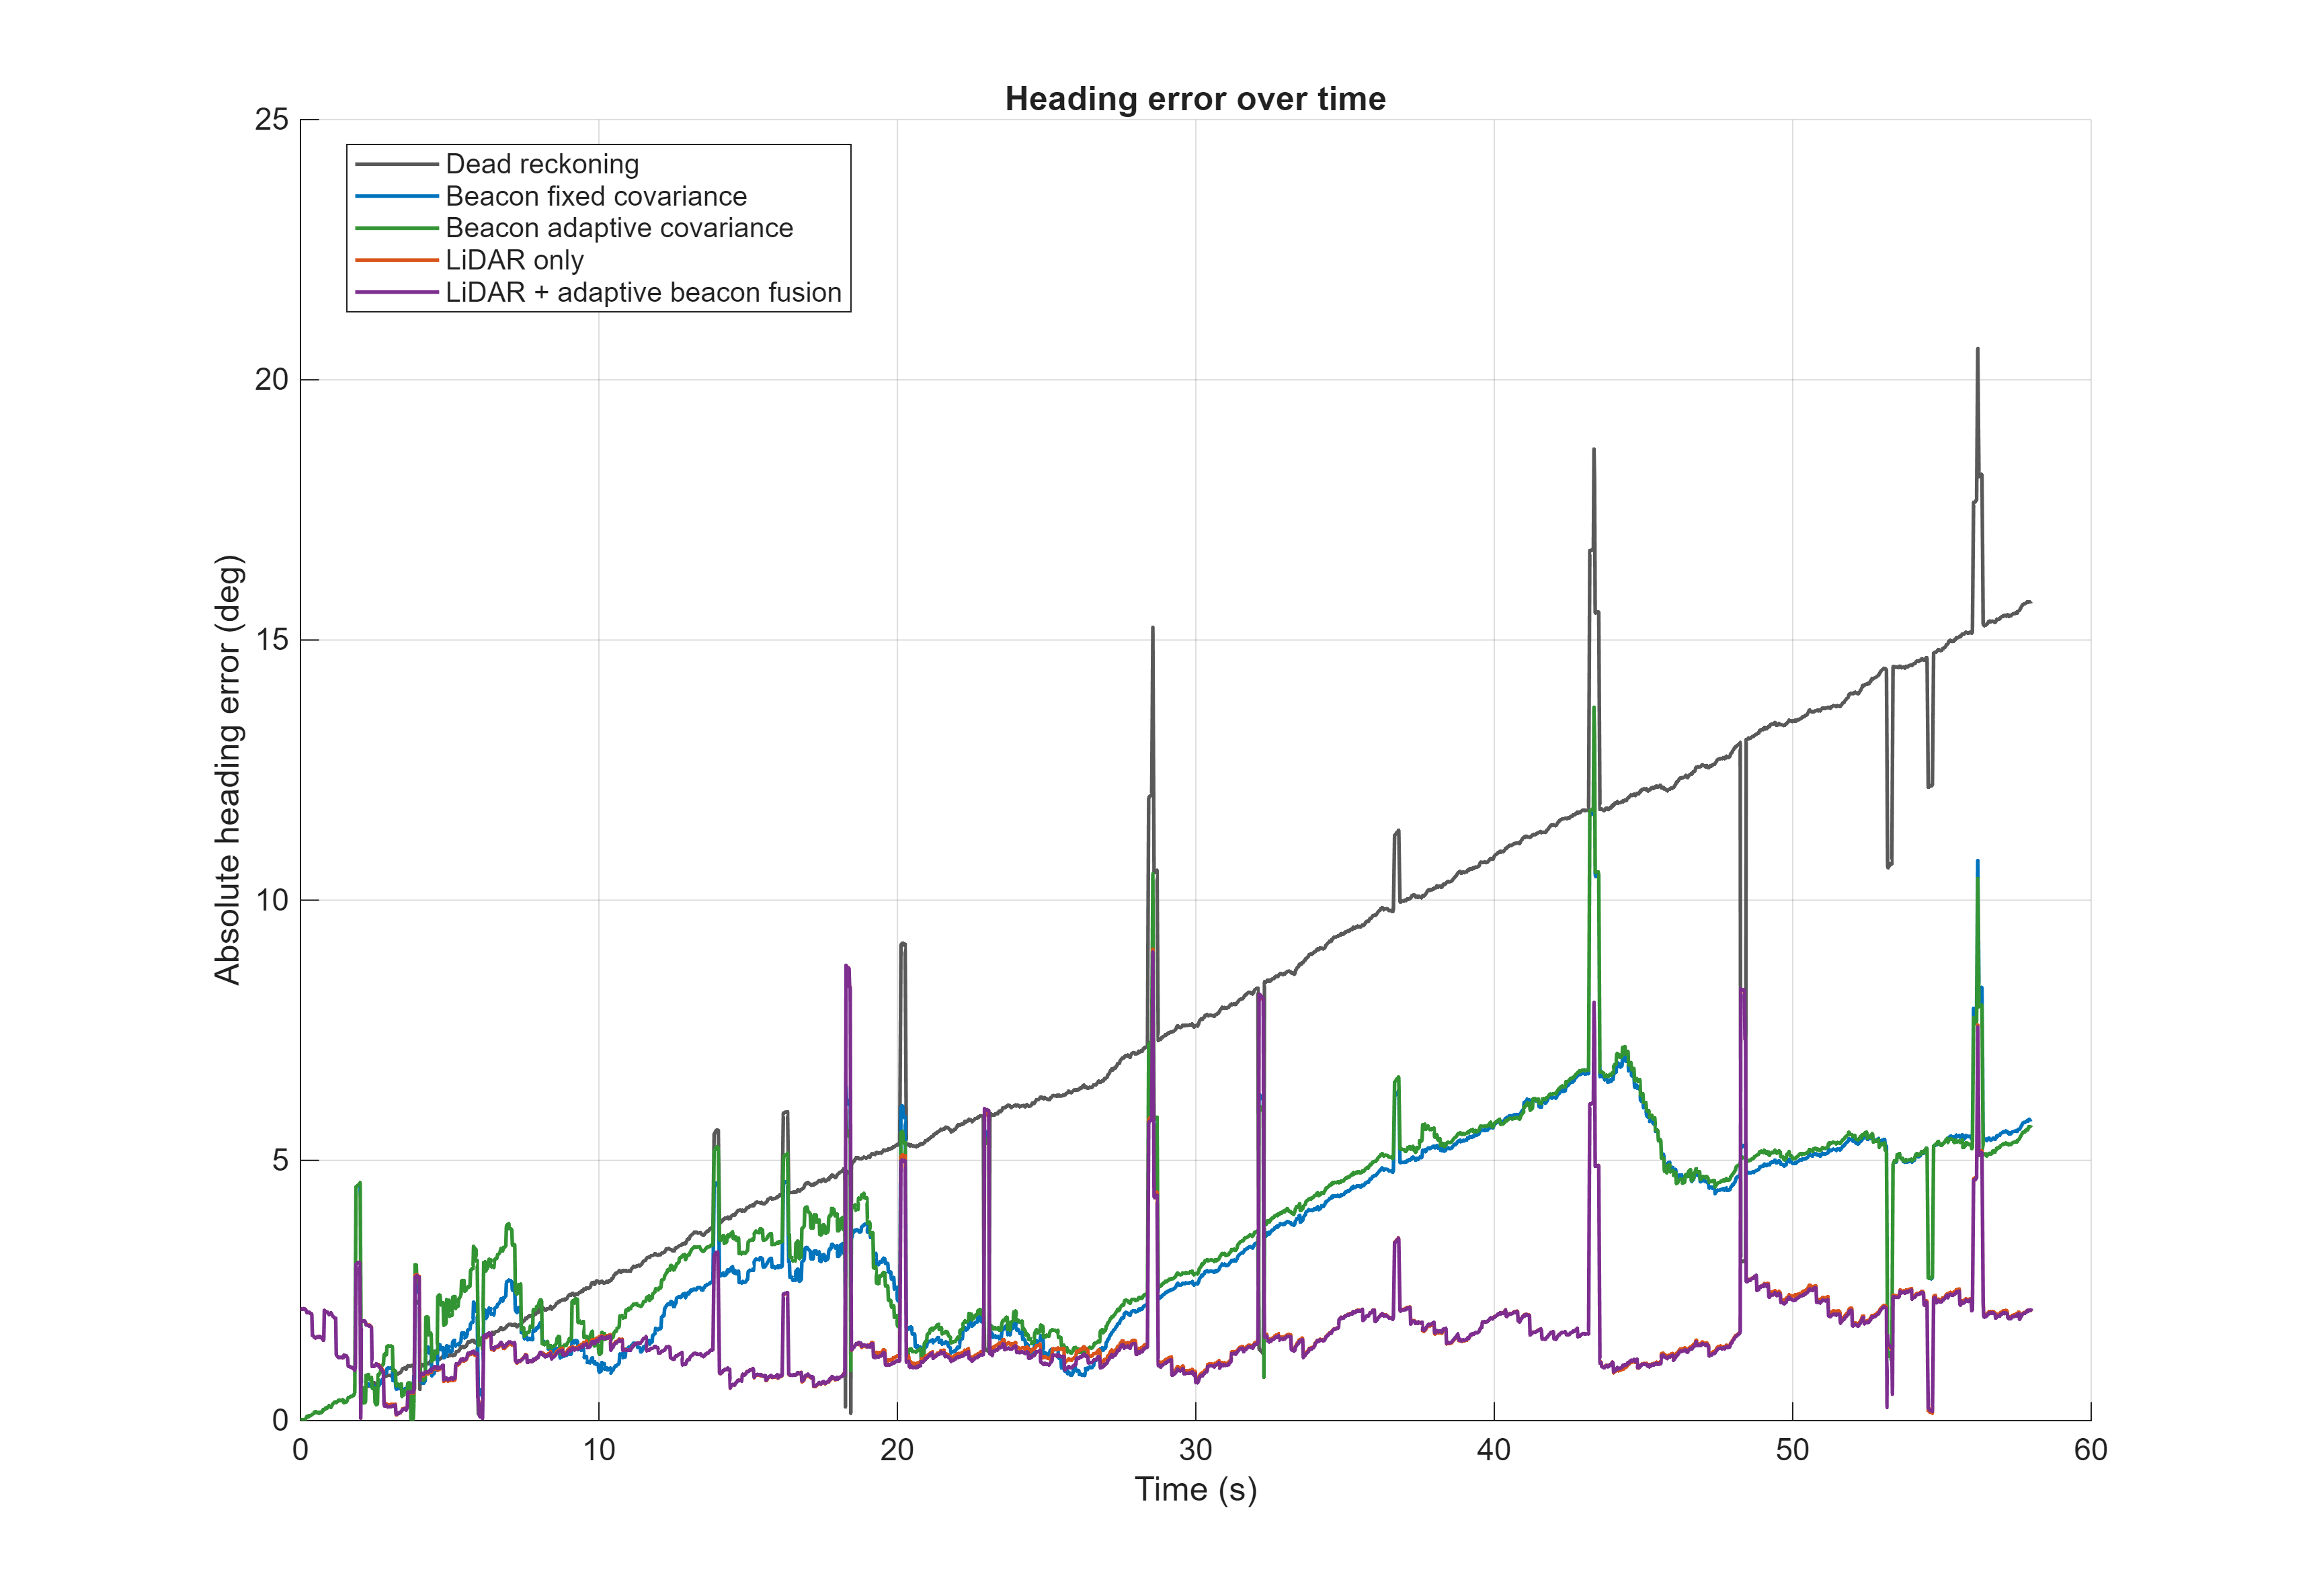
\includegraphics[width=0.30\textwidth]{scenario_001_fig_heading_error.png} &
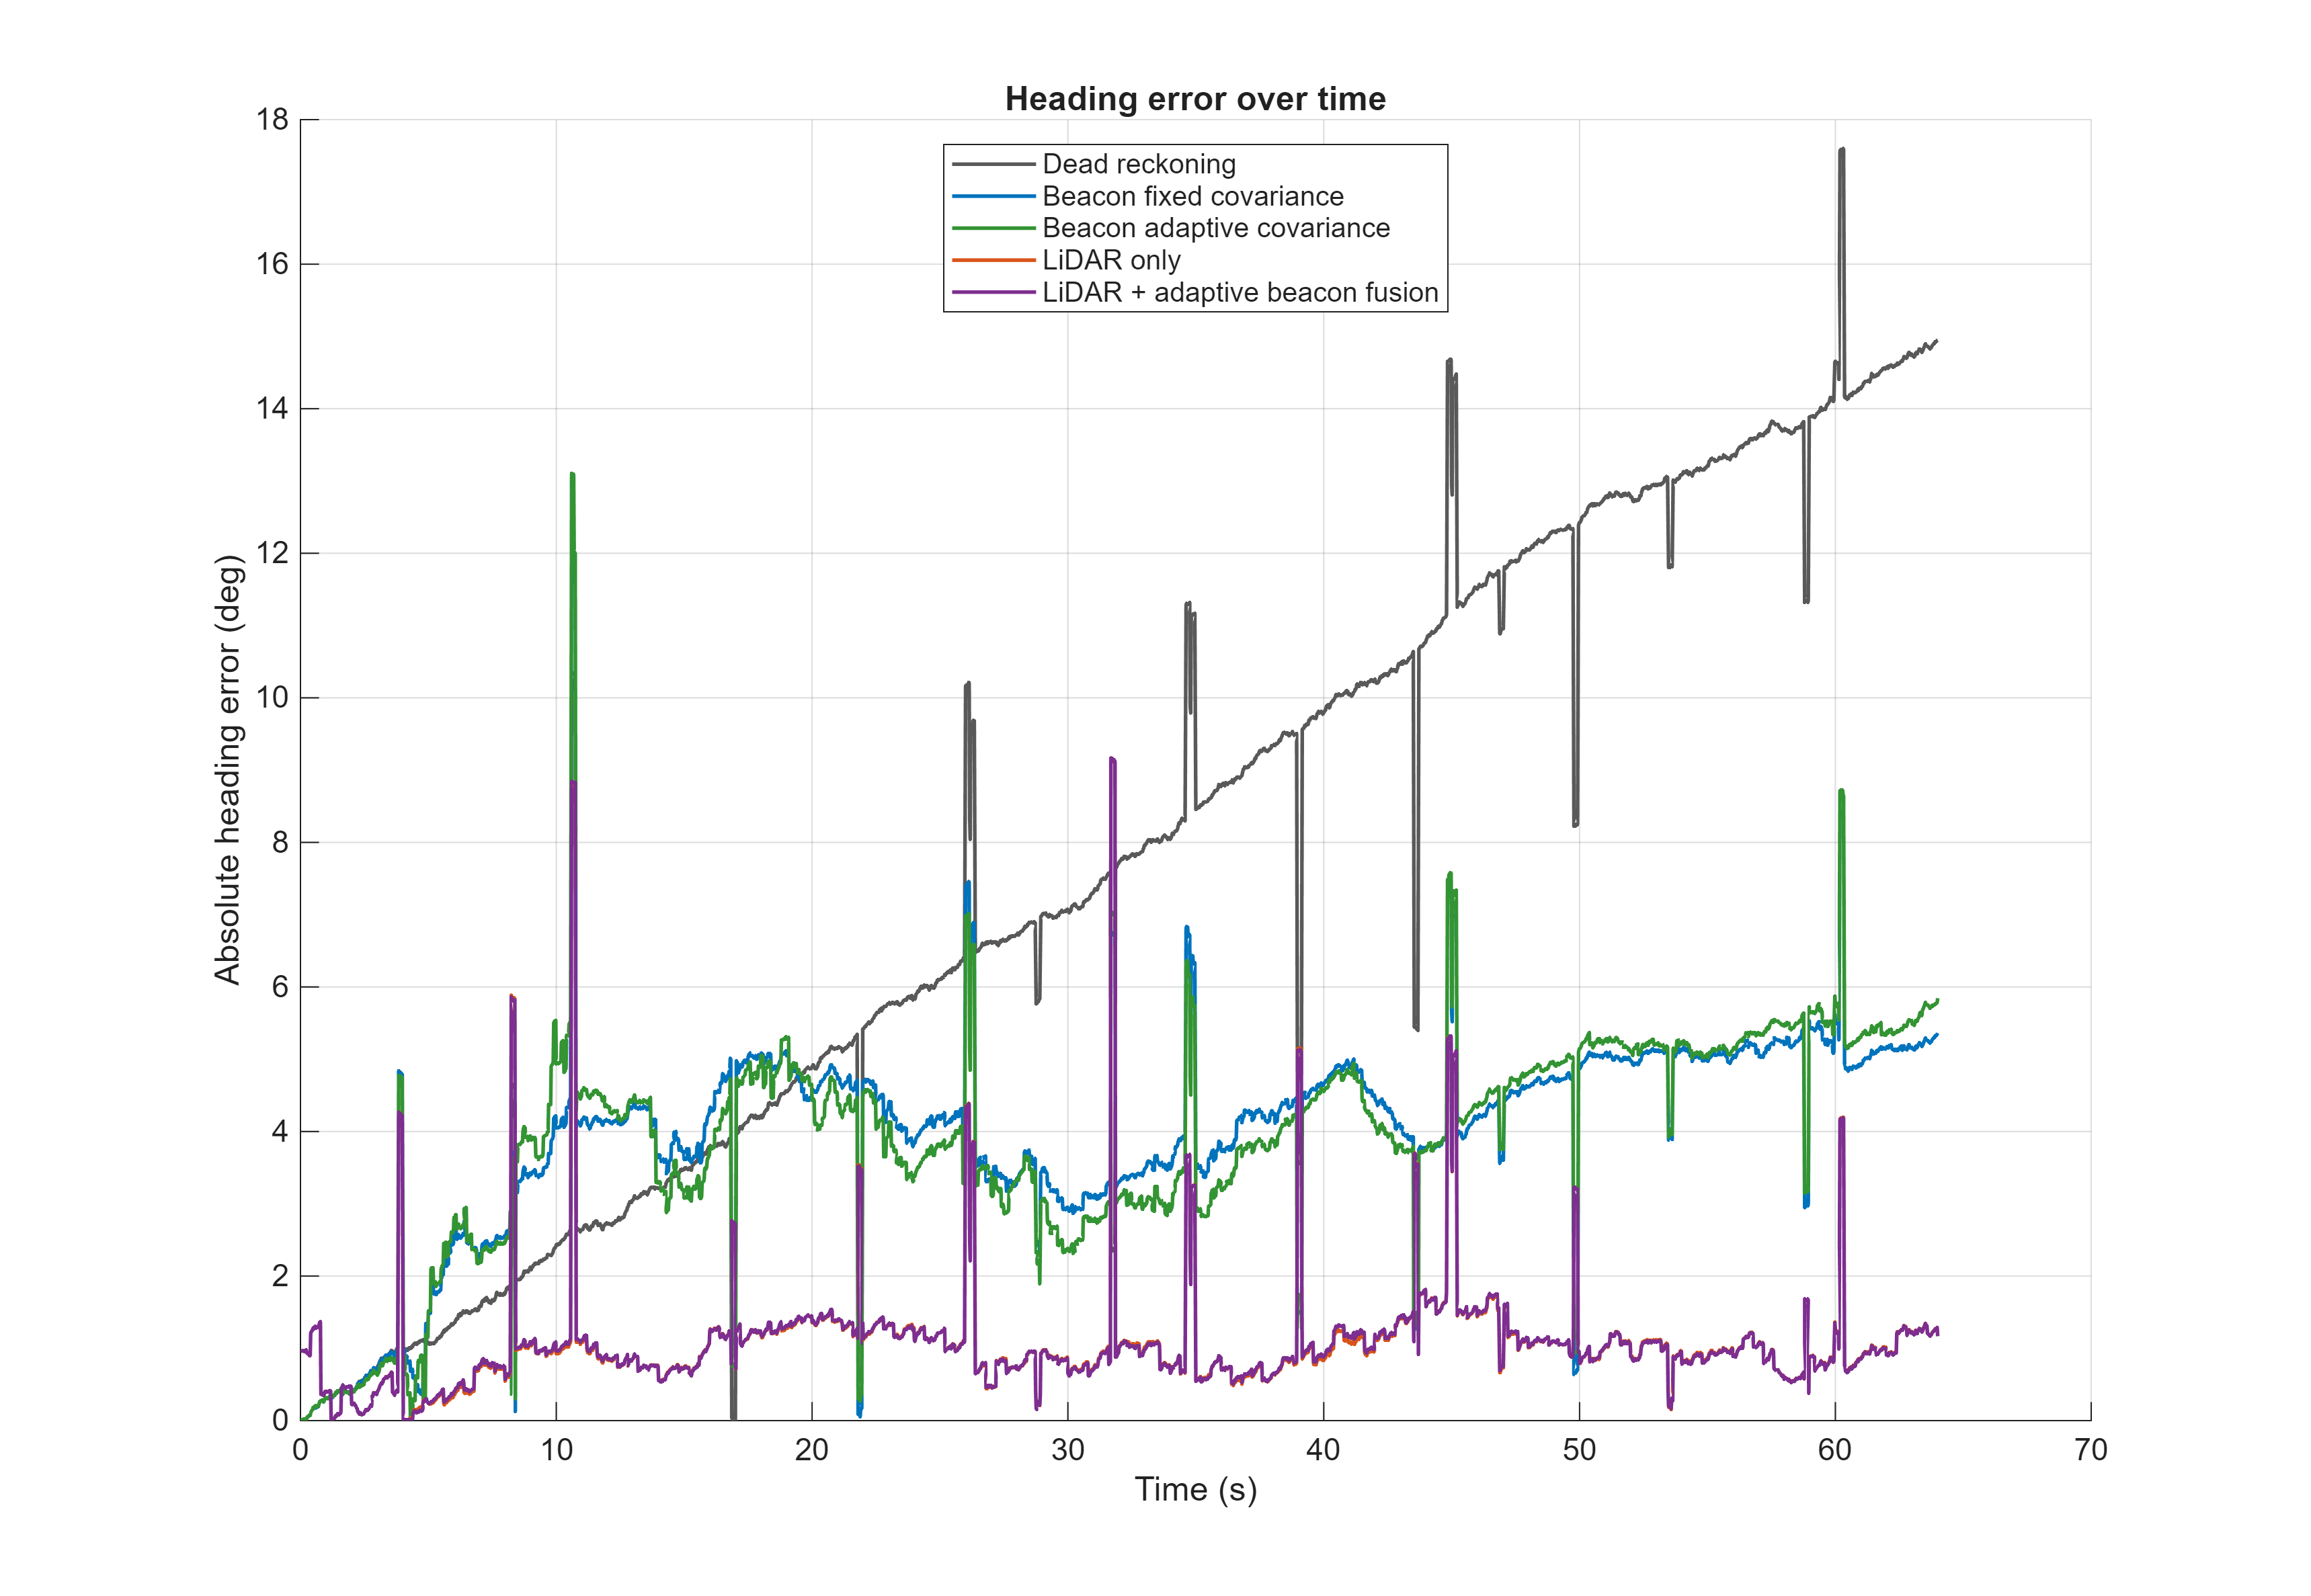
\includegraphics[width=0.30\textwidth]{scenario_002_fig_heading_error.png} &
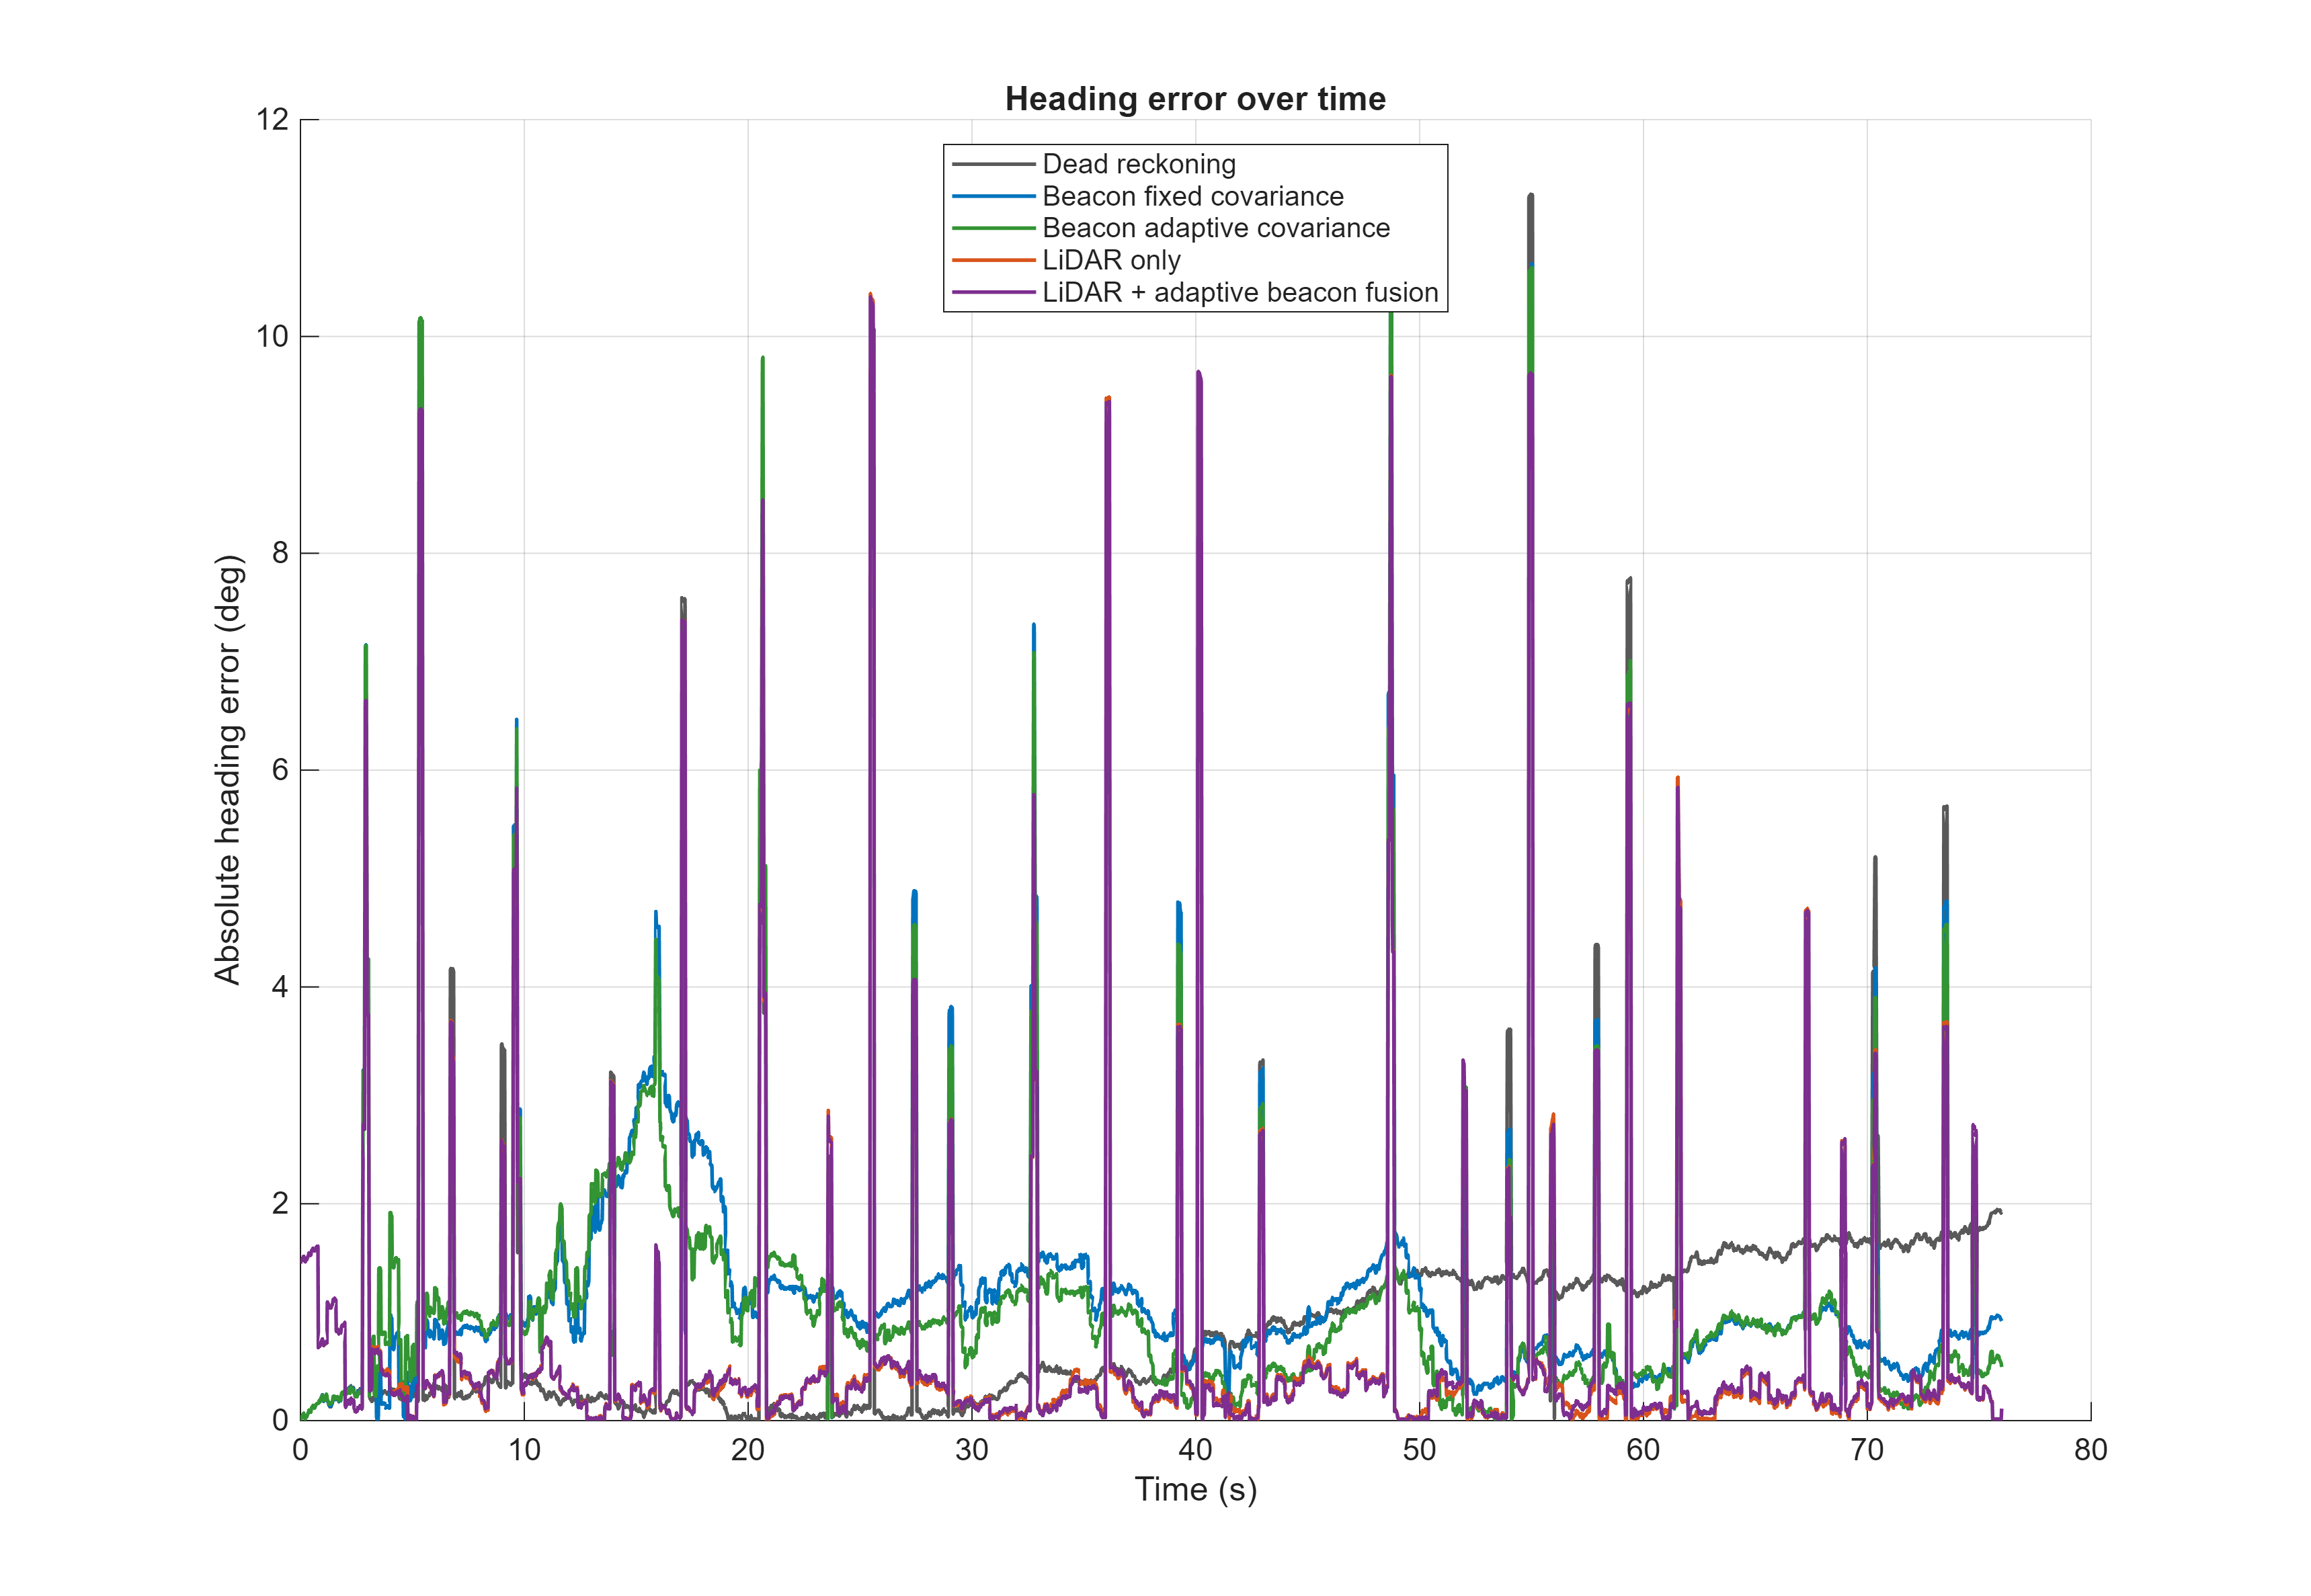
\includegraphics[width=0.30\textwidth]{scenario_003_fig_heading_error.png}\\
(a) Scenario 1 & (b) Scenario 2 & (c) Scenario 3
\end{tabular}
\caption{Heading error histories for all three scenarios.}
\label{fig:heading_errors}
\end{figure*}

\begin{figure*}
\centering
\begin{tabular}{ccc}
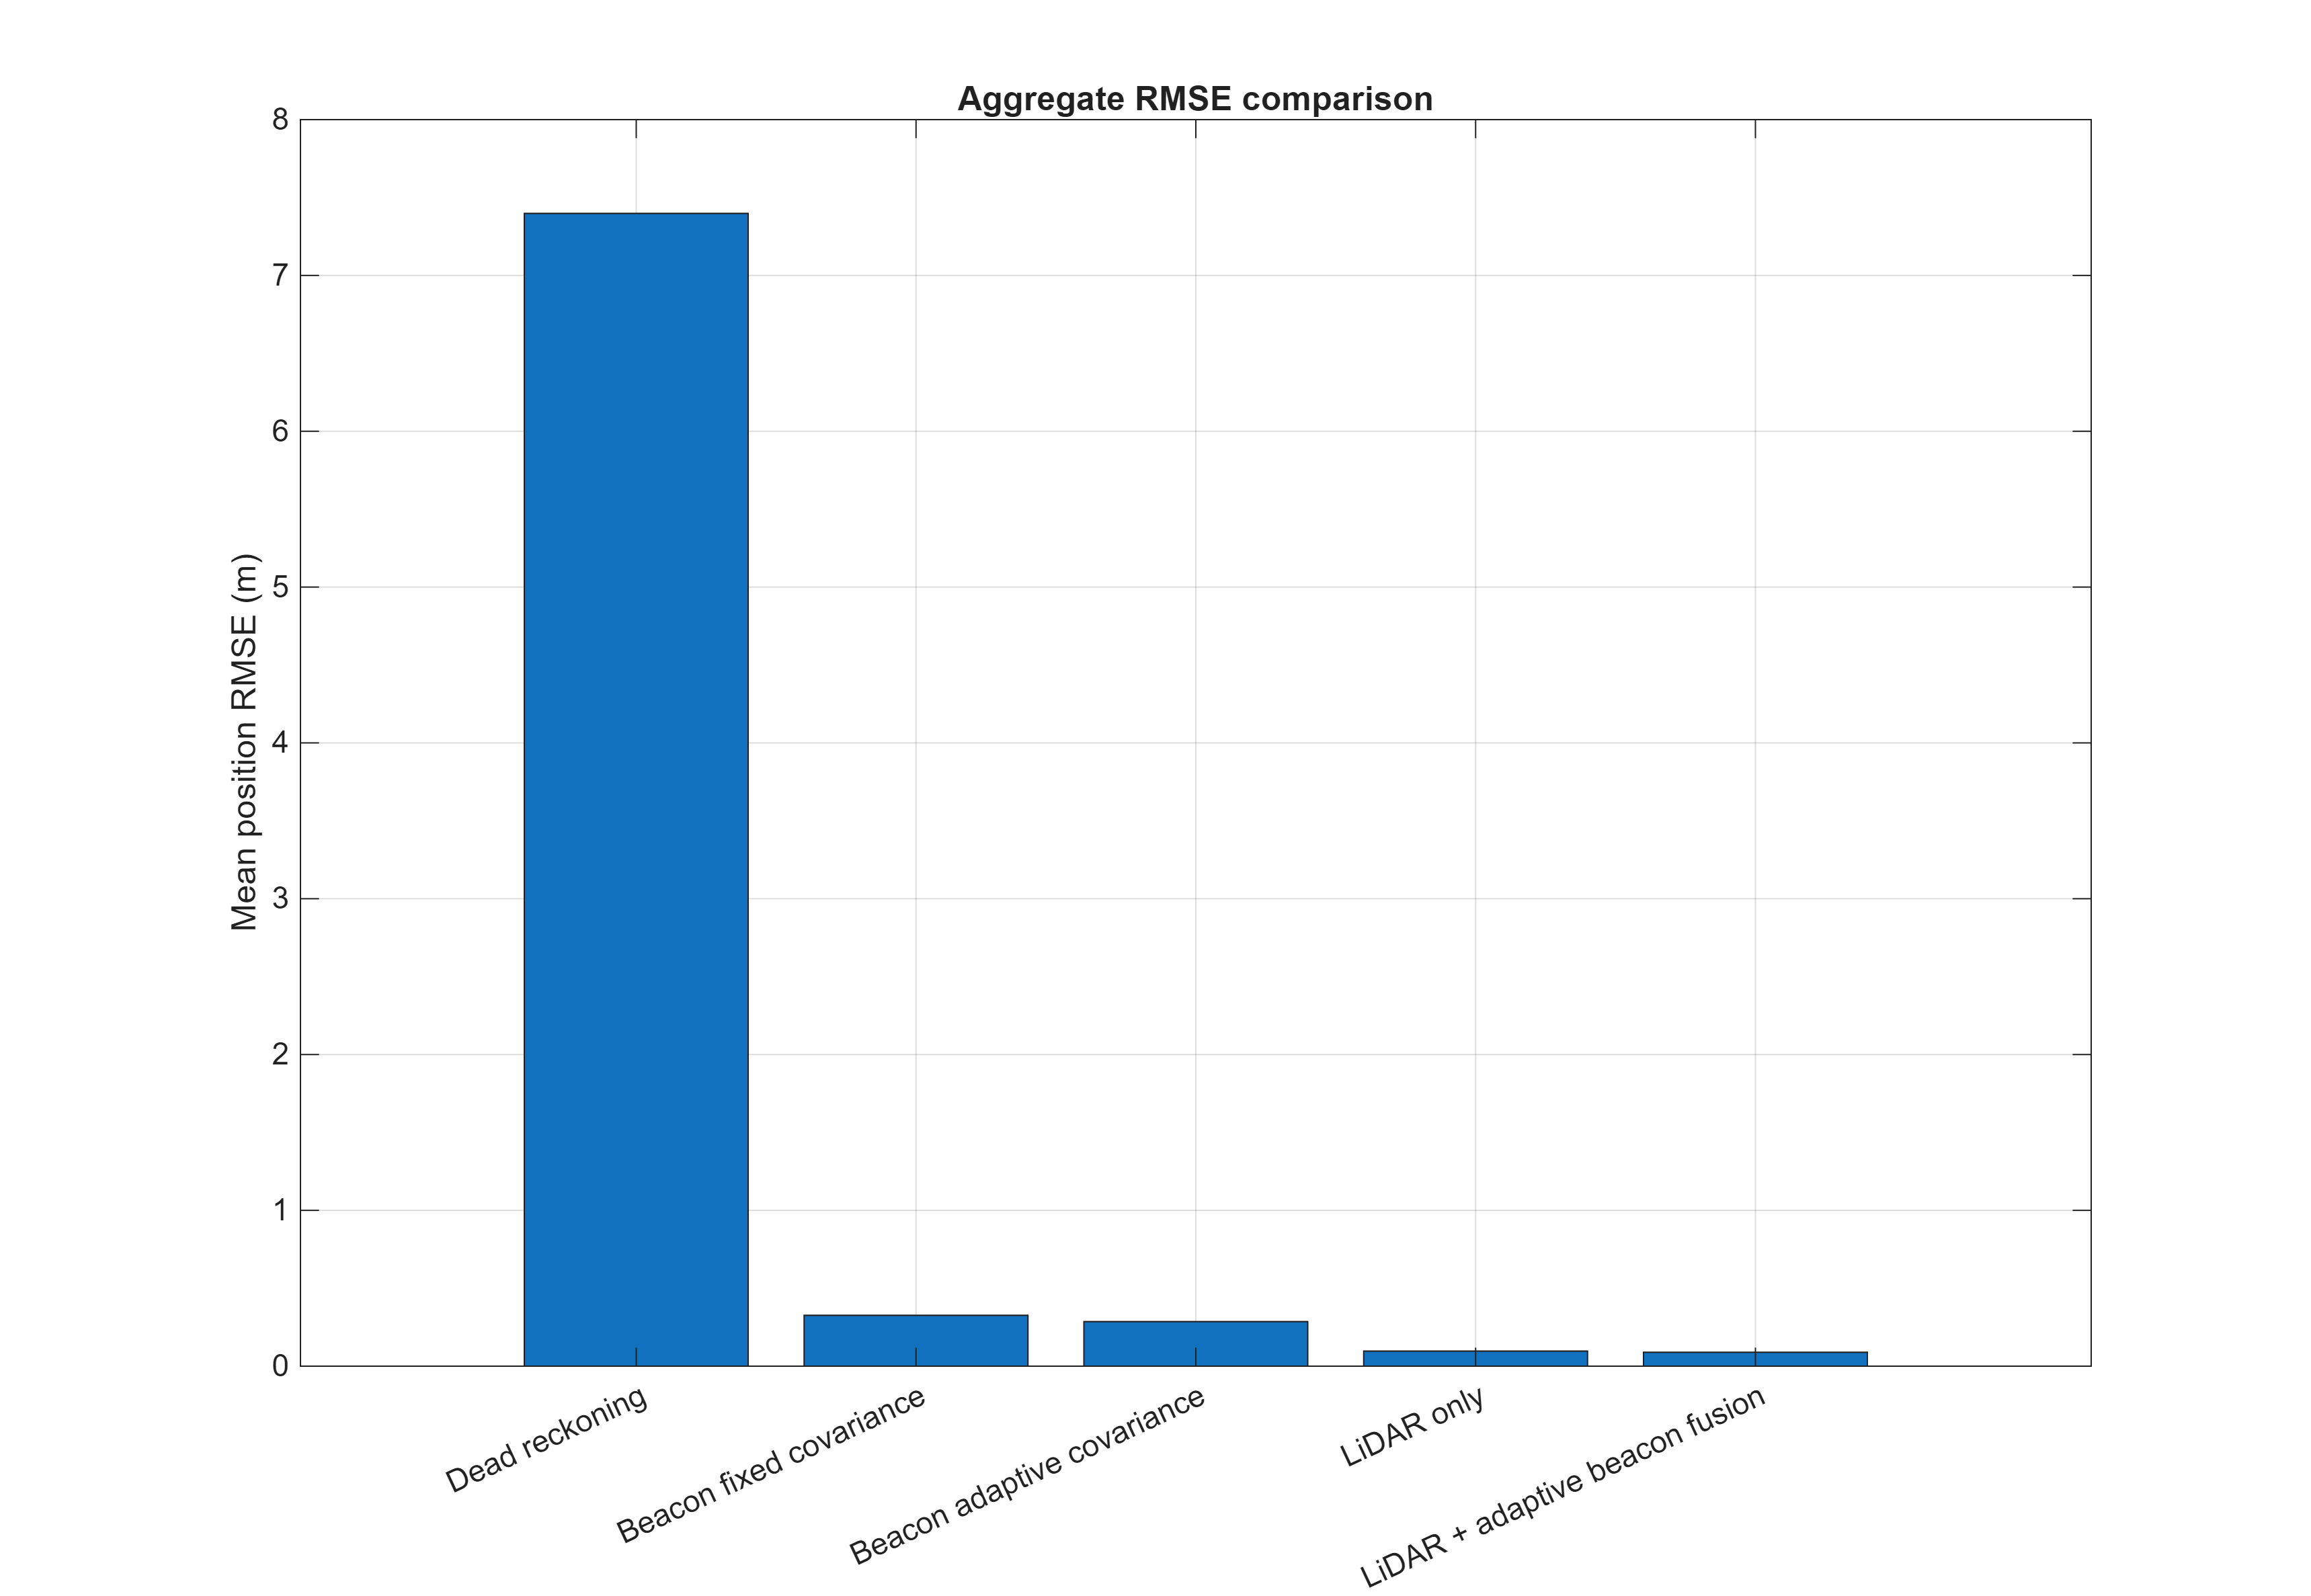
\includegraphics[width=0.30\textwidth]{scenario_001_fig_rmse_comparison.png} &
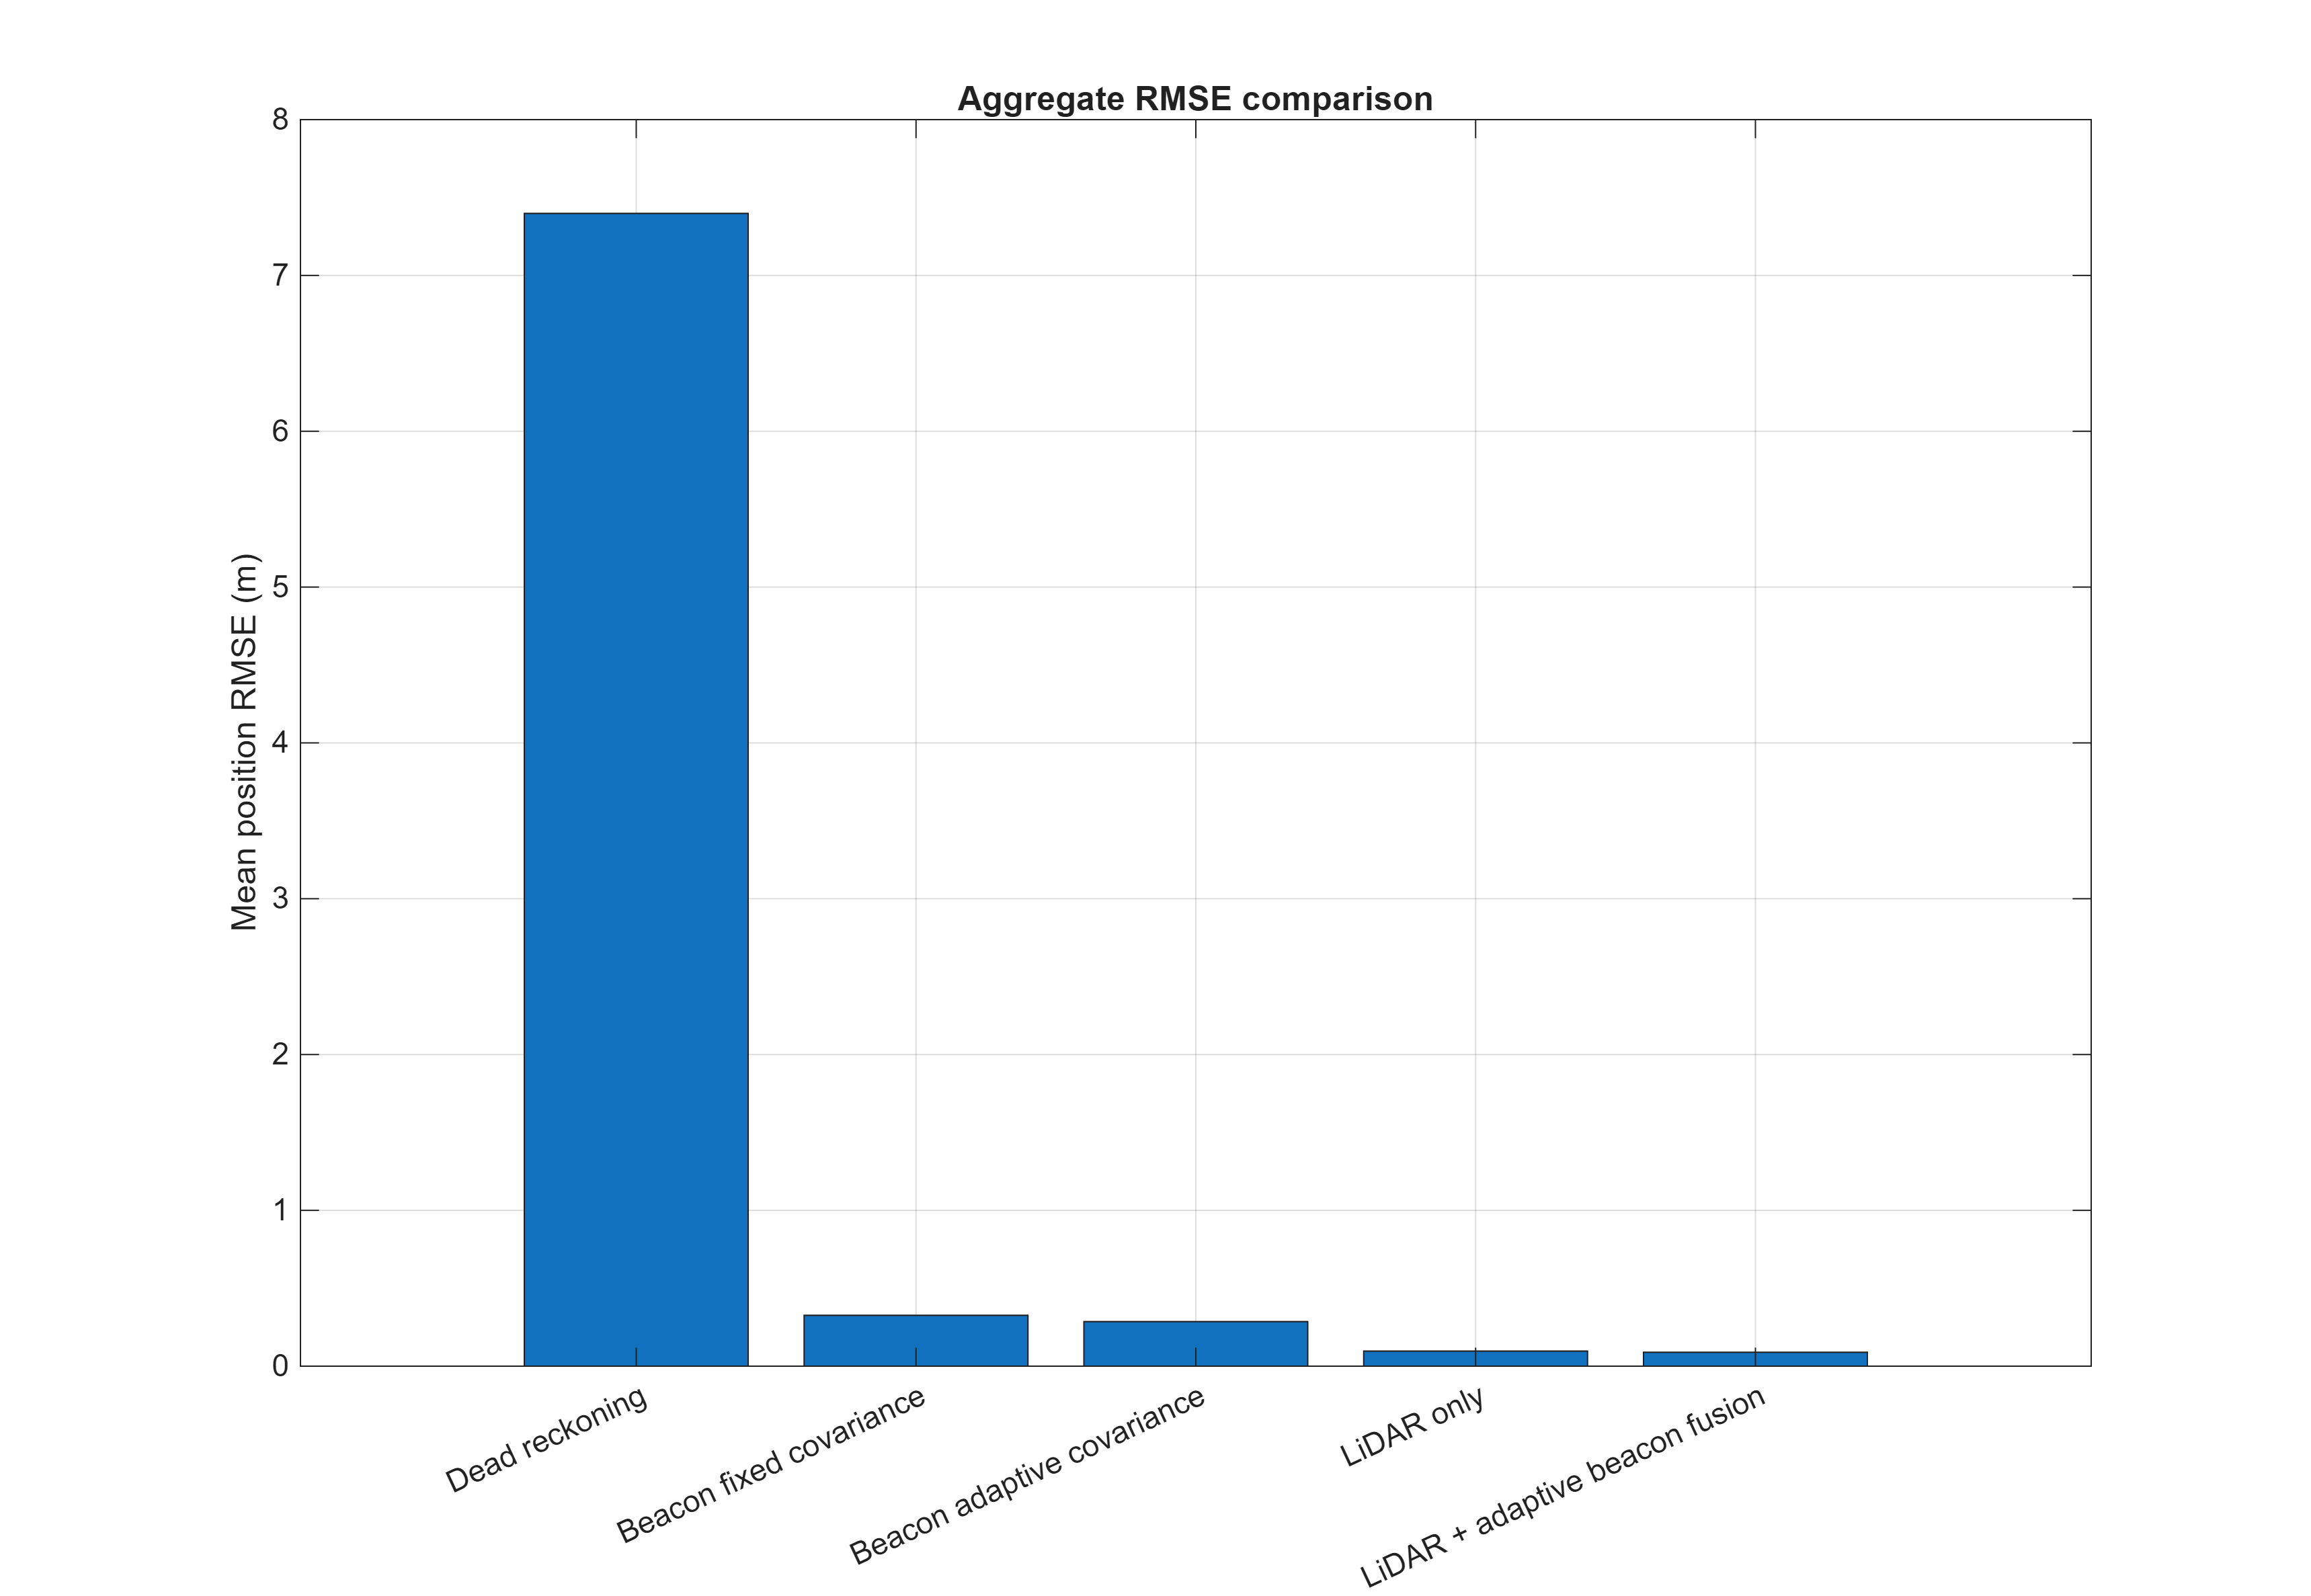
\includegraphics[width=0.30\textwidth]{scenario_002_fig_rmse_comparison.png} &
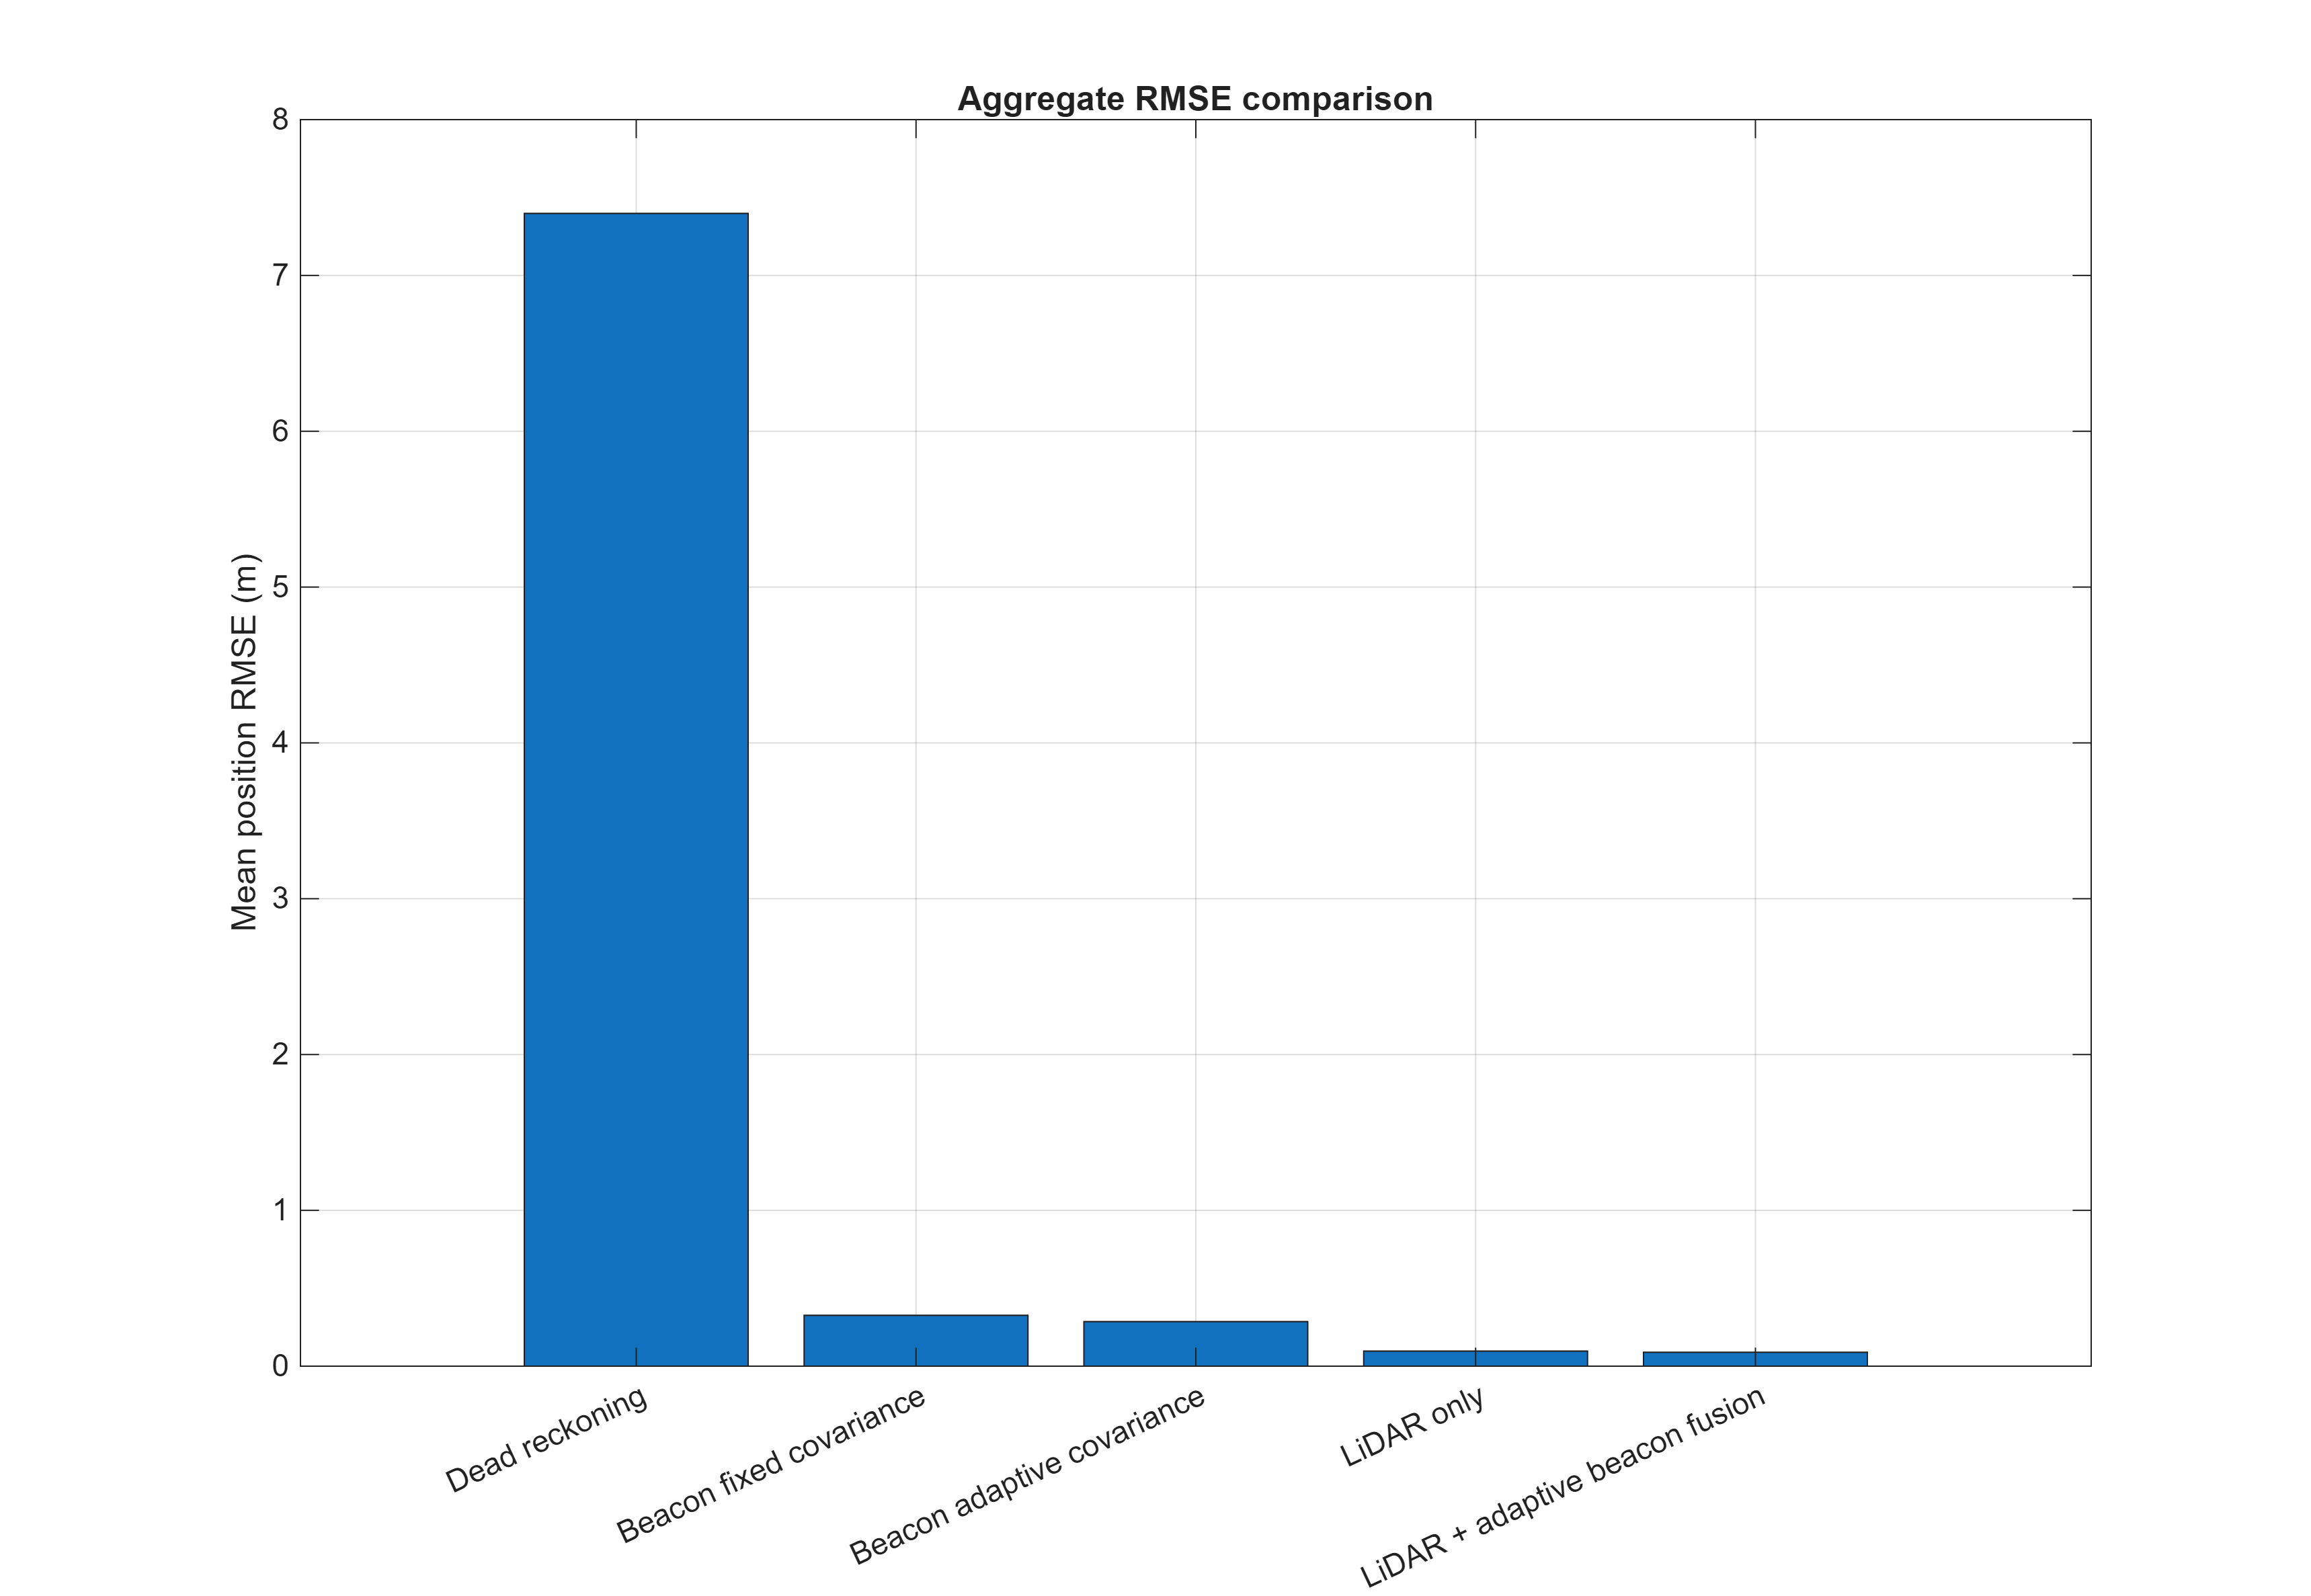
\includegraphics[width=0.30\textwidth]{scenario_003_fig_rmse_comparison.png}\\
(a) Scenario 1 & (b) Scenario 2 & (c) Scenario 3
\end{tabular}
\caption{Scenario-level RMSE comparisons.}
\label{fig:rmse_comparison}
\end{figure*}

\begin{table*}
\centering
\caption{Scenario-level RMSE values.}
\label{tab:rmse}
\begin{tabular}{llrrr}
\toprule
Scenario & Case & Position RMSE (m) & Heading RMSE (rad) & Velocity RMSE (m/s)\\
\midrule
1 & Dead reckoning & 8.270 & 0.157 & 0.367\\
1 & Beacon fixed covariance & 0.219 & 0.070 & 0.142\\
1 & Beacon adaptive covariance & 0.230 & 0.073 & 0.141\\
1 & LiDAR only & 0.109 & 0.034 & 0.087\\
1 & LiDAR + adaptive beacon fusion & 0.089 & 0.034 & 0.085\\
2 & Dead reckoning & 6.286 & 0.156 & 0.285\\
2 & Beacon fixed covariance & 0.544 & 0.074 & 0.133\\
2 & Beacon adaptive covariance & 0.421 & 0.074 & 0.119\\
2 & LiDAR only & 0.083 & 0.025 & 0.065\\
2 & LiDAR + adaptive beacon fusion & 0.083 & 0.025 & 0.065\\
3 & Dead reckoning & 7.638 & 0.031 & 0.222\\
3 & Beacon fixed covariance & 0.215 & 0.033 & 0.141\\
3 & Beacon adaptive covariance & 0.207 & 0.032 & 0.136\\
3 & LiDAR only & 0.099 & 0.026 & 0.117\\
3 & LiDAR + adaptive beacon fusion & 0.095 & 0.026 & 0.117\\
\bottomrule
\end{tabular}
\end{table*}

\begin{table}
\centering
\caption{Aggregate RMSE values across the three scenarios.}
\label{tab:aggregate}
\begin{tabular}{lrrr}
\toprule
Case & Pos. (m) & Head. (rad) & Vel. (m/s)\\
\midrule
Dead reckoning & 7.398 & 0.115 & 0.291\\
Beacon fixed & 0.326 & 0.059 & 0.139\\
Beacon adaptive & 0.286 & 0.059 & 0.132\\
LiDAR only & 0.0968 & 0.0285 & 0.0895\\
LiDAR + beacon & 0.0891 & 0.0284 & 0.0890\\
\bottomrule
\end{tabular}
\end{table}

\begin{table}
\centering
\scriptsize
\caption{Sensor availability.}
\label{tab:availability}
\begin{tabular}{lrrr}
\toprule
Scenario & Beacon (\%) & Mean beacons & LiDAR (\%)\\
\midrule
1 & 28.7 & 1.72 & 95.9\\
2 & 21.4 & 1.49 & 99.4\\
3 & 16.4 & 1.48 & 94.8\\
\bottomrule
\end{tabular}
\end{table}

Obtained results show the expected drift of the prediction-only baseline. Dead reckoning produces position RMSE values from 6.286 m to 8.270 m, with a three-scenario mean of 7.398 m. Beacon updates reduce the aggregate position RMSE by more than an order of magnitude relative to dead reckoning. The adaptive beacon covariance improves the aggregate beacon-only position RMSE from 0.326 m to 0.286 m and the aggregate velocity RMSE from 0.139 m/s to 0.132 m/s. The adaptive model is not uniformly better in every individual case: in Scenario 1, fixed beacon covariance gives 0.219 m position RMSE while adaptive covariance gives 0.230 m.

The LiDAR pose update is the strongest individual correction source in these generated experiments. LiDAR-only filtering gives a mean position RMSE of 0.0968 m. Adding adaptive beacon updates gives a mean position RMSE of 0.0891 m. The fused case improves over LiDAR-only in Scenarios 1 and 3, while Scenario 2 is essentially unchanged at the displayed precision. Heading RMSE follows the same pattern: the LiDAR-only and fused cases have aggregate heading RMSE values near 0.028 rad, lower than the beacon-only cases.

Sensor availability decreases with scenario complexity for beacons. The per-beacon measurement availability is 28.7\% in Scenario 1, 21.4\% in Scenario 2, and 16.4\% in Scenario 3. Average available beacons per beacon update remain between 1.48 and 1.72, so many beacon updates are geometrically limited. LiDAR pose availability remains high, between 94.8\% and 99.4\%, because the generated maps usually provide enough valid ray-cast returns and scan quality for the synthetic pose measurement.

\section{Discussion}

The results support the main implementation hypothesis only in the aggregate and with important qualifications. Adaptive beacon covariance improves beacon-only mean position RMSE relative to fixed covariance, and it improves the beacon-only velocity RMSE in all three scenarios. However, the adaptive beacon filter is slightly worse than the fixed-covariance beacon filter in Scenario 1 position RMSE. The evidence therefore favors adaptive covariance as a useful model for these saved data, not as a uniformly dominant choice for every trajectory and beacon geometry.

The fused LiDAR plus adaptive beacon case gives the lowest aggregate position RMSE, but the margin over LiDAR-only filtering is modest because the synthetic LiDAR pose measurements are frequent and usually available. This behavior is consistent with the availability table: beacon measurements are intermittent and often underdetermined, while LiDAR pose availability remains above 94\% in all scenarios.

The implementation has several limitations that affect interpretation. First, the filter initializes from the first truth state, so the experiments evaluate propagation and measurement-update behavior rather than global initialization. Second, the LiDAR backend uses synthetic pose measurements generated from truth and scan quality; raw scan matching is not implemented. Third, the RSSI model is a linear synthetic attenuation model, and the filter only adapts covariance from measured range and RSSI. Fourth, acceleration and gyro biases are injected into prediction inputs but are not included in the filter state. These choices are consistent with the repository scope, but they limit claims about real hardware performance.

\section{Conclusion}

The experiments show that adaptive beacon weighting is useful in this simulation setup, but the final fused accuracy is still mainly driven by the LiDAR pose updates. The main takeaways are summarized below.

\begin{enumerate}
    \item \textbf{Adaptive beacon covariance helps in the beacon-only setting.}
    \begin{itemize}
        \item Adaptive beacon covariance improves the aggregate beacon-only position RMSE from 0.326 m to 0.286 m.

        \item It also improves beacon-only velocity RMSE across all three scenarios.

        \item This suggests that beacon measurements should be weighted based on measurement quality instead of using one fixed covariance value for all updates.
    \end{itemize}

    \item \textbf{The improvement is useful, but not universal.}
    \begin{itemize}
        \item The adaptive beacon filter is not better in every individual case.

        \item In Scenario 1, the fixed-covariance beacon filter gives slightly better position RMSE.

        \item Therefore, the result supports adaptive covariance as a useful design choice for these experiments, not as a guaranteed improvement for every map, trajectory, or beacon layout.
    \end{itemize}

    \item \textbf{LiDAR is the main driver of fused localization accuracy.}
    \begin{itemize}
        \item The fused LiDAR plus adaptive beacon filter gives the best aggregate position RMSE at 0.0891 m.

        \item The improvement over the LiDAR-only filter is modest because the LiDAR pose measurements are frequent and usually available.

        \item Since beacon measurements are intermittent and sometimes underdetermined, they mainly act as supporting corrections rather than the dominant source of localization accuracy.
    \end{itemize}

    \item \textbf{Limitations of the study.}
    \begin{itemize}
        \item The filter starts from the first truth state, so the study does not test global initialization.

        \item The LiDAR backend uses synthetic pose measurements instead of raw scan matching.

        \item The RSSI and attenuation models are synthetic, and sensor biases are not estimated as part of the filter state.

        \item These assumptions keep the experiment reproducible, but they limit direct claims about real hardware performance.
    \end{itemize}
\end{enumerate}

Overall, the strongest conclusion supported by the data is that adaptive beacon weighting improves beacon-only localization in aggregate, while LiDAR pose corrections dominate the best fused localization results.
\appendix
\section{Implementation-Related Mathematical Background}

\subsection{Manifolds}

A differentiable manifold is a space that is locally vector-like but not necessarily globally Euclidean. Robot orientation is the relevant example in this repository: the heading angle represents an element of \(\SO(2)\), and angles wrap modulo \(2\pi\). Treating orientation as an unconstrained Euclidean coordinate can produce ambiguous differences unless corrections are interpreted in local coordinates.

GTSAM formalizes this distinction through \texttt{retract} and \texttt{localCoordinates}: \texttt{retract} maps a tangent vector at a state back onto the manifold, while \texttt{localCoordinates} computes a tangent vector between two states \citep{gtsamConcepts,gtsamPose2,gtsamPose3}. This implementation uses the same idea. The EKF computes \(\delta x\in\R^5\), converts it to the local group increment \(\delta_{\mathrm{group}}\), and retracts it by
\[
    X^{+}=X\Exp(\delta_{\mathrm{group}}).
\]
Thus the covariance is Euclidean only in the tangent space. The nominal state remains a valid NavState matrix after every prediction and correction.

\subsection{Lie Algebra}

A Lie group is both a smooth manifold and a group. Its Lie algebra is the tangent space at the identity. For a planar pose, the group \(\SE(2)\) combines a rotation and a translation, and the exponential map converts a small tangent vector into a finite rigid-body transform. GTSAM's \texttt{Pose2} and \texttt{Pose3} documentation describes this pattern for \(\SE(2)\) and \(\SE(3)\) \citep{gtsamPose2,gtsamPose3}.

The repository uses a 2D NavState extension with tangent coordinates \(\delta=(\phi,\rho_x,\rho_y,\nu_x,\nu_y)\). A corresponding algebra element can be written schematically as
\[
\delta^\wedge =
\begin{bmatrix}
\phi S_2 & \rho & \nu\\
0_{1\times 2} & 0 & 0\\
0_{1\times 2} & 0 & 0
\end{bmatrix},
\]
where \(S_2\) is the planar skew-symmetric generator. Rather than calling a generic matrix exponential, \texttt{navstate\_exp.m} evaluates the closed-form structure used in Eq.~(\ref{eq:nav_exp}) with a third-order approximation to the left Jacobian. This is the operation used for both prediction increments and EKF correction increments.

Linearization occurs in tangent coordinates. For example, the beacon Jacobian in Eq.~(\ref{eq:beacon_H}) maps a perturbation in \((\delta\theta,\delta p,\delta v)\) to a first-order range residual. After solving the linear Kalman update, the perturbation is pushed back to the manifold by composition. This is the same local-linear, global-nonlinear pattern used by manifold optimization and filtering methods \citep{dellaertKaess2017factor,gtsamConcepts}.

\subsection{Navigation State / NavState}

In GTSAM, \texttt{NavState} represents a navigation state containing attitude, position, and velocity, and the navigation module includes manifold and Lie-group EKF utilities for such states \citep{gtsamNavigation,gtsamNavState}. The implementation here is a planar analog:
\[
    X=(R(\theta),p,v).
\]
It excludes 3D attitude, gravity, IMU bias, and clock terms. The ground robot dynamics are therefore expressed through planar heading, 2D position, and 2D velocity.

The tangent perturbation has five components. The first component perturbs heading; the next two perturb position; the final two perturb velocity. Prediction uses body-frame acceleration and yaw rate to build a local NavState increment. Measurement updates first compute a world-frame EKF correction and then rotate the position and velocity correction into the local frame before calling \(\Exp\). This distinction explains why the filter can use simple Jacobians for world-frame range and pose residuals while still applying the final state update on the NavState manifold.


\bibliographystyle{aasjournalv7}
\bibliography{refs}

\end{document}
